\documentclass[a4paper, oneside]{report} % use larger type; default would be 10pt

%%%%%%%%%%%%%%%%%%%%%%%%%%%%%%%%%%%%%%%%%%%%%%%%%%%%%%%%%%%%%%%%%%%%%%%%%%%%%%%%%%%%%%%%%%%%%%%%%%%%%%%%%%%%%%%%%%%%%%%%%%%
%%% PAGE DIMENSIONS
\usepackage{geometry} % to change the page dimensions
%\geometry{lmargin=4cm}
\usepackage{graphicx} % support the \includegraphics command and options

%%%%%%%%%%%%%%%%%%%%%%%%%%%%%%%%%%%%%%%%%%%%%%%%%%%%%%%%%%%%%%%%%%%%%%%%%%%%%%%%%%%%%%%%%%%%%%%%%%%%%%%%%%%%%%%%%%%%%%%%%%%
%%% PACKAGES
\usepackage{color}
\usepackage{booktabs} % for much better looking tables
\usepackage{array} % for better arrays (eg matrices) in maths
\usepackage{paralist} % very flexible & customisable lists (eg. enumerate/itemize, etc.)
\usepackage{verbatim} % adds environment for commenting out blocks of text & for better verbatim
\usepackage{subfig} % make +t possible to include more than one captioned figure/table in a single float
\usepackage[utf8]{inputenc}
\usepackage[T1]{fontenc}
\usepackage[francais]{babel}
\usepackage{hyperref}
\usepackage[nottoc, notlof, notlot]{tocbibind}
\usepackage{float}
\usepackage{amsmath,amsfonts,amssymb}
\usepackage[toc,page]{appendix}

%%%%%%%%%%%%%%%%%%%%%%%%%%%%%%%%%%%%%%%%%%%%%%%%%%%%%%%%%%%%%%%%%%%%%%%%%%%%%%%%%%%%%%%%%%%%%%%%%%%%%%%%%%%%%%%%%%%%%%%%%%%
%%% HEADERS & FOOTERS
\usepackage{fancyhdr} % This should be set AFTER setting up the page geometry
\pagestyle{fancy} % options: empty , plain , fancy
\usepackage{lastpage}
\makeatletter
\let \ps@plain=\ps@fancy
\makeatother
\renewcommand{\headrulewidth}{0.4pt}
\fancyhead[L]{}
\fancyhead[R]{}
\fancyhead[C]{\leftmark}
\fancyfoot[C]{\thepage \ sur \pageref{LastPage}}
\fancyfoot[L]{hepia 2015}
\fancyfoot[R]{\bsc{Antonio Domingos} Ana Sofia}
\renewcommand{\footrulewidth}{0.4pt}

%%%%%%%%%%%%%%%%%%%%%%%%%%%%%%%%%%%%%%%%%%%%%%%%%%%%%%%%%%%%%%%%%%%%%%%%%%%%%%%%%%%%%%%%%%%%%%%%%%%%%%%%%%%%%%%%%%%%%%%%%%%
%%% ToC (table of contents) APPEARANCE
\usepackage[titles,subfigure]{tocloft} % Alter the style of the Table of Contents
\renewcommand{\cftsecfont}{\rmfamily\mdseries\upshape}
\renewcommand{\cftsecpagefont}{\rmfamily\mdseries\upshape} % No bold!
%\setcounter{tocdepth}{4}% Allow only \chapter in ToC

% enleve le "chapitre"
%\usepackage{titlesec}
%\titleformat{\chapter}[hang]{\bf\huge}{}{2pc}{}

\graphicspath{{../illustrations/}}
\usepackage{pdfpages}
%%%%%%%%%%%%%%%%%%%%%%%%%%%%%%%%%%%%%%%%%%%%%%%%%%%%%%%%%%%%%%%%%%%%%%%%%%%%%%%%%%%%%%%%%%%%%%%%%%%%%%%%%%%%%%%%%%%%%%%%%%
% Code source
\usepackage{listings}
\definecolor{codegreen}{rgb}{0,0.6,0}
\definecolor{codegray}{rgb}{0.5,0.5,0.5}
\definecolor{codepurple}{rgb}{0.58,0,0.82}
\definecolor{backcolour}{rgb}{0.95,0.95,0.92}

\lstdefinestyle{mystyle}{
    backgroundcolor=\color{backcolour},   
    commentstyle=\color{codegreen},
    keywordstyle=\color{magenta},
    stringstyle=\color{codepurple},
    basicstyle=\footnotesize,
    breakatwhitespace=false,         
    breaklines=true,                 
    captionpos=b,                    
    keepspaces=true,                  
    showspaces=false,                
    showstringspaces=false,
    showtabs=false,                  
    tabsize=4
}

\definecolor{lightgray}{rgb}{.9,.9,.9}
\definecolor{darkgray}{rgb}{.4,.4,.4}
\definecolor{purple}{rgb}{0.65, 0.12, 0.82}

\lstdefinelanguage{JavaScript}{
  keywords={typeof, new, true, false, catch, function, return, null, catch, switch, var, if, in, while, do, else, case, break},
  keywordstyle=\color{blue}\bfseries,
  ndkeywords={class, export, boolean, throw, implements, import, this},
  ndkeywordstyle=\color{darkgray}\bfseries,
  identifierstyle=\color{black},
  sensitive=false,
  comment=[l]{//},
  morecomment=[s]{/*}{*/},
  commentstyle=\color{purple}\ttfamily,
  stringstyle=\color{red}\ttfamily,
  morestring=[b]',
  morestring=[b]"
}
\definecolor{bluekeywords}{rgb}{0,0,1}
\definecolor{greencomments}{rgb}{0,0.5,0}
\definecolor{redstrings}{rgb}{0.64,0.08,0.08}
\definecolor{xmlcomments}{rgb}{0.5,0.5,0.5}
\definecolor{types}{rgb}{0.17,0.57,0.68}

%%%%%%%%%%%%%%%%%%%%%%%%%%%%%%%%%%%%%%%%%%%%%%%%%%%%%%%%%%%%%%%%%%%%%%%%%%%%%%%%%%%%%%%%%%%%%%%%%%%%%%%%%%%%%%%%%%%%%%%%%%%
\begin{document}
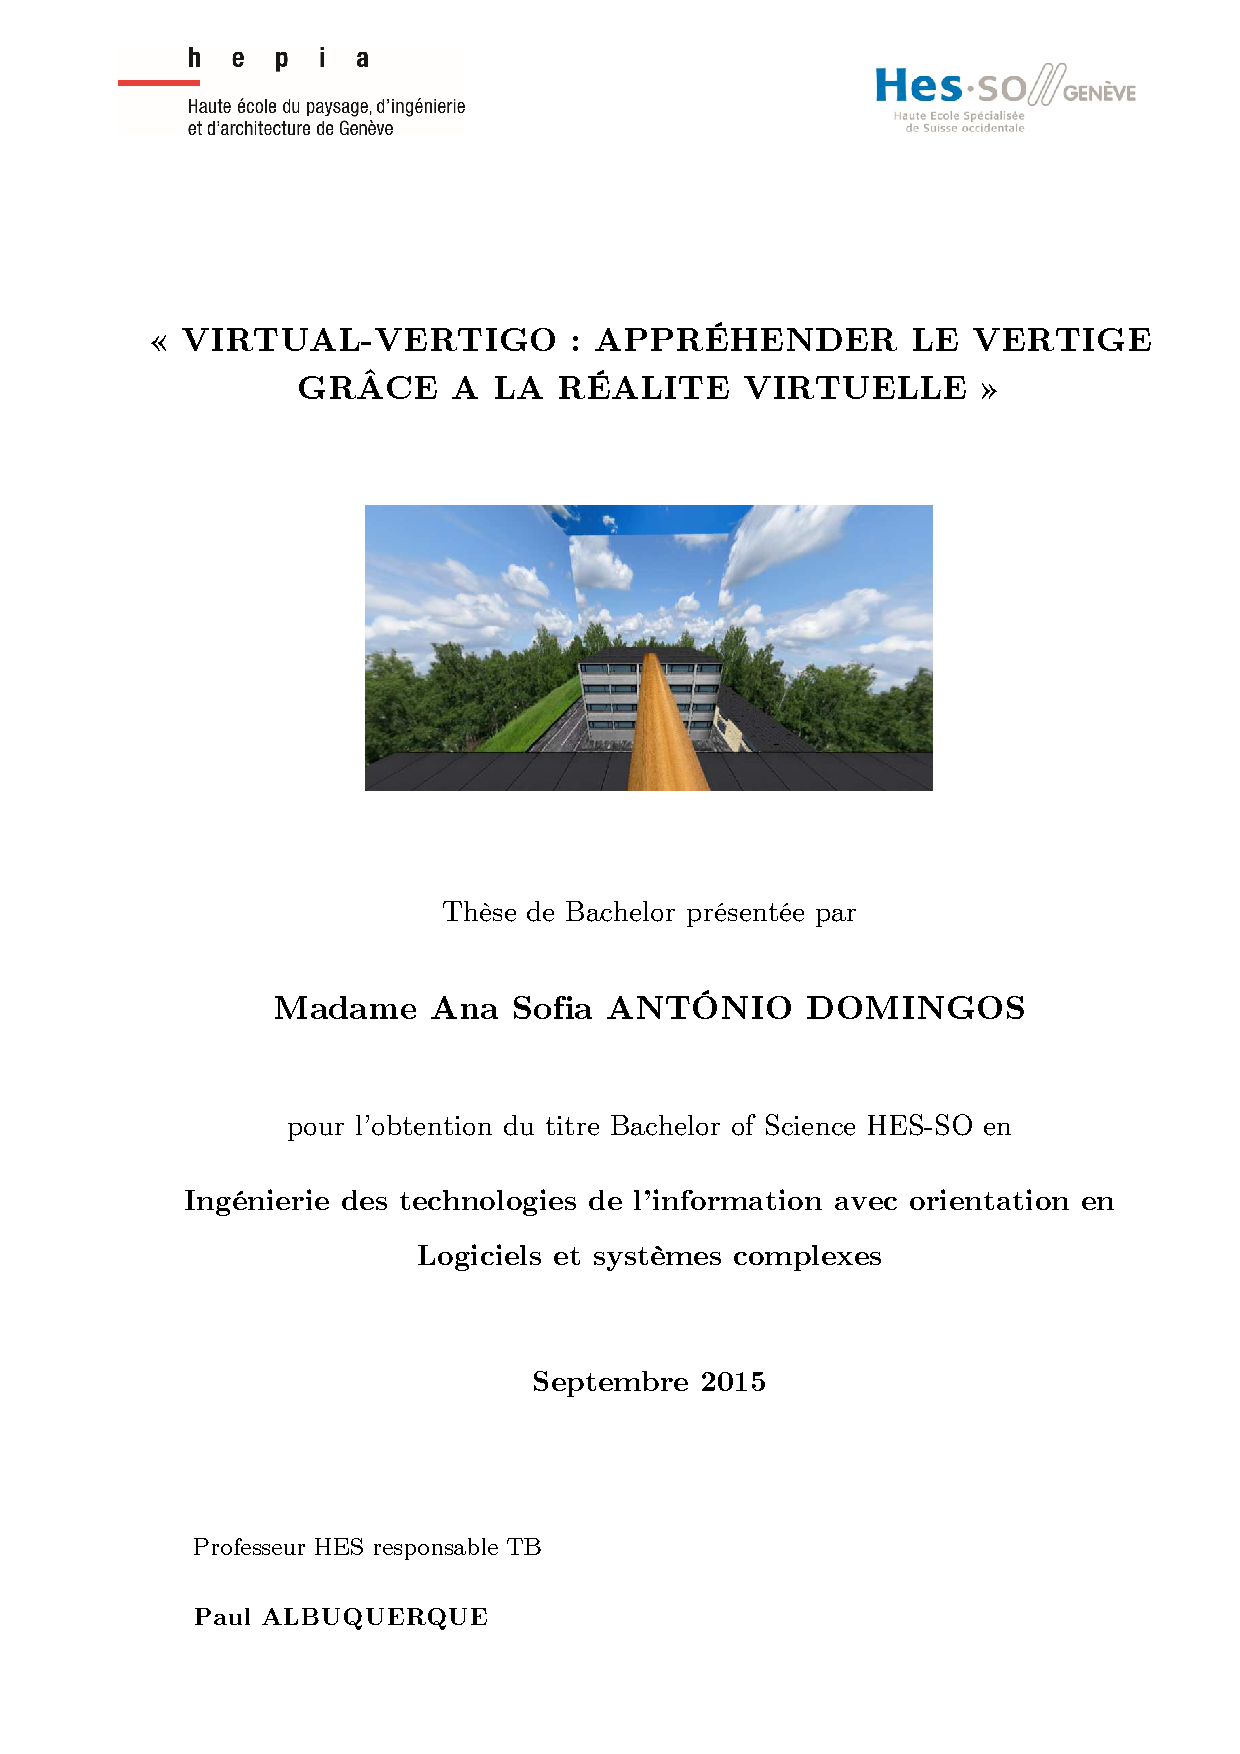
\includepdf[pages={1}]{Titre.pdf}
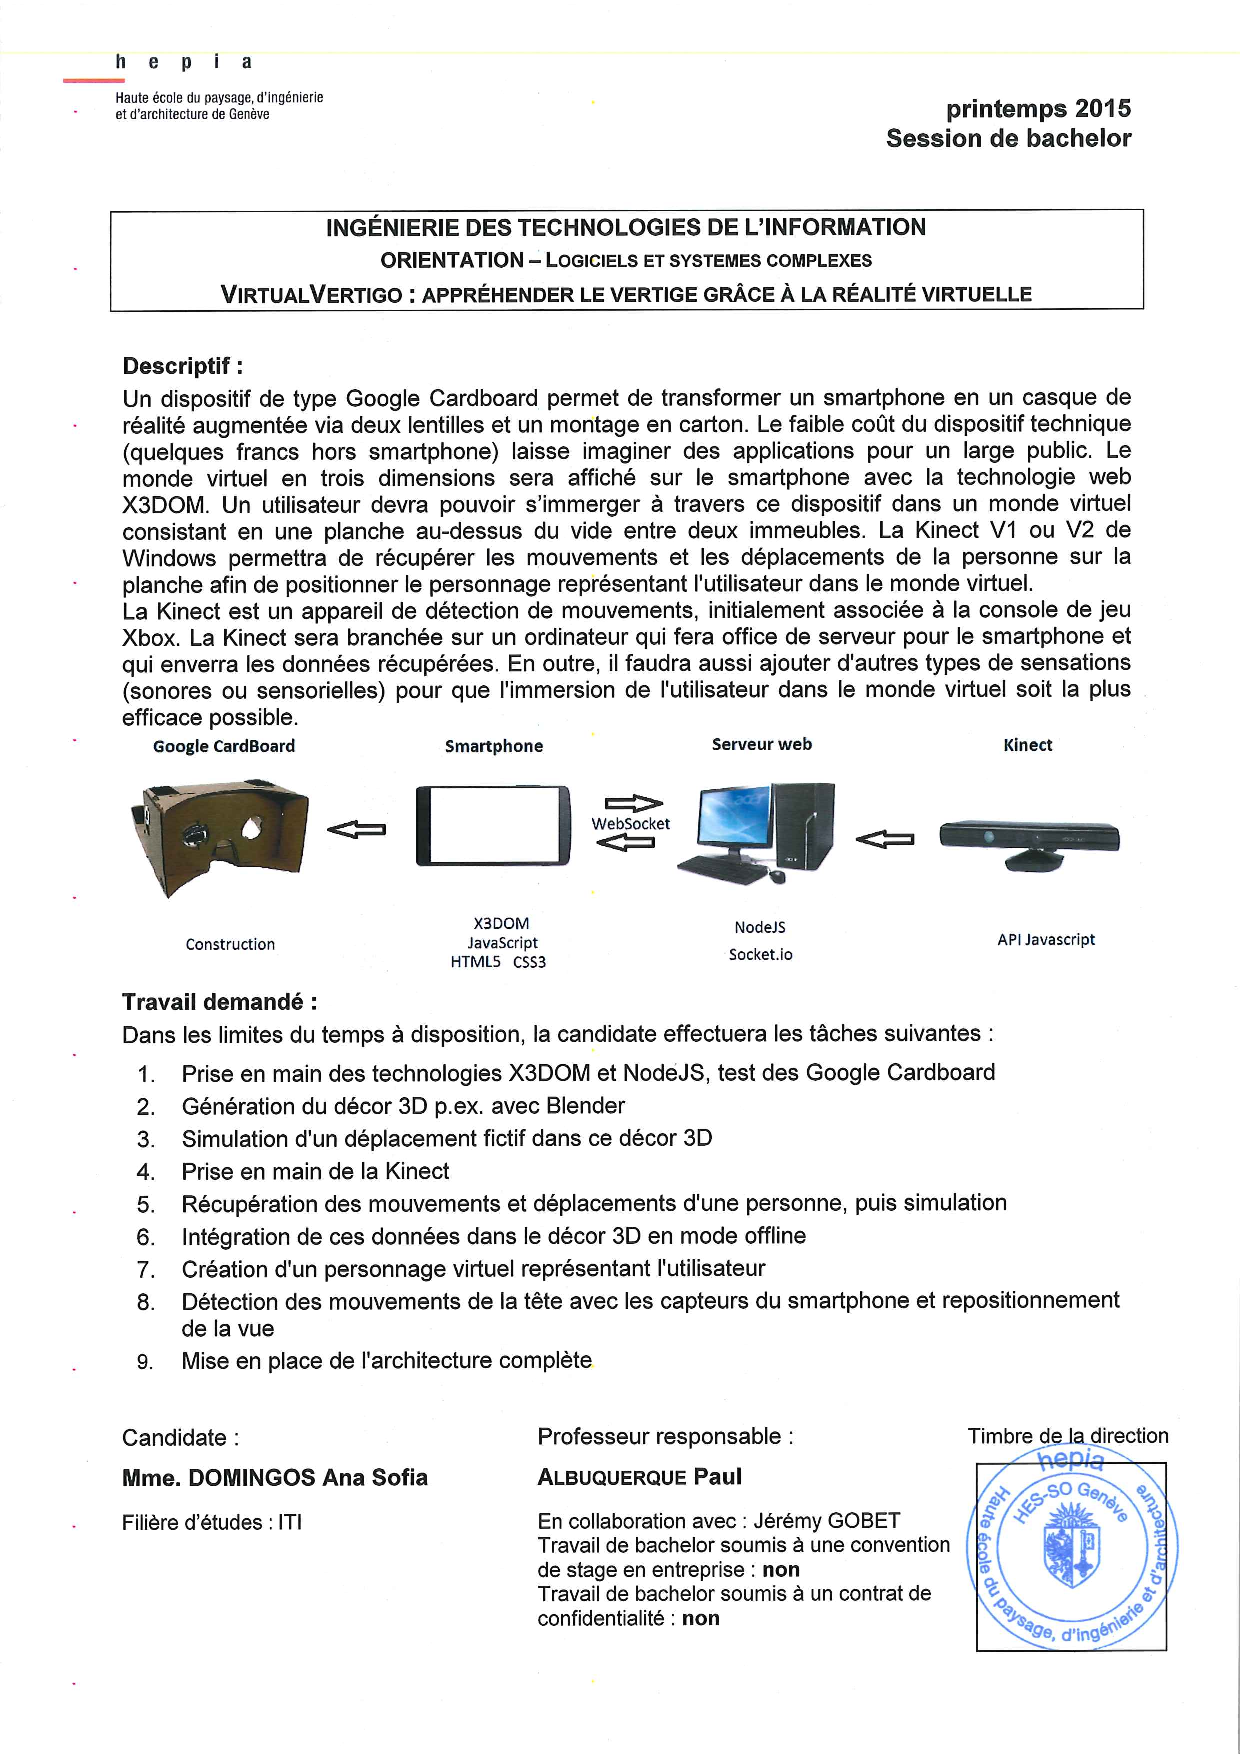
\includepdf[offset=0.8cm 0mm, pages={1}, width=20cm]{../reglement/ITI_IN_jour_enonce_diplome_Domingos_Albuquerque_2015.pdf}
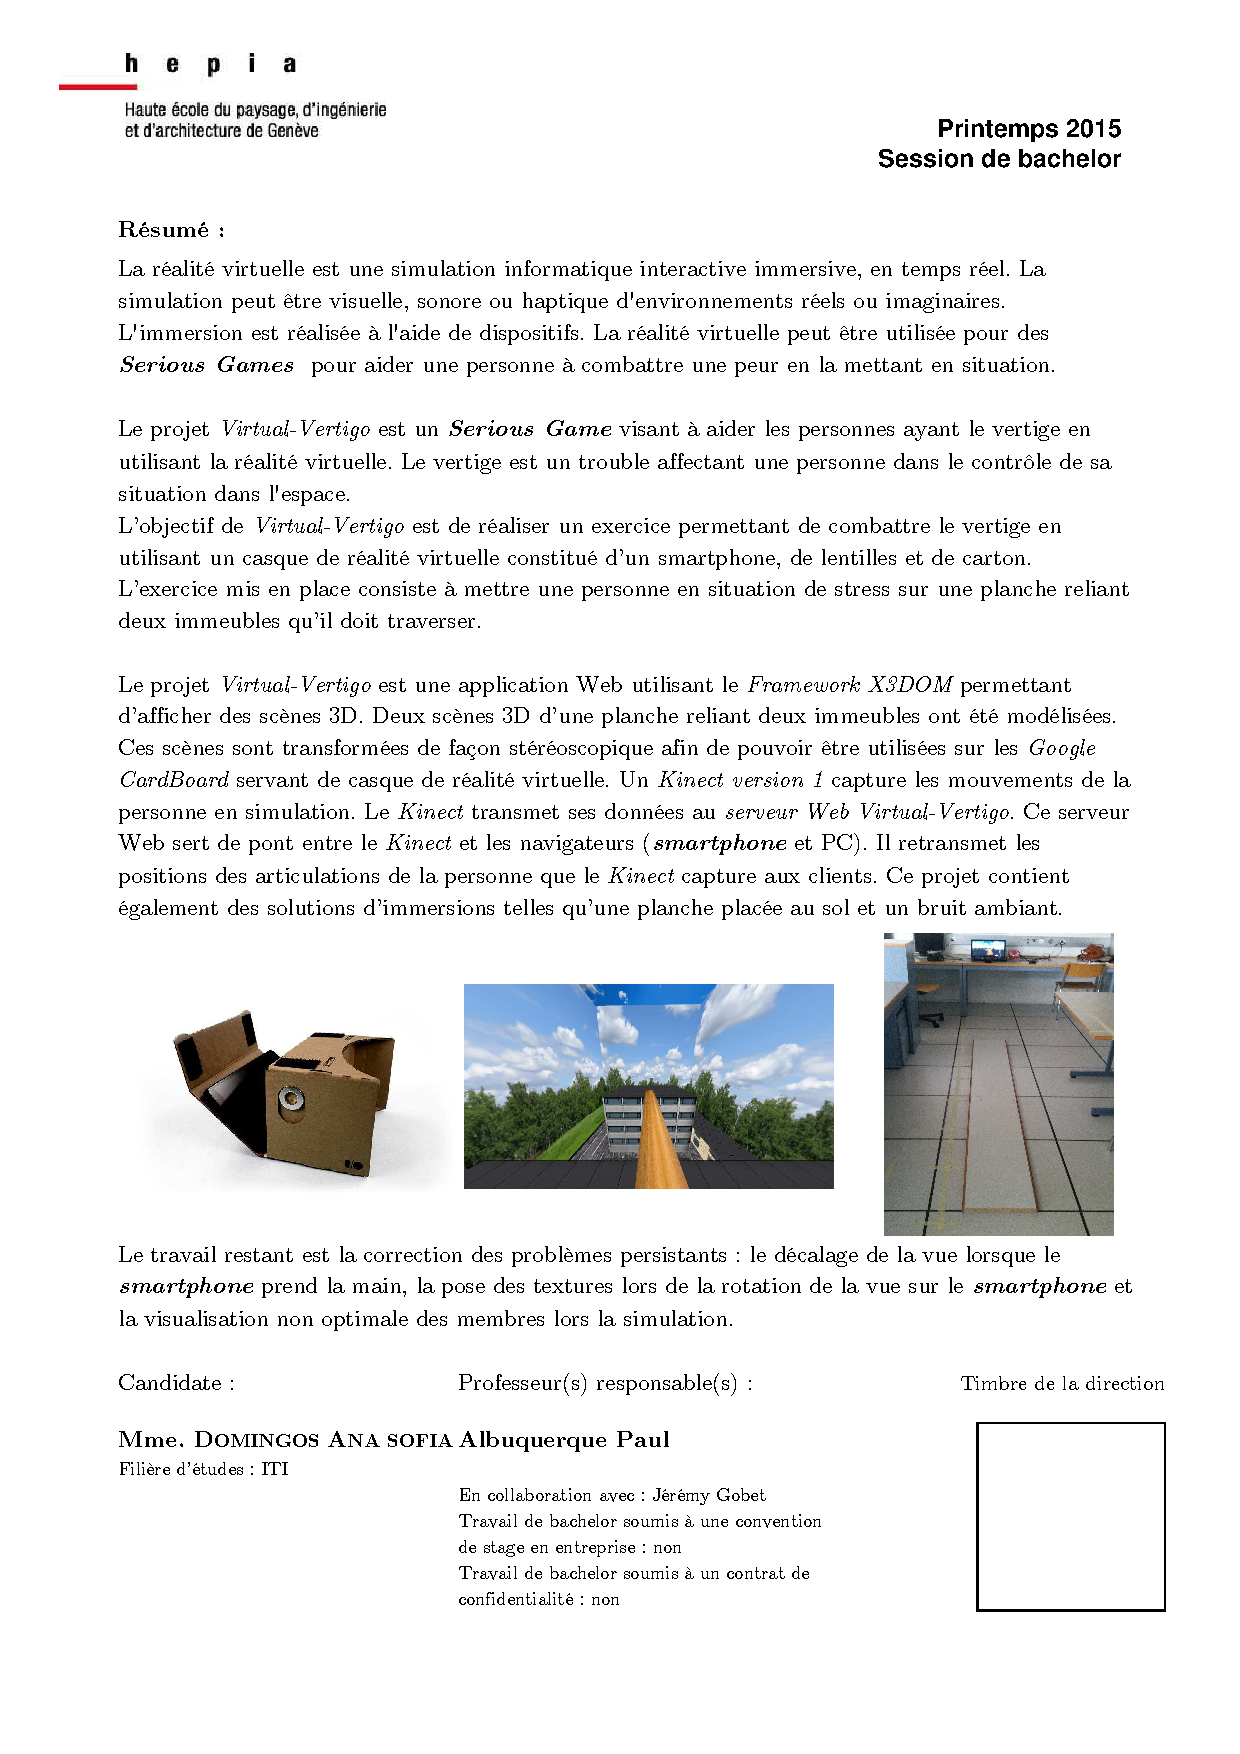
\includepdf[offset=0.8cm 0mm, pages={1}, width=20cm]{../documentation/Resume.pdf}
\section*{Avant propos}

Ce rapport décrit mon travail de Bachelor, réalisé sur une période de 12 semaines au sein de hepia. Le sujet de ce travail de Bachelor, a été proposé par \textsc{M. Jérémy Gobet} assistant à hepia à la filière ITI est l'implémentation du projet \textit{Virtual-Vertigo}. Ce projet consiste à mettre en place un exercice pour aider les personnes à combattre la peur du vide en utilisant la réalité virtuelle avec des casques de réalité virtuelle en carton et un smartphone. A noter que ce travail est la continuité de mon projet de semestre qui consistait à la prise en main, à la recherche et au choix des technologies et outils du projet \textit{Virtual-Vertigo}. 

\subsection*{Impressions personnelles}
Ce travail a été très intéressant, amusant et attractif à mettre en place. En effet, ce travail de Bachelor touche des domaines que j'apprécie énormément (développement \textit{Web} et \textit{3D}). L'implémentation du projet \textit{Virtual-Vertigo} a été agréable et importante car à chaque test de simulation, tout le monde voulait tester également. Il intéresse énormément de gens par son innovation. En effet, il vend du rêve : l'immersion totale dans un monde virtuel. Mon but était d'avoir une simulation opérationnelle même si elle contient encore quelques problèmes. J'ai hâte de le montrer au plus de monde possible et de travailler dans les domaines abordés dans ce travail. Ce fut une expérience très enrichissante et instructive. \\

J'espère que ce rapport et ce projet sera aussi intéressant pour vous qu'il a été pour moi de le mettre en place et de l'écrire.
\begin{center} Je vous souhaite une bonne lecture. \end{center} 
%%%%%%%%%%%%%%%%%%%%%%%%%%%%%%%%%%%%%%%%%%%%%%%%%%%%%%%%%%%%%%%%%%%%%%%%%%%%%%%%%%%%%%%%%%%%%%%%%%%%%%%%%%%%%%%%%%%%%%%%%%%
\subsection*{Informations}


\textbf{António Domingos Ana Sofia :} \href{ana.domingos@hotmail.fr}{ana.domingos@hotmail.fr}

Etudiante ITI travaillant sur le projet \textit{Virtual-Vertigo}

\textbf{Albuquerque Paul :} \href{paul.albuquerque@hesge.ch}{paul.albuquerque@hesge.ch}

Professeur à hepia dans la filière ITI reponsable

\textbf{Gobet Jérémy : }\href{jeremy.gobet@hesge.ch}{jeremy.gobet@hesge.ch}

Assistant à hepia dans la filière ITI ayant proposé le sujet et suivant également ce travail 

\subsection*{Suivi} 
Afin de permettre aux personnes suivant le projet de suivre l'avancement du \textit{Virtual-Vertigo} à tout moment, un dépôt \textit{GitHub} a été mis en place. \textit{GitHub} est un service Web d'hébergement et de gestion de développement de logiciels, utilisant le logiciel de gestion Git. Il propose un système de \textsf{versionning} (cela peut éviter les catastrophes) et un flux donnant la possibilité de partager et suivre des projets. \\
A noter que le dépôt \textit{GitHub} a été créé lors du travail de semestre et un serveur d'hébergement a été mis en place. Ce serveur a été mis en place parce qu'il était impossible de tester la réalité virtuelle localement. Un système de \textit{WebHook} a été ajouté à \textit{GitHub} afin de pouvoir mettre à jour le serveur hébergeant lors des changements sur le dépôt GitHub. \textit{WebHook} est une méthode permettant d'étendre, de personnaliser et d'intégrer une application Web lorsqu'un événement se produit (pour plus d'informations sur les \textit{WebHook}, voir \cite{webhook}).\\
A noter également que le \textit{WebHook} n'est plus utilisé durant le travail de Bachelor. En effet, un serveur \textit{Web} a pris la relais (pour plus d'informations sur ce serveur, voir la section~\ref{serveur}).

\newpage 

\section*{Remerciements}

Je tiens à remercier toutes les personnes qui m'ont aidé à la réalisation de ce travail de Bachelor. Plus particulièrement : \\

\textsc{M. Paul Albuquerque}, \textsc{M. Jérémy Gobet} et \textsc{M. Michaël Polla}, professeur et assistants à hepia à la filière ITI, pour m'avoir conseillé et aidé tout au long de la réalisation du projet \textit{Virtual-Vertigo}. \\

\textsc{M. Olivier Donzé} et \textsc{M. Benjamin Dupond-Roy}, professeur et assistant à hepia à la filière Architecture du paysage, pour m'avoir aidé et modélisé une scène de réalité virtuelle pour le projet \textit{Virtual-Vertigo}. \\

\textsc{M. Pascal Regamey}, assistant technique à hepia au département construction et environnement, pour avoir fournis la planche de 2.5 mètres pour la simulation de \textit{Virtual-Vertigo}. \\

Mes collègues de diplômes, pour m'avoir aidé à résoudre des problèmes, pour effectuer des simulations, pour m'avoir consacré du temps et pour la bonne humeur au cours de ce travail de diplôme.
\tableofcontents
\listoffigures
\bibliographystyle{unsrt}

\chapter{Introduction}
%%%%%%%%%%%%%%%%%%%%%%%%%%%%%%%%%%%%%%%%%%%%%%%%%%%%%%%%%%%%%%%%%%%%%%%%%%%%%%%%%%%%%%%%%%%%%%%%%%%%%%%%%%%%%%%%%%%%%%%%%%%
\section{Contexte}
La \textbf{réalité virtuelle} est une simulation informatique interactive immersive, en temps réel. Elle peut être constituée d'une simulation visuelle, sonore ou haptique d'environnements réels ou imaginaires. Le but de la réalité virtuelle est de permettre à une personne d'effectuer une activité sensori-motrice et cognitive dans un monde créé numériquement. L'immersion est réalisée à l'aide de dispositifs tels que des casques (\textit{OcculusRift} par exemple), des gants connectés, etc. \\
La réalité virtuelle peut être utilisée pour les \textsf{Serious Games} (voir~\cite{SeriousGame}). Le \textsf{Serious Game} est un logiciel combinant une intention "sérieuse" avec les jeux par exemple dans un contexte pédagogique ou de rééducation. Il a pour but de rendre attrayants les jeux ludiques. Par exemple, les \textsf{Serious Games} peuvent être utilisés pour la santé (le site LudoMedic~\cite{LudoMedic} du studio CCCP~\cite{cccp}).\\

Le projet \textit{Virtual-Vertigo} est un \textsf{Serious Game} mis en place afin d'aider les personnes à combattre le \textbf{vertige} en utilisant la réalité virtuelle.\\
Ce trouble affecte une personne dans le contrôle de sa situation dans l'espace. Il peut survenir dans différentes circonstances ou causes à tout âge. Plusieurs symptômes définissent le vertige : 
\begin{itemize}
\item une illusion de mouvements,
\item une impression de désorientation et déséquilibre,
\item une crise de panique,
\item bien d'autres.
\end{itemize}
A noter que les symptômes sont différents pour chaque personne. \\
Le vertige peut entraîner une phobie : l'acrophobie (la peur du vide). Cette phobie est une peur extrême et irrationnelle des hauteur. Les acrophobes souffrent de peur panique lorsqu'ils sont en hauteurs et veulent à tout prix redescendre. \\

Selon les spécialistes, le vertige et l'acrophobie se soignent généralement avec une psychothérapie. Cependant, depuis quelques années, ils commencent à faire des thérapies utilisant la réalité virtuelle. Cette thérapie permet aux personnes d'affronter leurs peurs. A noter que cette thérapie n'a pas encore fait ses preuves. En effet les résultats sont partiels et incertains (pour plus d'informations voir \cite{acrophobie}).

%%%%%%%%%%%%%%%%%%%%%%%%%%%%%%%%%%%%%%%%%%%%%%%%%%%%%%%%%%%%%%%%%%%%%%%%%%%%%%%%%%%%%%%%%%%%%%%%%%%%%%%%%%%%%%%%%%%%%%%%%%%

\section{Projet Virutal-Vertigo}
\textit{Virtual-Vertigo} est un projet de développement \textit{Web mobile 3D}. Le but de ce projet est de réaliser un exercice permettant de combattre la peur du vide. En utilisant des casques de réalité virtuelle en carton contenant un \textsf{smartphone} et des lentilles, l'exercice se déroule dans une réalité virtuelle modélisant la vue d'une planche reliant deux immeubles. La personne effectuant la simulation doit traverser cette planche afin d'atteindre l'immeuble d'en face.\\

Dans ce projet, on emploie un dispositif de \textit{Google CardBoard} pour réaliser le casque de réalité virtuelle. Le monde virtuel 3D sera affiché via la \textit{technologie Web X3DOM} qui permet d'afficher des scènes 3D dans un navigateur. Un utilisateur s'immerge à travers ce dispositif dans le monde virtuel en se déplaçant sur une planche reliant deux immeubles. Un \textit{Kinect} sera utilisé pour récupérer les mouvements et les déplacements de la personne afin de les reporter dans le monde virtuel. Le \textit{Kinect} doit être connecté à un serveur pour transmettre les données capturées aux navigateurs sur \textsf{smartphone} et PC. En outre, des solutions pour rendre l'immersion de l'utilisateur dans le monde virtuel plus réaliste seront abordées.

\begin{figure}[H]
\centering
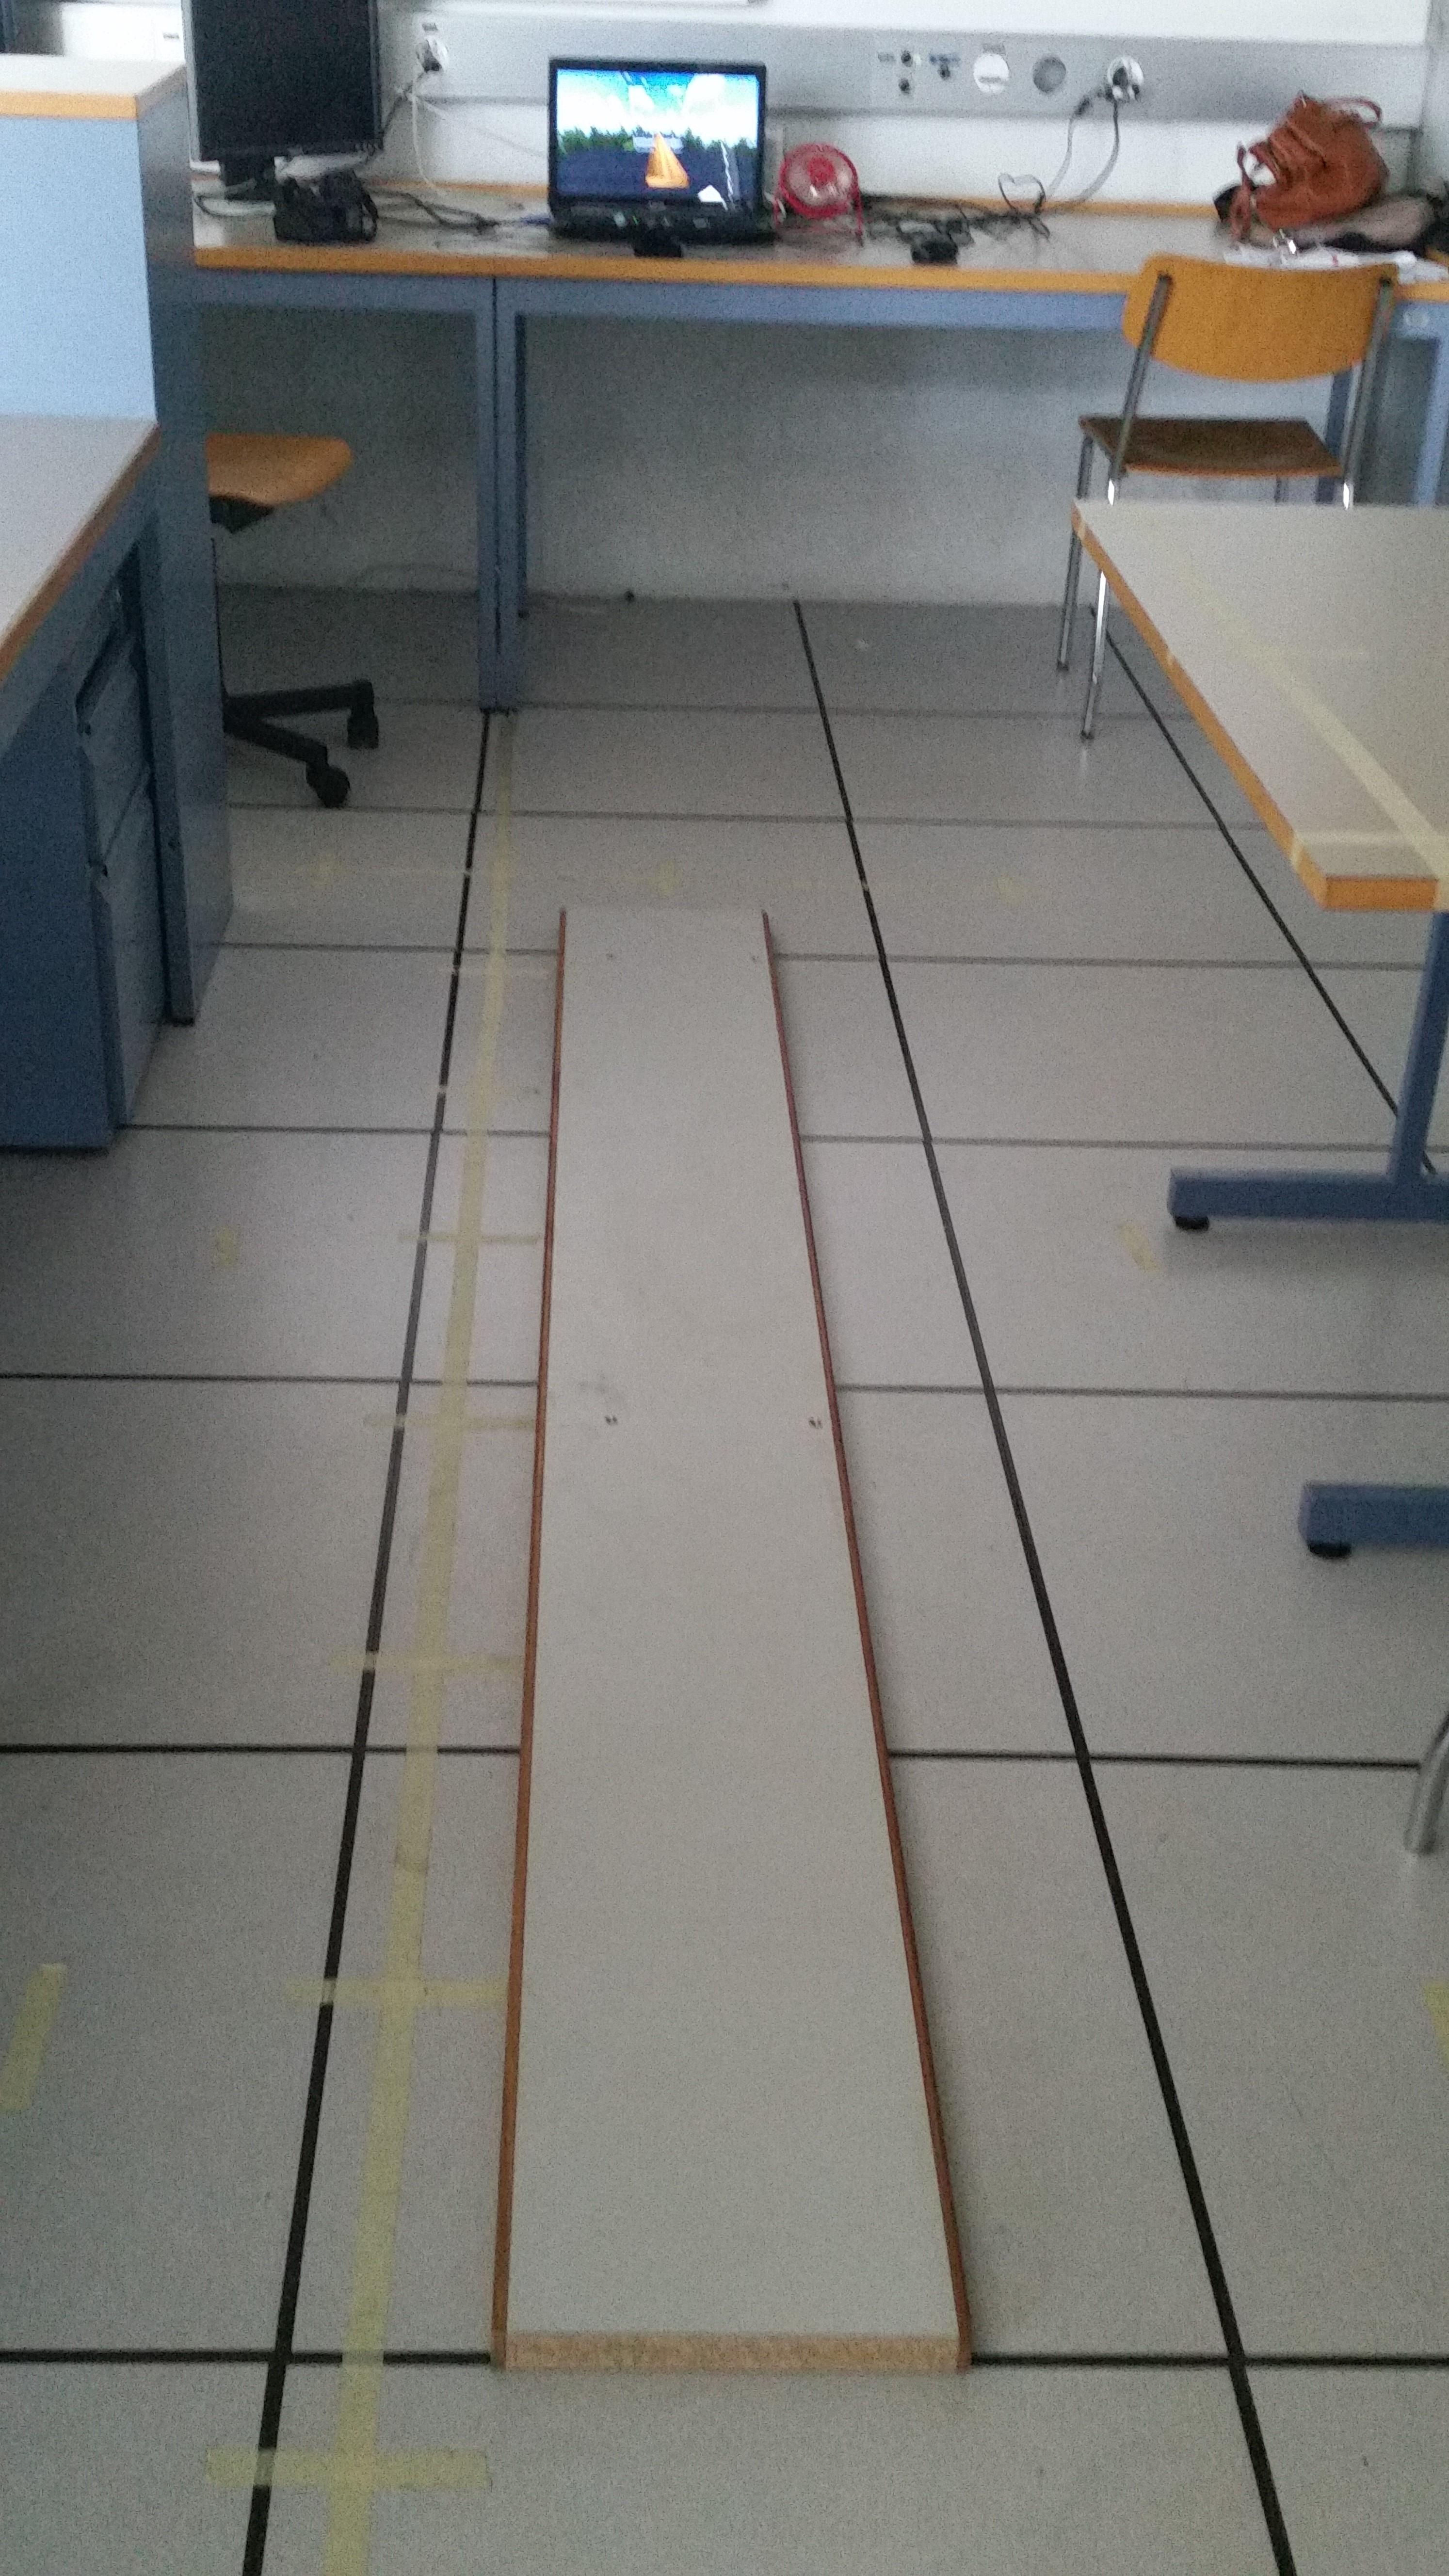
\includegraphics[scale=0.05]{vueReelle3.jpg}
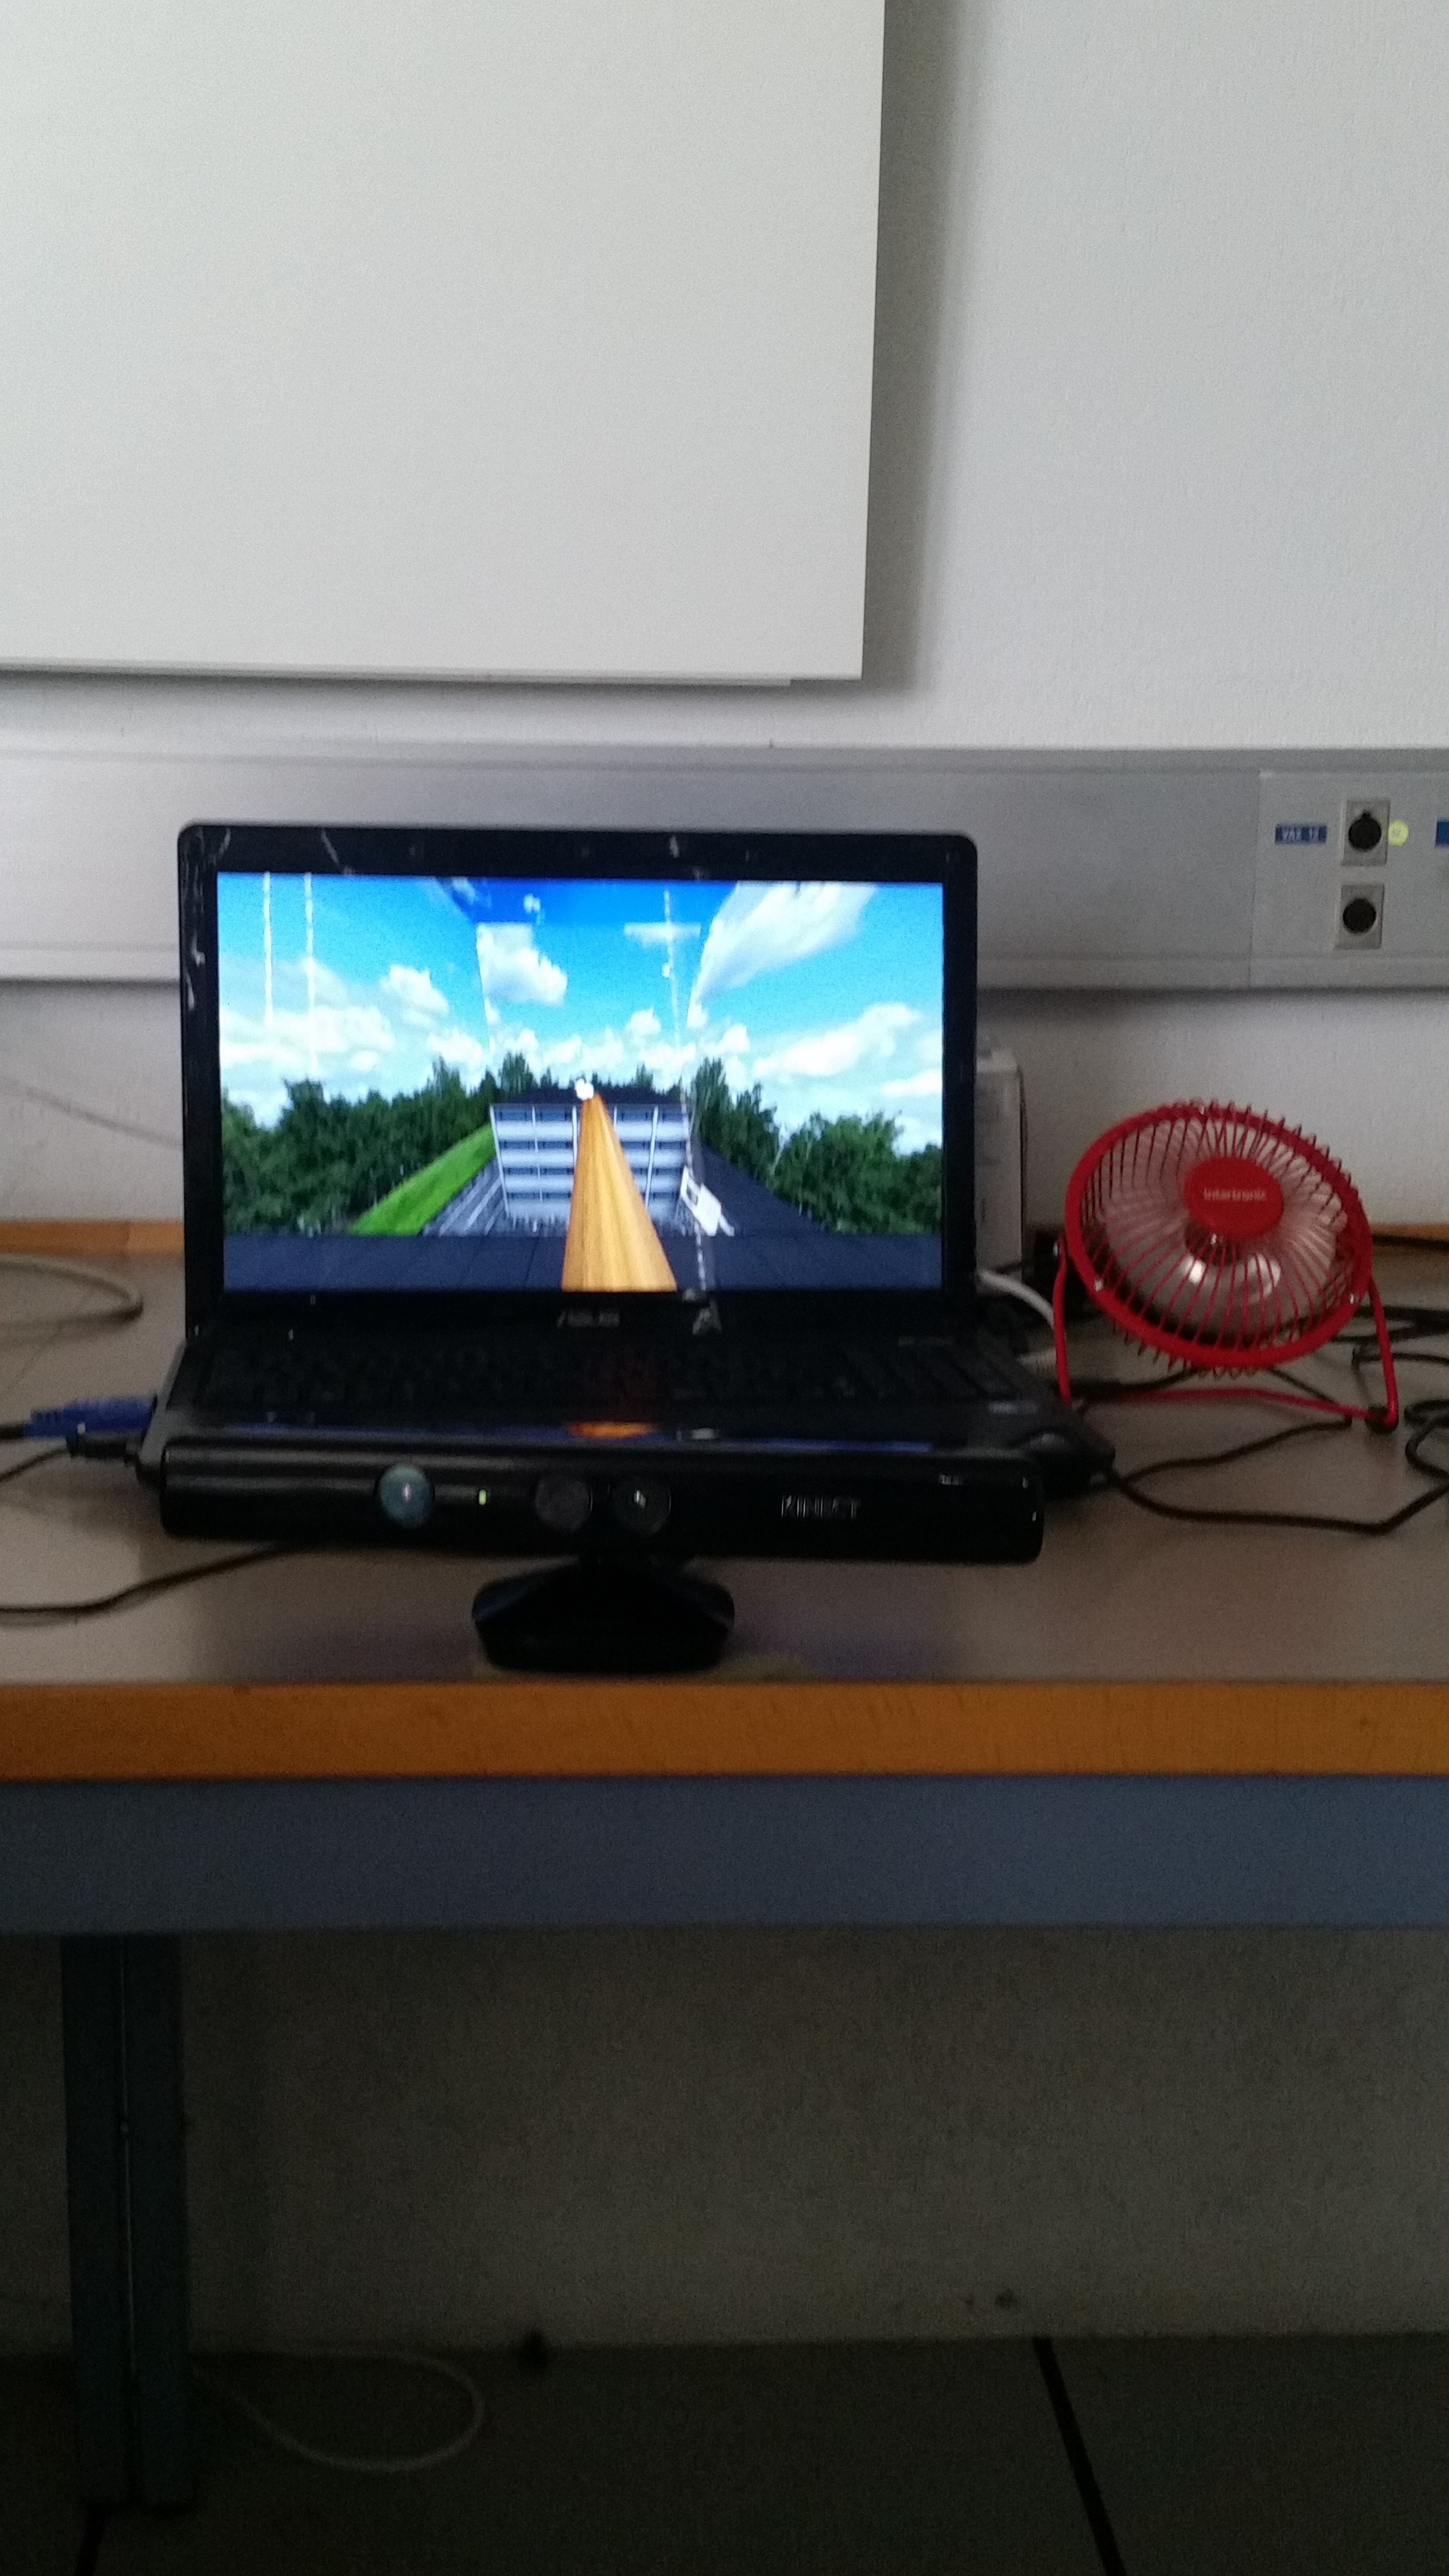
\includegraphics[scale=0.05]{vueReelle2.jpg}
\caption{\label{installation} Illustration de l'installation mise en place}
\end{figure}

La figure~\ref{installation} illustre l'installation mise en place pour le projet \textit{Virtual-Vertigo}.\\

A noter qu'un projet \textit{Ctrl Stress} développé par \textsc{M. Daniel Mestre}, psychologue et responsable du \textsf{Centre de Réalité Virtuelle de Méditerranée}, visant à vaincre la peur du vide avec la réalité virtuelle a déjà été mis en place a priori avec des \textit{Occulus Rift}. Pour lire un article sur ce projet, voir~\cite{cnrs}. Une étude~\cite{etude} a également été réalisée sur ce projet.\\
La principale différence entre \textit{Virtual-Vertigo} et \textit{Ctrl Stress} est que \textit{Virtual-Vertigo} permet à n'importe quelle personne possédant un \textit{Kinect} et des \textit{Google CardBoard} de l'utiliser alors que \textit{Ctrl Stress} n'est pas disponible. De plus le dispositif de \textit{Crtl Stress} est probablement cher.\\

A noter également qu'un glossaire décrivant toutes les technologies et les outils utilisés dans le projet \textit{Virtual-Vertigo} est disponible en annexe~\ref{glossaire}.

%%%%%%%%%%%%%%%%%%%%%%%%%%%%%%%%%%%%%%%%%%%%%%%%%%%%%%%%%%%%%%%%%%%%%%%%%%%%%%%%%%%%%%%%%%%%%%%%%%%%%%%%%%%%%%%%%%%%%%%%%%%

\section{Organisation du projet}
Le projet \textit{Virtual-Vertigo} dans son intégralité a été séparé en deux parties : 
\begin{enumerate}
\item Le \textsf{projet de semestre} était d'une durée équivalente à 3 semaines à temps complet, réparties sur un semestre. A la suite de ce travail, les bases du projet ont été mises en place :
\begin{itemize}
\item la construction des \textit{Google CardBoard},
\item la modélisation d'une vue basique 3D,
\item l'adaptation de la vue aux lunettes (stéréoscopie),
\item le choix entre les différentes technologies possibles pour l'échange et la capture des données,
\item la rotation d'un objet dans la vue 3D en fonction du smartphone,
\item le choix du \textit{Kinect} utilisé,
\item une rapide prise en main du \textit{Kinect}. \\

\end{itemize}

\item Lors du \textsf{travail de Bachelor} d'une durée de 12 semaines à temps complet, les éléments suivant ont été réalisés selon des plannings en annexe~\ref{plannings} :
\begin{itemize}
\item la modélisation de la vue finale (section~\ref{immeubles}~et~\ref{textures}),
\item le partage des données entre les outils (\textit{Kinect}, serveur et clients HTML) (section~\ref{serveur}~et~\ref{serveur2}),
\item la création du personnage virtuel (section~\ref{personnages}),
\item le déplacement de la personne dans la réalité virtuelle en fonction de la position de la tête (section~\ref{avancement}),
\item l'animation des membres de la personne dans la réalité virtuelle (section~\ref{animationPersonnage}),
\item l'adaptation de la vue sur le smartphone en fonction de la rotation de la tête (section~\ref{orientation}),
\item l'ajout de solutions pour une immersion plus réaliste (section~\ref{realisme}).
\end{itemize}

\end{enumerate}

\chapter{Virtual-Vertigo} \label{vertigo}
Ce chapitre décrit de manière plus détaillée le projet \textit{Virtual-Vertigo}. Il est séparé en deux parties distinctes, un descriptif du dispositif et la présentation de  l'architecture de l'application. Ces parties sont illustrées afin d'en faciliter la compréhension.

%%%%%%%%%%%%%%%%%%%%%%%%%%%%%%%%%%%%%%%%%%%%%%%%%%%%%%%%%%%%%%%%%%%%%%%%%%%%%%%%%%%%%%%%%%%%%%%%%%%%%%%%%%%%%%%%%%%%%%%%%%%

\section{Dispositif} \label{dispositif}

Le projet \textit{Virtual-Vertigo} aide une personne à combattre sa peur du vide en utilisant la réalité virtuelle. Pour cela, cette personne portera un casque de réalité virtuelle constitué d'un téléphone et d'un support en carton comprenant des lentilles. Ce dispositif permet l'affichage d'une scène virtuelle 3D via des images stéréoscopiques. \\
Lors de la simulation, l'utilisateur devra avancer sur une planche placée au sol. Un appareil posé sur une table face à la planche permettra de capturer ses mouvements. L'appareil connecté à un serveur devra transmettre les informations de positions au téléphone. Un affichage sur un écran standard donnera aussi une autre vue de la scène.\\

Voici quelques images illustrant la vue de la scène :
\begin{figure}[H]
   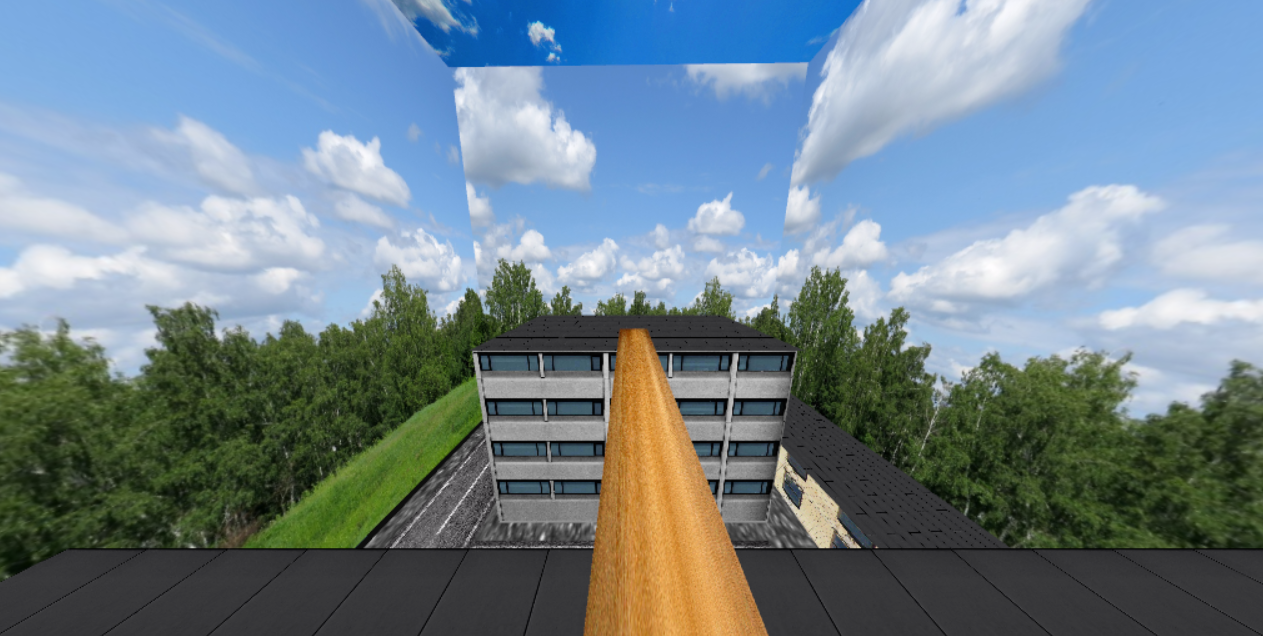
\includegraphics[scale=0.202]{vueBasiqueTextures.png}
   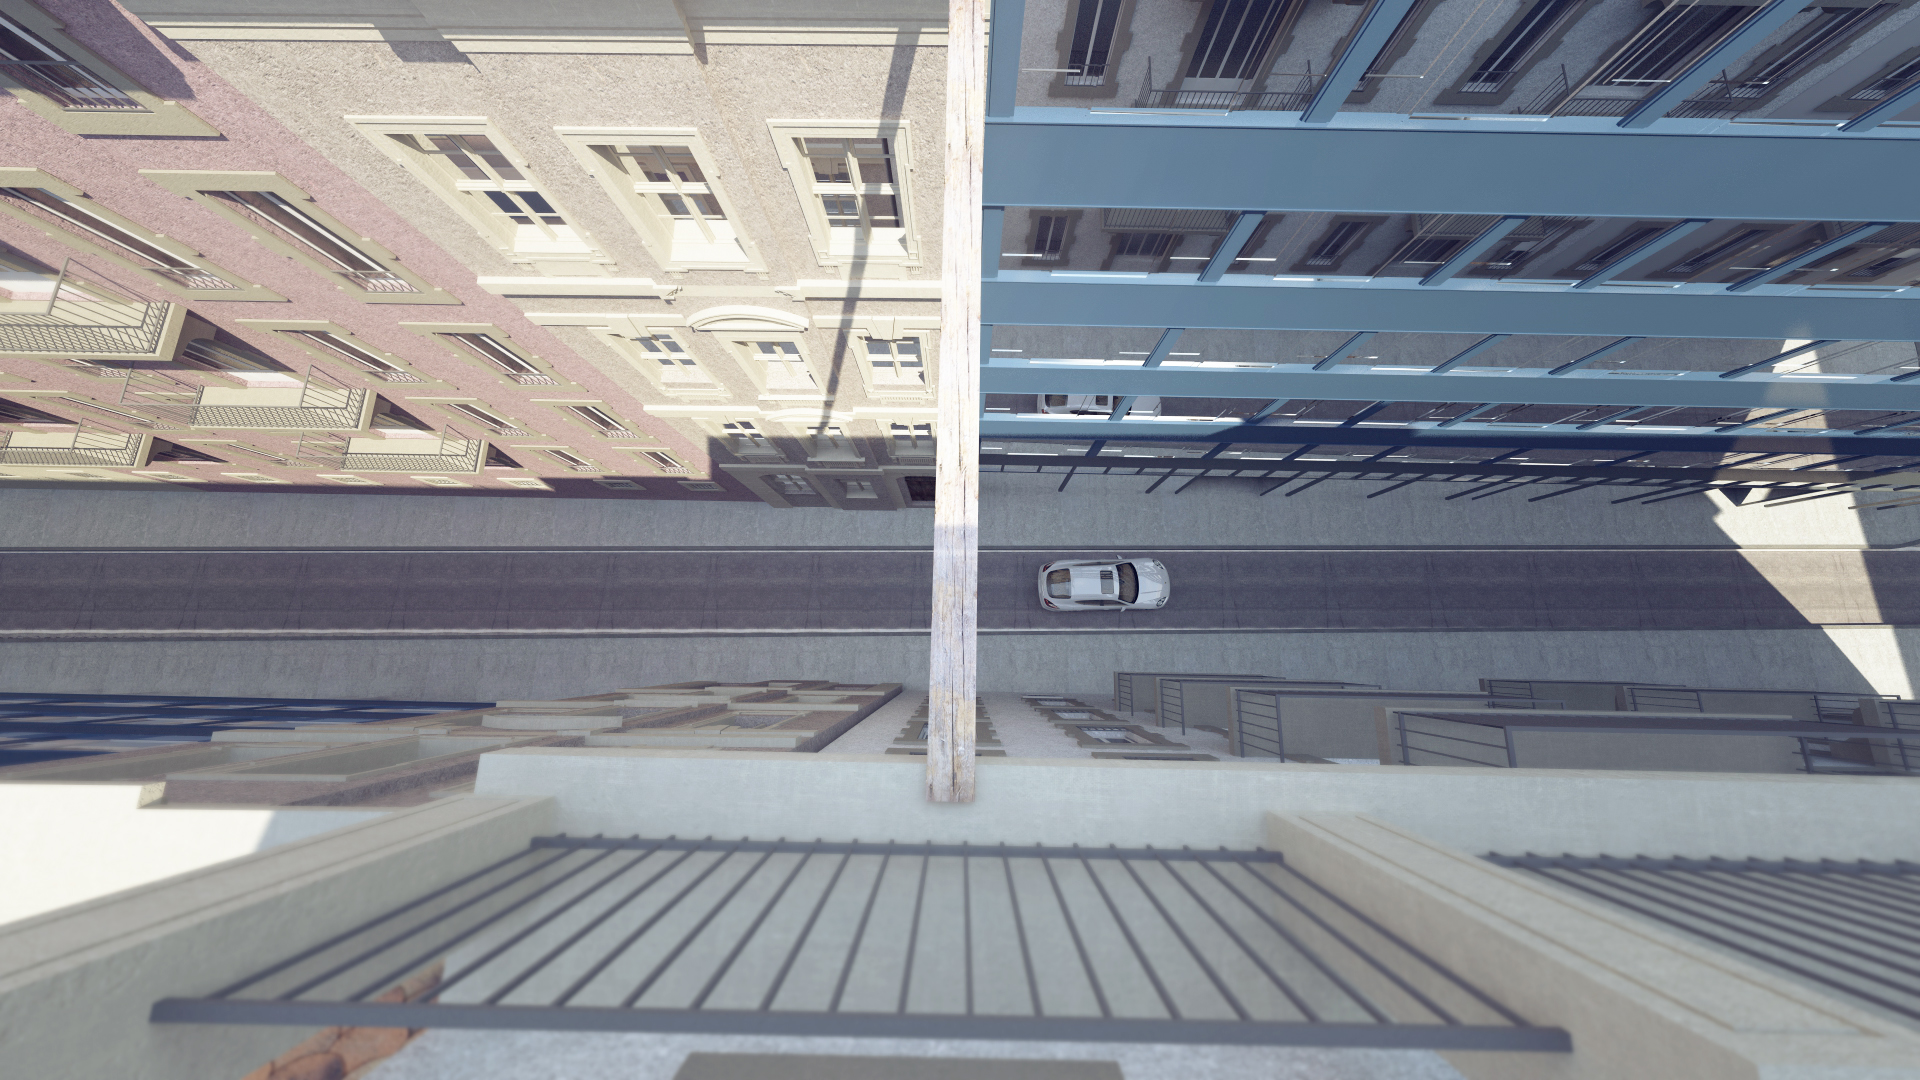
\includegraphics[scale=0.09]{Vue_planche2_ok.jpg}
   \caption{\label{vue} Vue 3D vue par la personne portant les lunettes}
\end{figure}

La deuxième image a été produite par \textsc{M. Benjamin Dupond-Roy}, assistant à hepia en filière architecture du paysage. Plus d'informations sont disponibles quant à la construction de ces images à la section~\ref{realiteVirtuelle}.

A noter qu'un tutoriel contenant les instructions pour l'installation et l'utilisation du projet \textit{Virtual-Vertigo} est disponible en annexe.

%%%%%%%%%%%%%%%%%%%%%%%%%%%%%%%%%%%%%%%%%%%%%%%%%%%%%%%%%%%%%%%%%%%%%%%%%%%%%%%%%%%%%%%%%%%%%%%%%%%%%%%%%%%%%%%%%%%%%%%%%%%

\subsection*{Composants} \label{composants}
Ci-dessous se trouve la liste des appareils et logiciels utilisés dans le projet : 

\begin{itemize}
\item \textbf{une Google CardBoard} : il s'agit du casque de réalité virtuelle en carton et équipé de lentilles;
\item \textbf{un smartphone} : il s'agit de l'appareil qui permet la visualisation en 3D stéréoscopique;
\item \textbf{un Kinect version 1} : c'est l'appareil qui détecte les mouvements de la personne sur la planche; 
\item \textbf{Kinect SDK 1.8} : c'est le logiciel permettant d'utiliser le \textit{Kinect} à partir d'un ordinateur;
\item \textbf{NodeJS} : c'est le \textit{Framework JavaScript} permettant de créer et lancer le serveur qui gère les transmissions entre le \textit{Kinect} et les clients HTML (\textsf{smartphone}, PC, etc.);
\item \textbf{un ordinateur sur Windows 7 ou plus} : il s'agit du serveur sur lequel est connecté le \textit{Kinect}. \\

\end{itemize}

Le schéma suivant illustre l'interaction entre les composants mentionnés ci-dessus. Sous chaque composant se trouvent les technologies qu'il utilise.\\

\begin{figure}[H]
	\centering
   		\includegraphics[scale=0.3]{description.png}
   \caption{\label{Schéma} Schéma du projet et de ses composants}
\end{figure}

La description de chaque composant est donnée au chapitre~\ref{implementation}. \\
A noter également qu'un glossaire décrivant toutes les technologies et les outils utilisés dans le projet \textit{Virtual-Vertigo} est disponible en annexe.

\subsubsection{Prix des composants}
Les seuls composants devant être achetés sont le \textit{Kinect} et les \textit{Google CardBoard}, le \textsf{smartphone} n'est pas pris en compte dans la liste des achats car tout le monde en possède un. Voici un tableau des prix :

\begin{center}
	\begin{tabular}{| c | c |}
	\hline
		\textbf{Composant} & \textbf{Prix} \\ \hline
		Kinect v1 pour Windows & 150 CHF \\ \hline
		Google CardBoard à assembler & 11 CHF \\ \hline
		Matériel pour les Google CardBoard & 11 CHF \\ \hline
		Kinect v2 + adaptateur pour Windows & 180 CHF \\ \hline
		Occulus Rift & entre 300 et 400 CHF\\ \hline
	\end{tabular} 
	\captionof{table}{\label{prix}Tableau prix des composants}
\end{center}

Le tableau~\ref{prix} montre que le prix total des composants nécessaires au projet \textit{Virtual-Vertigo} est de moins de 200 CHF. Si l'\textit{Occulus Rift} avait été utilisé au lieu des \textit{Google CardBoard} le prix du projet aurait triplé. Le prix des \textit{Occulus Rift} est économisé. 

%%%%%%%%%%%%%%%%%%%%%%%%%%%%%%%%%%%%%%%%%%%%%%%%%%%%%%%%%%%%%%%%%%%%%%%%%%%%%%%%%%%%%%%%%%%%%%%%%%%%%%%%%%%%%%%%%%%%%%%%%%%
\subsection*{Disposition générale des composants} \label{disposition}
Le projet utilise beaucoup de composants qui doivent être positionnés de manière précise. Le schéma suivant montre l'emplacement de chaque composant.

\begin{figure}[H]
	\centering
   		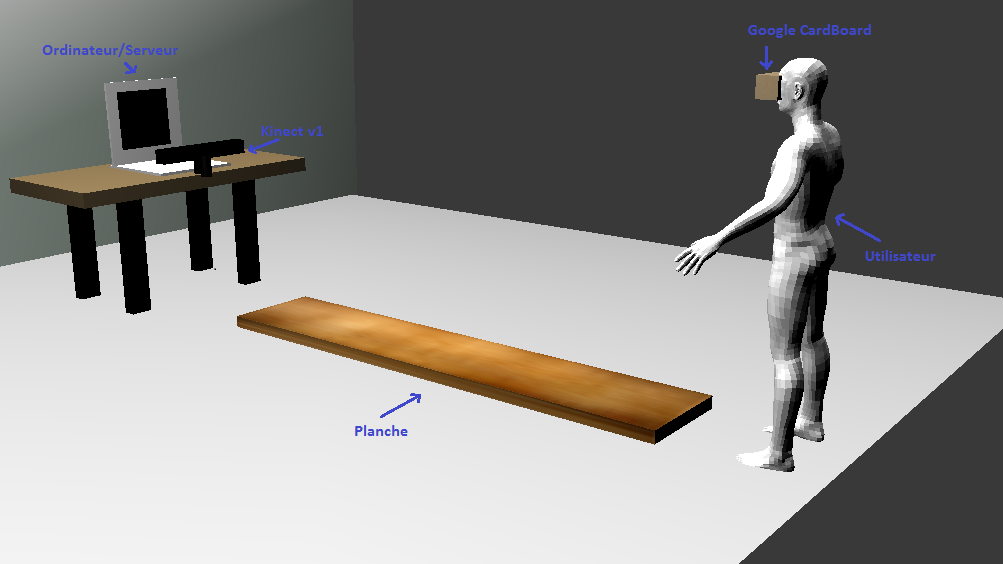
\includegraphics[scale=0.5]{vertigo.png}
   	\caption{\label{vertigo} Modèle 3D de l'installation de \textit{Virtual-Vertigo}}
\end{figure}

Ce schéma ne montre cependant pas les restrictions imposées par le \textit{Kinect}: 
\begin{itemize}
\item la planche placée sur le sol ne peut pas faire plus de 3 mètres;
\item la planche doit être placée à une distance d'au moins 80 centimètres du \textit{Kinect};
\item l'utilisateur doit se trouver à une distance de moins de 4 mètres du \textit{Kinect};
\item le \textit{Kinect} doit être placé au bord de la table afin d'éviter qu'il ne capte pas les membres inférieurs de l'utilisateur ;
\item le \textit{Kinect} doit être connecté en USB à l'ordinateur. \\

\end{itemize}

A noter que le \textsf{smartphone} est connecté en wifi ou 3G au serveur. Il est intégré aux \textit{Google CardBoard} et affiche chacune des deux images stéréoscopiques que l'utilisateur visualise à travers les lentilles.\\

Les photos~\ref{reelle} sont l'installation réelle mise en place durant le développement du projet \textit{Virtual-Vertigo}.
\begin{figure}[H]
\centering
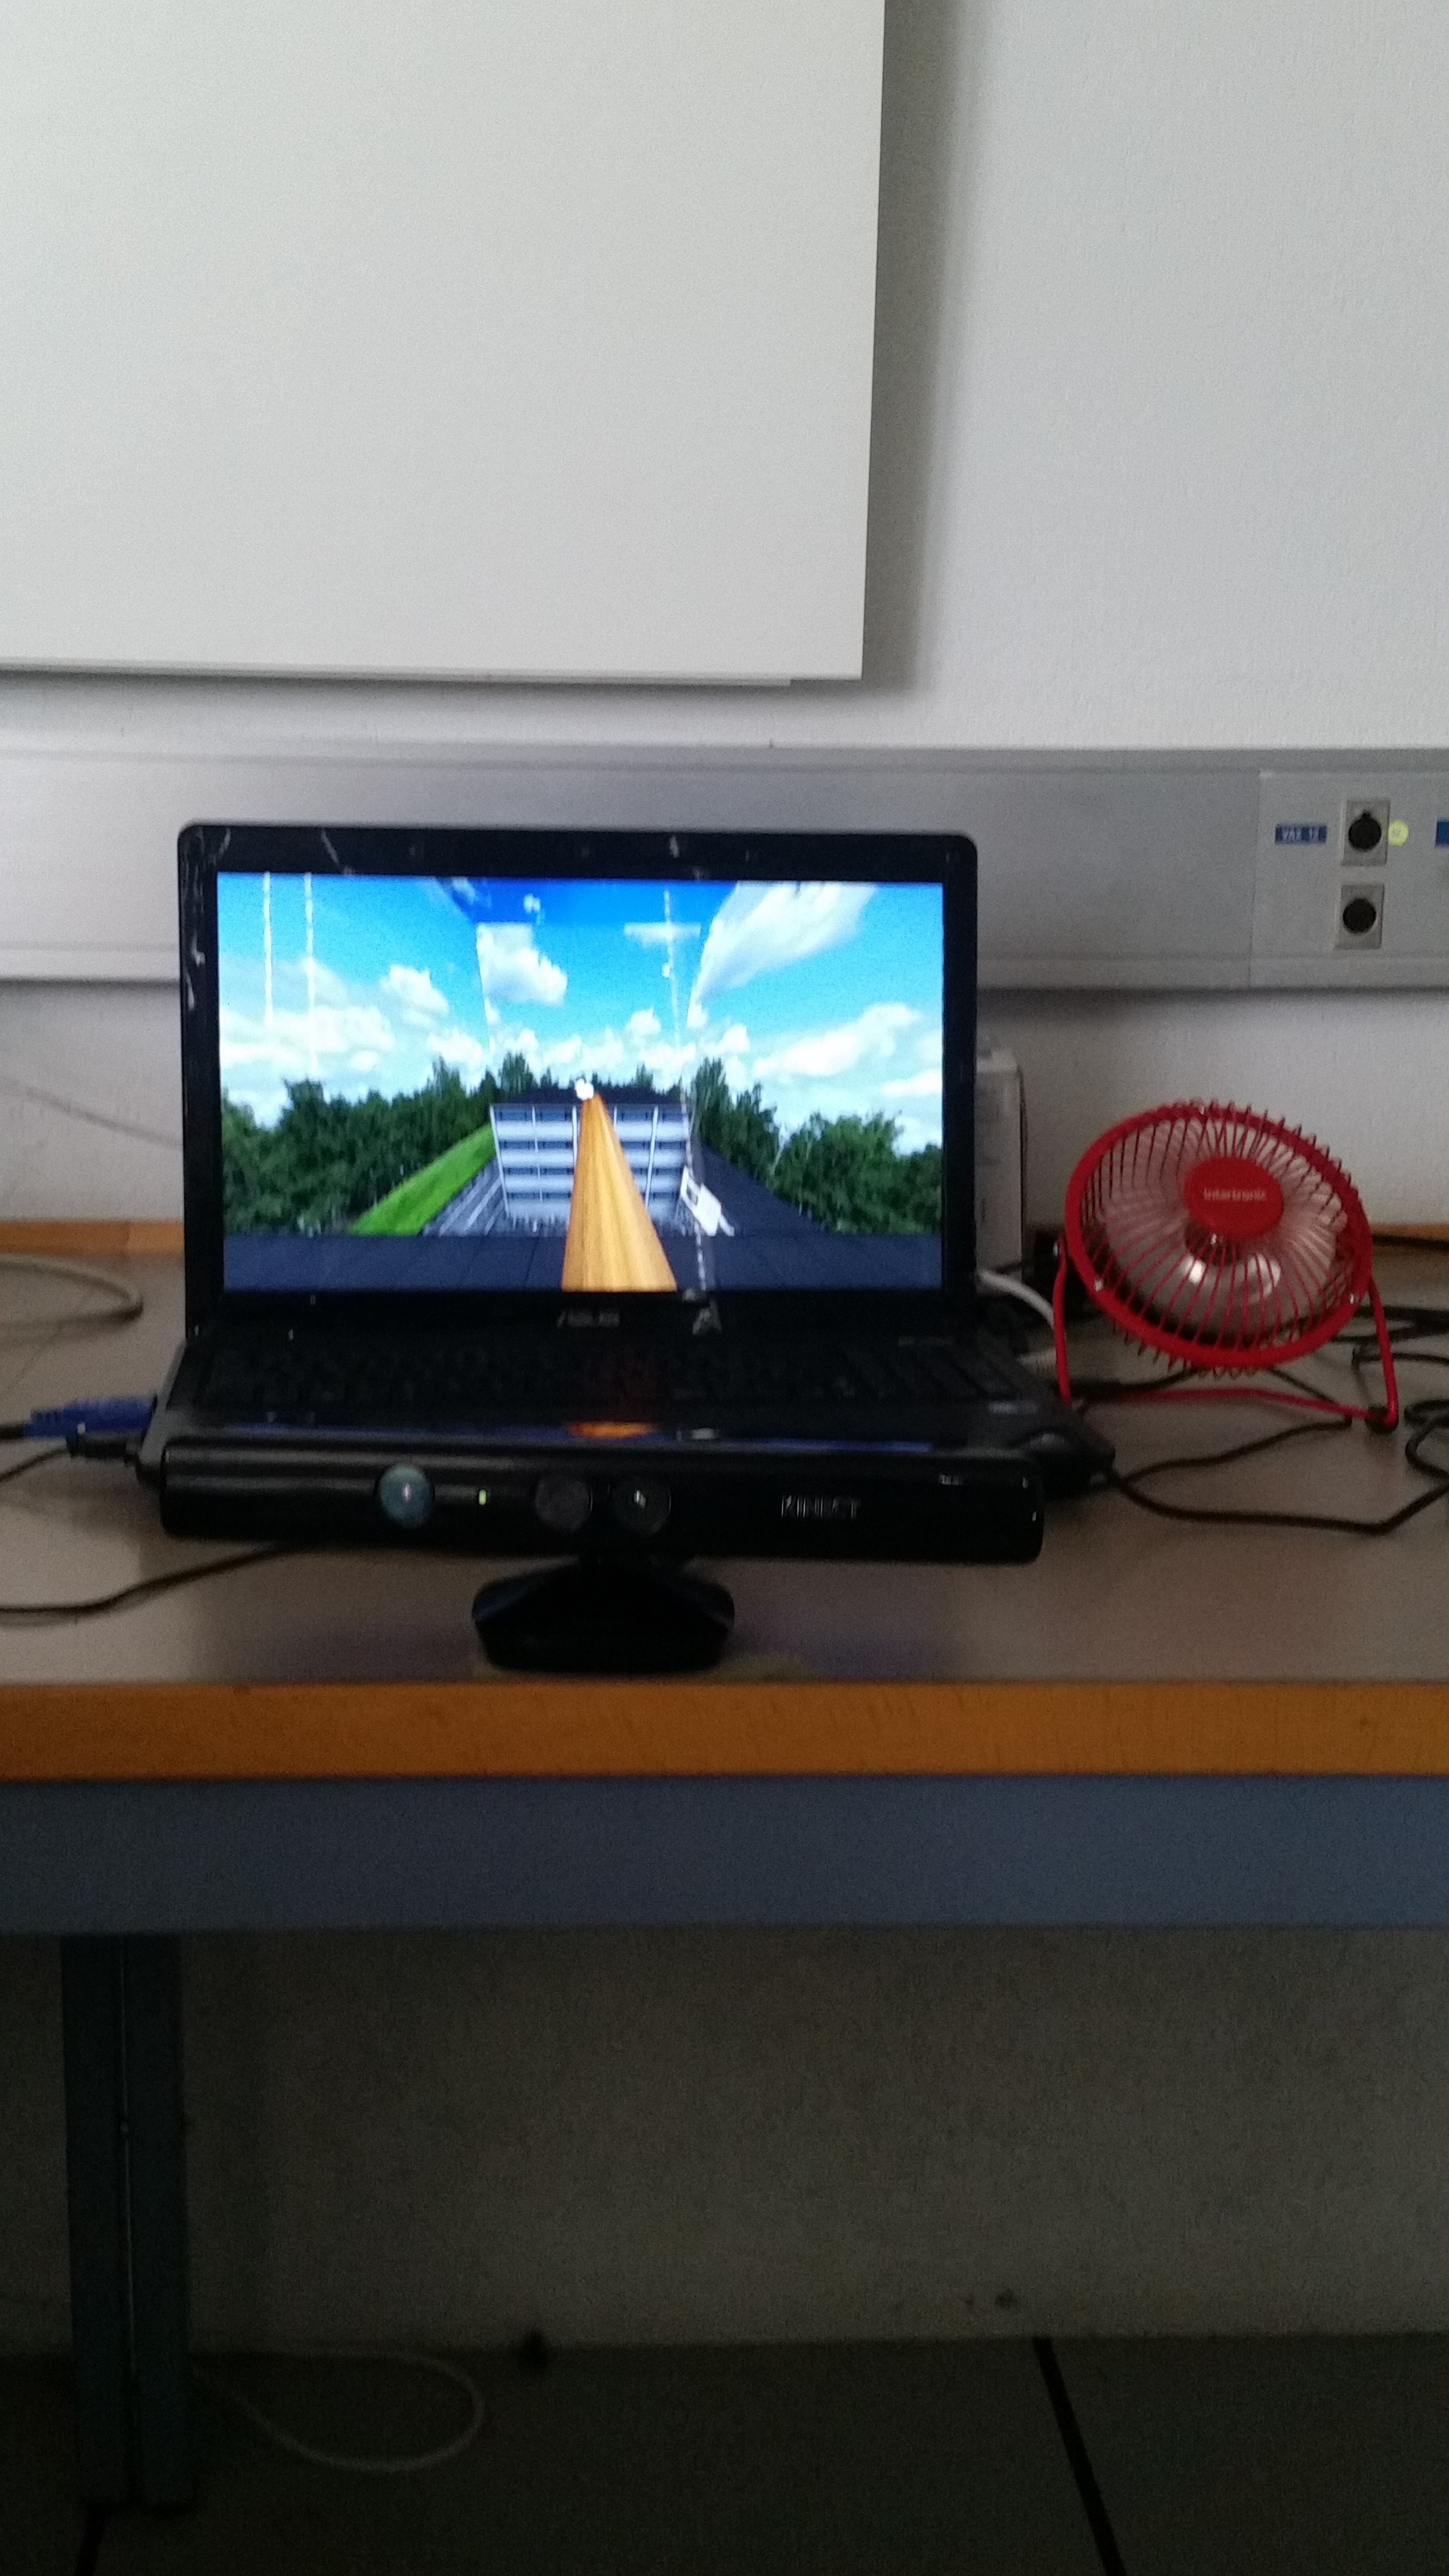
\includegraphics[scale=0.04]{vueReelle2.jpg}
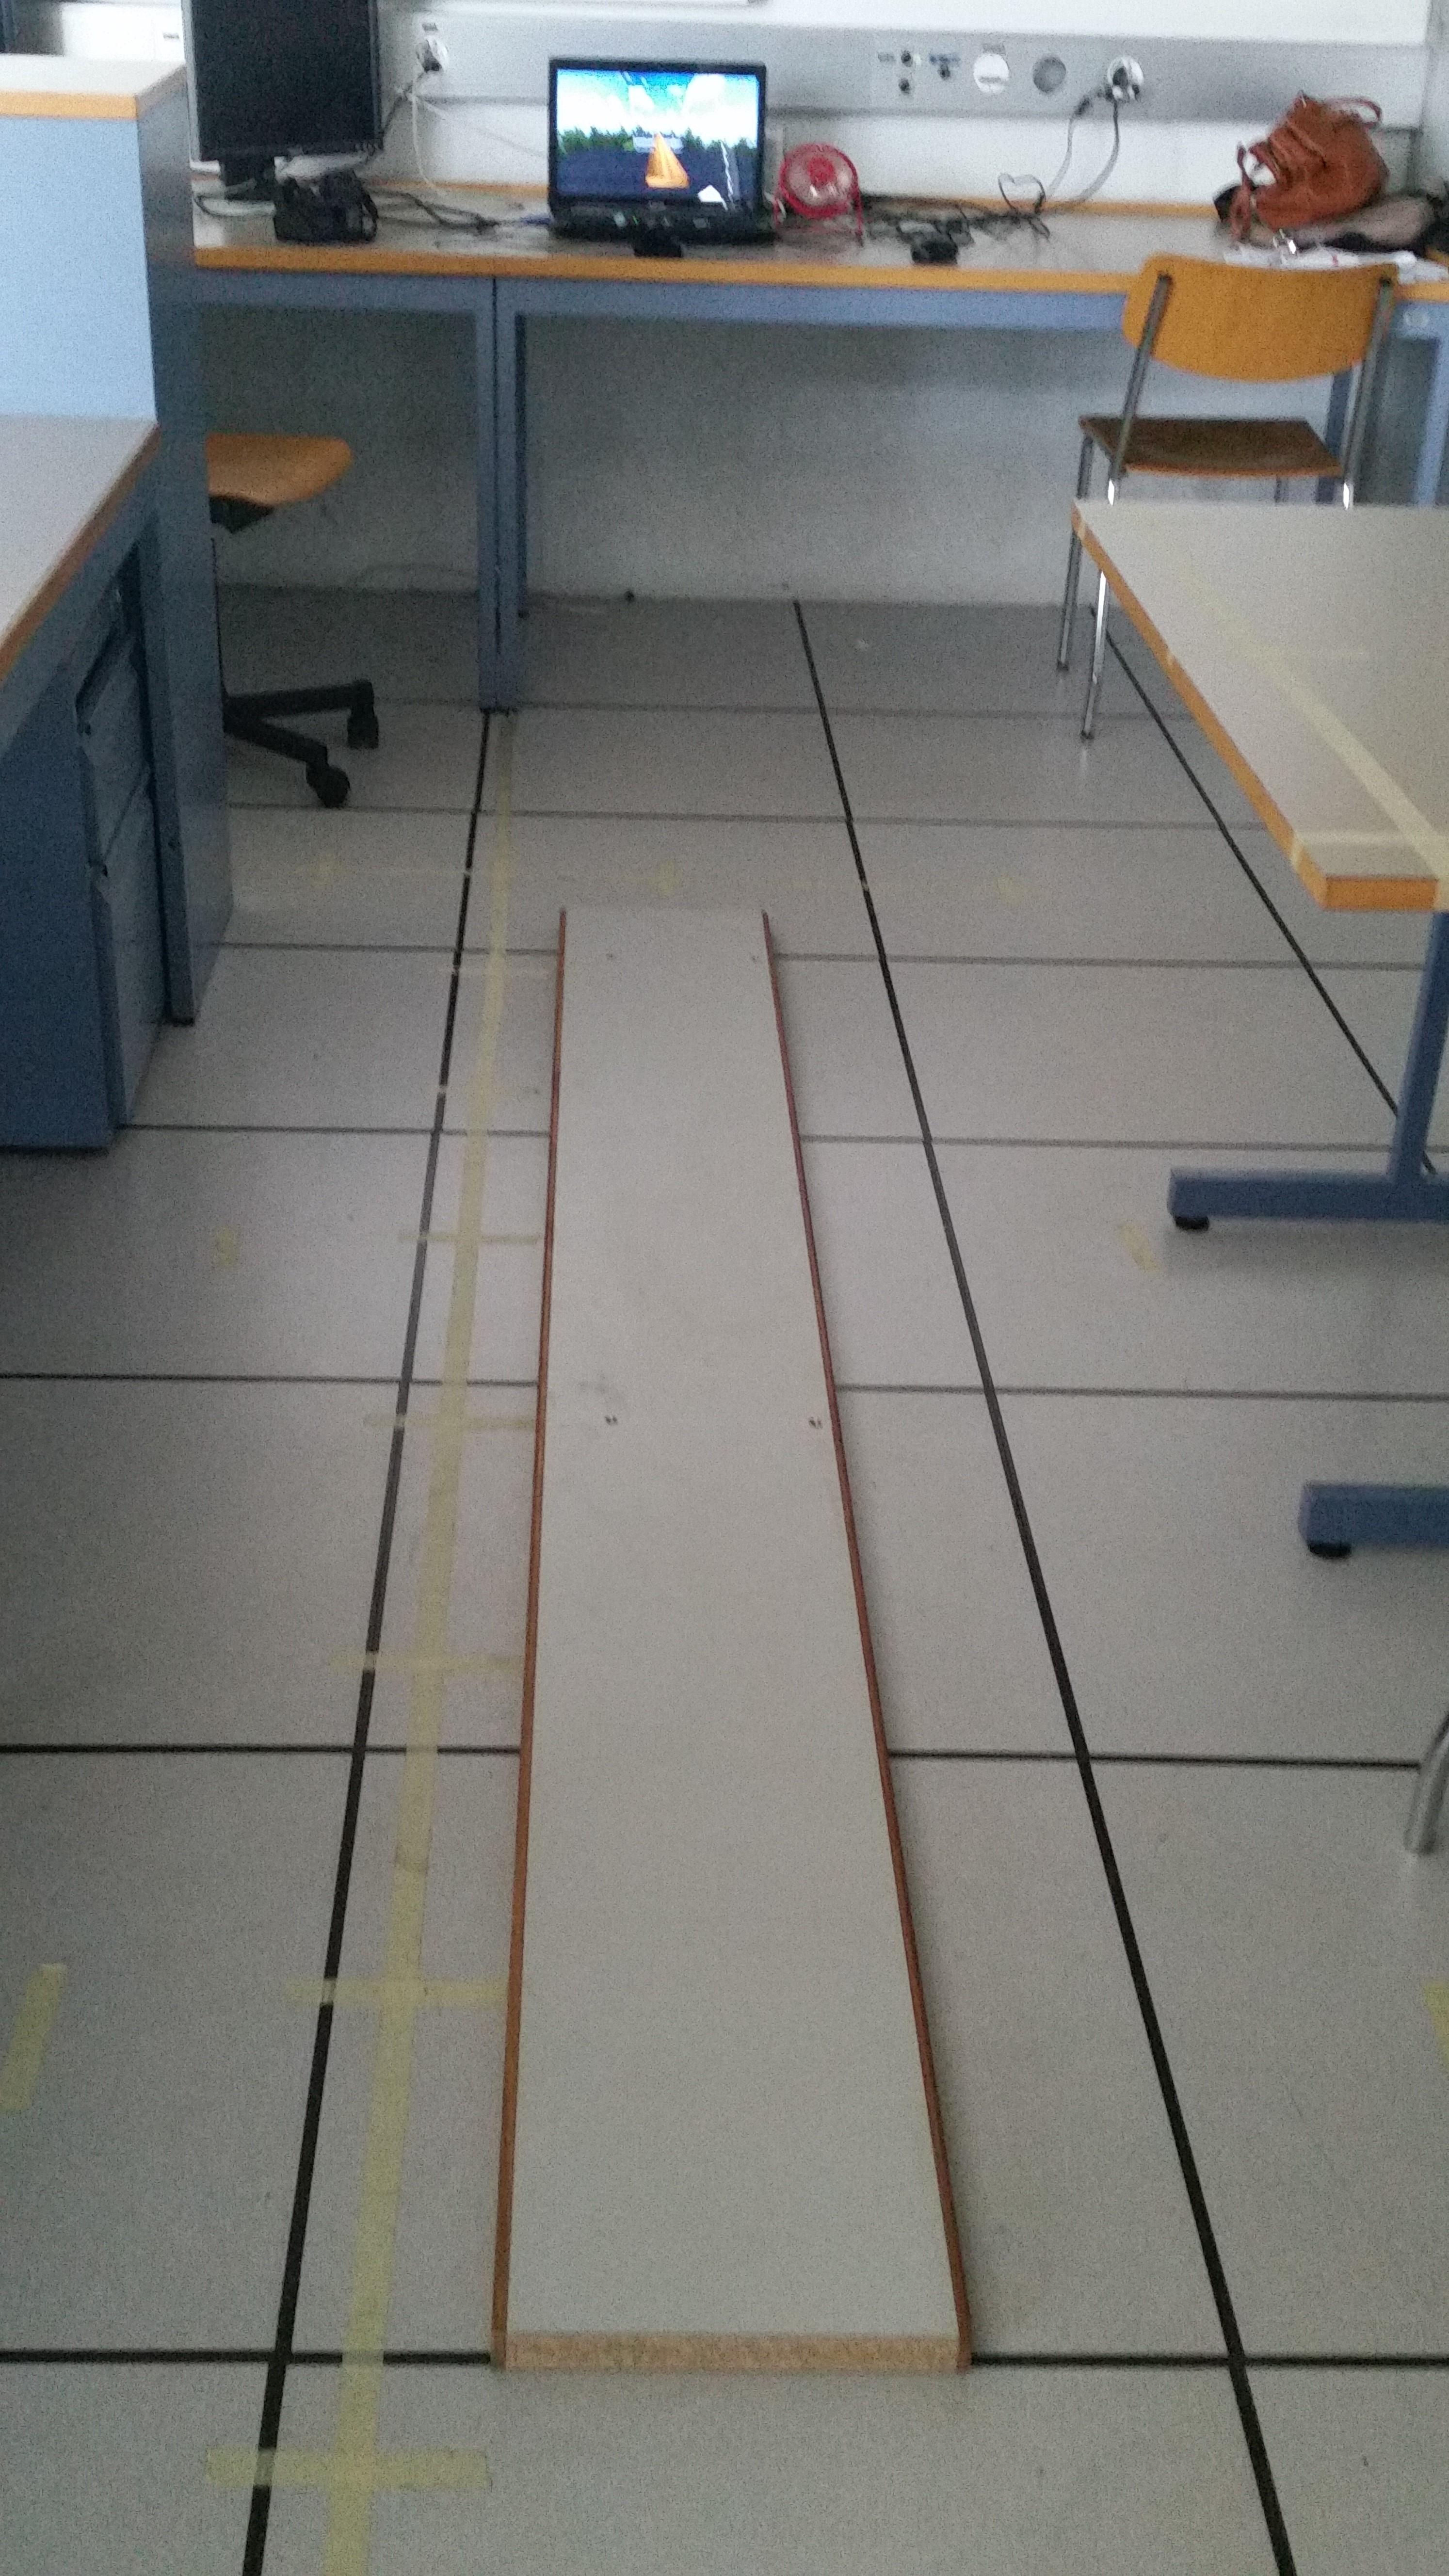
\includegraphics[scale=0.04]{vueReelle3.jpg}
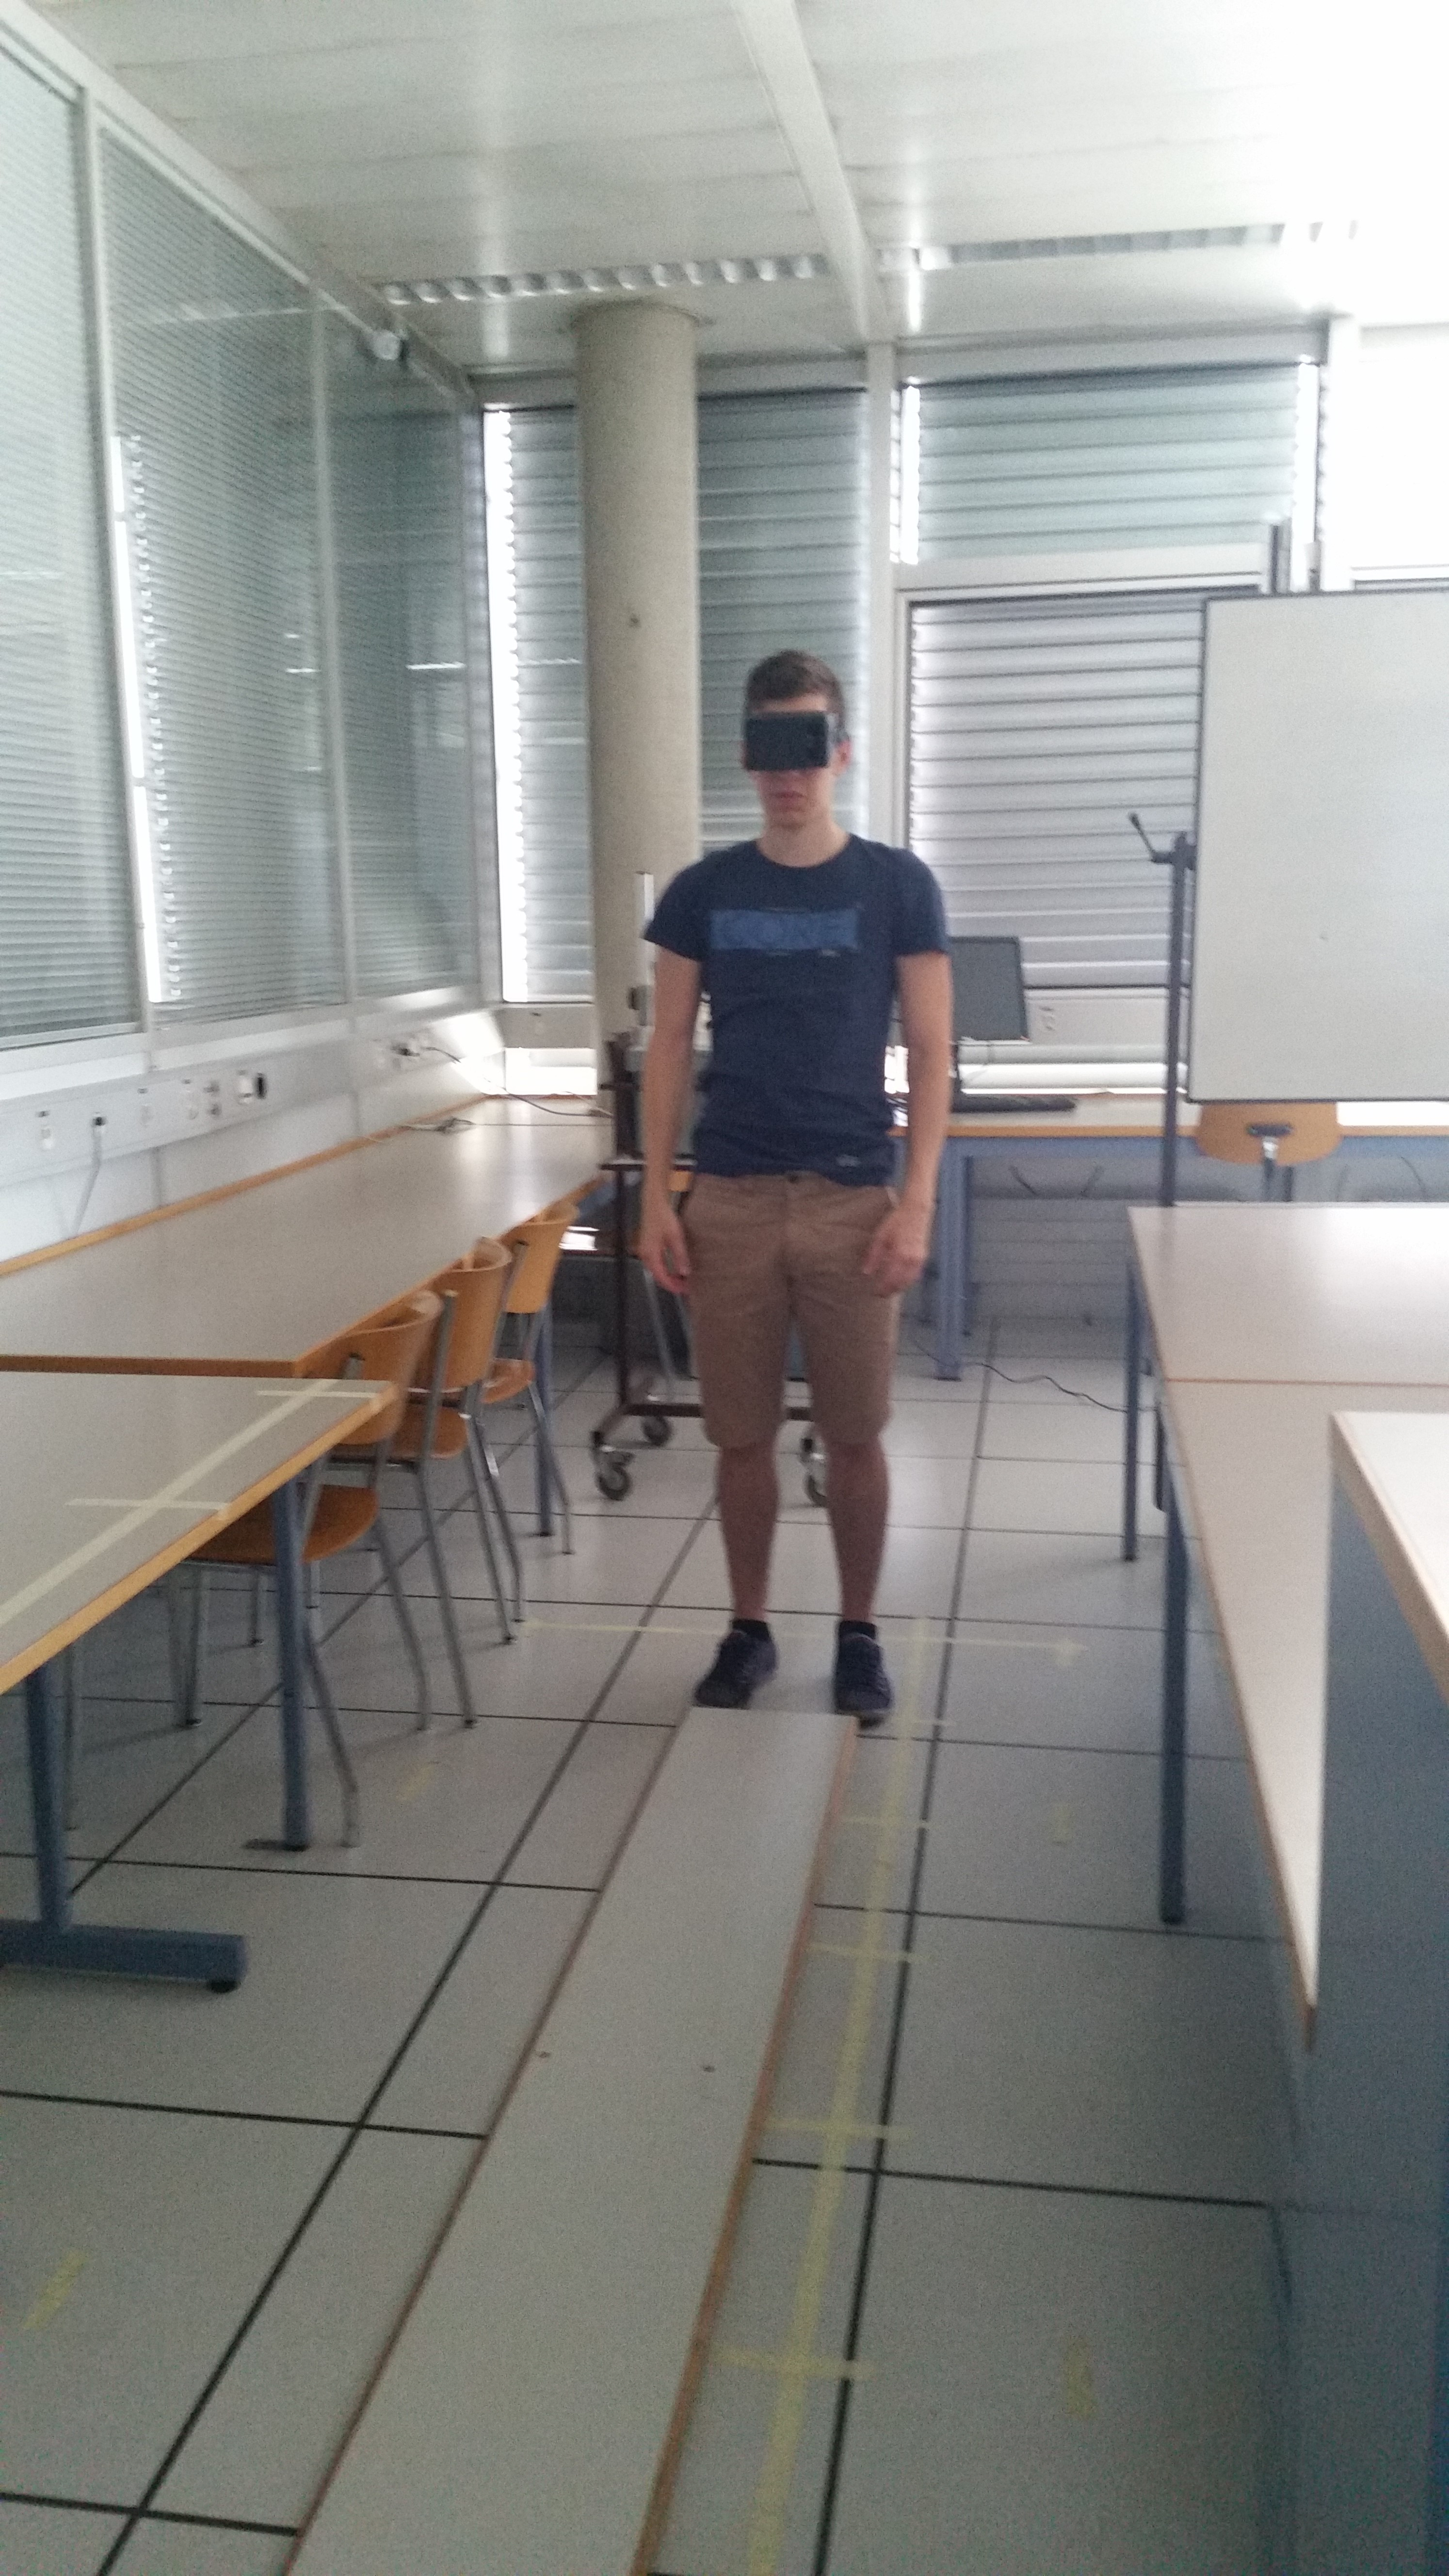
\includegraphics[scale=0.04]{vueReelle1.jpg}
\caption{\label{reelle} Illustrations de l'installation réelle mise en place}
\end{figure}

%%%%%%%%%%%%%%%%%%%%%%%%%%%%%%%%%%%%%%%%%%%%%%%%%%%%%%%%%%%%%%%%%%%%%%%%%%%%%%%%%%%%%%%%%%%%%%%%%%%%%%%%%%%%%%%%%%%%%%%%%%%

\subsection*{Effets de réalisme}  \label{realisme}
Le réalisme est très important dans ce projet. C'est pour cela que l'utilisation de quelques objets est mis en place afin de plonger la personne dans la situation la plus réaliste possible. Une planche et un effet sonore ont été ainsi ajoutés au projet.\\

\subsubsection{Planche}
Pour le ressenti de la planche sous les pieds, une planche de 2,50 mètres de distance ayant environ 5 centimètres d'épaisseur a été mise en place. Cette planche va permettre à la personne de sentir les bords de la planche quand elle s'en approche et donc d'avoir la sensation de déséquilibre et de "chute" possible. 

\subsubsection{Effet sonore environnant}
Lorsque l'utilisateur se trouve sur le toit d'un immeuble, il y a également tous les bruits environnants quotidiens, comme par exemple, les klaxons, les voitures qui passent, les gens qui parlent ou même les oiseaux. Un enregistrement des bruits sonores ambiant peut être effectué, lequel se déclencherait lorsque la personne atteint le bout de la planche. Pour cela, on envisage deux solutions possibles : \\

\begin{itemize}
\item un casque \textsf{bluetooth} qui sera connecté à l'ordinateur;
\item le \textsf{smartphone} lui-même.\\

\end{itemize}

Cette amélioration a été mise en place en utilisant le casque \textsf{bluetooth} car sur le \textsf{smartphone} il est impossible de déclencher la bande sonore sans avoir un \textsf{touch event}. \\
Ce dernier cas  sur \textsf{smartphone} n'a pas été envisagé pour une question de temps. Sinon, la bande peut être lancée lorsque la vue est mise en \textsf{fullscreen} manuellement. Le volume serait désactivé tant que  la personne n'atteint pas le bout de la planche.

\subsubsection{Sensation de vent}
Sur le toit d'un immeuble, il y a souvent du vent. C'est pour cette raison qu'un ventilateur peut être ajouté afin que l'utilisateur ressente le vent lors de l'exercice.

\subsubsection{Pulsations cardiaques}
Afin de pouvoir comparer les résultats des différentes tentatives et donc savoir si le système permet bien de vaincre la peur du vide, une montre connectée peut être utilisée. L'utilisateur devrait alors la porter lors de l'exercice. Cette montre communiquerait au serveur via le \textsf{smartphone} les informations cardiaques. Ces informations seraient stockées dans une base de données ou dans un fichier pour le suivi de l'évolution.\\
Elle permettrait également de contrôler en temps réel la personne en cas de crise ou tout autre problème physique. \\

%%%%%%%%%%%%%%%%%%%%%%%%%%%%%%%%%%%%%%%%%%%%%%%%%%%%%%%%%%%%%%%%%%%%%%%%%%%%%%%%%%%%%%%%%%%%%%%%%%%%%%%%%%%%%%%%%%%%%%%%%%%

\pagebreak
\section{Architecture}  \label{architecture}
L'architecture du projet est importante car elle permet d'avoir une application structurée et complète. L'architecture d'un projet consiste à décrire utilisant des schémas, des graphiques et des diagrammes le projet. Ici, elle contient l'organisation, la description du déroulement du projet et la description de la communication entre chaque composant présent. \\
 
Ici, l'organisation consiste à structurer en plusieurs classes ou fichiers. La séparation permet d'avoir une application mieux organisée et modulaire. Cette organisation est décrite dans la figure suivante :
\begin{figure}[H]
	\centering
   		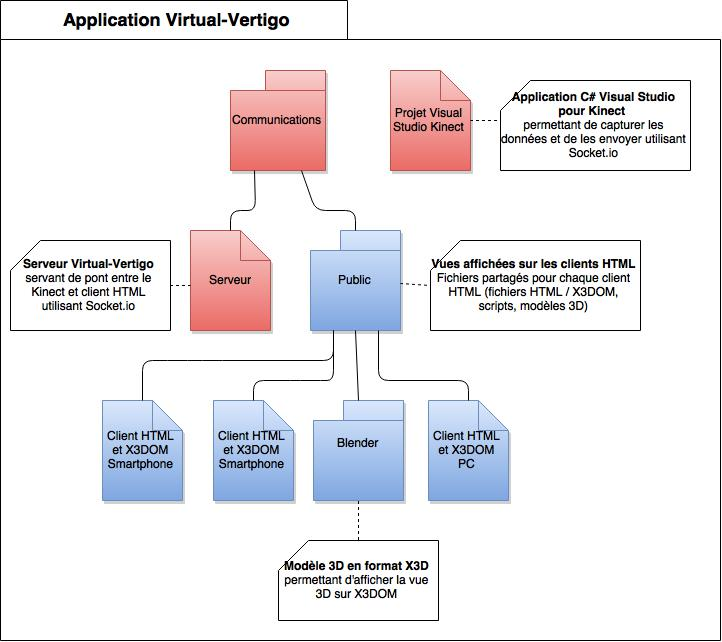
\includegraphics[scale=0.67]{Architecture.jpg}
   	\caption{\label{architecture} Architecture du projet \textit{Virtual-Vertigo}}
\end{figure}

\begin{itemize}
\item \textbf{Projet Visual Studio Kinect} : il s'agit de l'application C\# Visual Studio du \textit{Kinect}. Cette application capte les mouvements de l'utilisateur et envoie les positions aux clients via le module de communication \textit{Socket.io};
\item \textbf{Communications} : il s'agit d'un dossier contenant les fichiers privés de l'application qui gèrent la communication. Ce dossier contient aussi les fichiers nécessaires au fonctionnement du serveur;
\item \textbf{Serveur} : il s'agit du \textit{serveur Web Virtual-Vertigo}. Ce serveur correspond au pont entre le \textit{Kinect} et les clients HTML;
\item \textbf{Public} : c'est le dossier contenant les fichiers publics de l'application. Ce dossier contient les pages HTML, les scripts et les modèles 3D; 
\item \textbf{Script} : il s'agit du script modifiant la scène 3D. Ce script réceptionne les positions, crée le personnage virtuel, anime les membres de ce personnage et déplace ce personnage sur la planche;
\item \textbf{Client HTML et X3DOM Smartphone} : c'est le fichier HTML contenant la scène stéréoscopique 3D;
\item \textbf{Blender} : c'est le dossier contenant les modèles 3D ainsi que leurs textures;
\item \textbf{Client HTML et X3DOM PC} : c'est le fichier HTML contenant la scène non stéréoscopique 3D affichée sur un écran standard.\\ \linebreak
 
\end{itemize} 

A noter que les éléments en rouge sont des éléments privés que seul la personne s'occupant du serveur peut avoir accès. Les éléments en bleu contiennent les éléments publiques. C'est-à-dire, les clients HTML (\textsf{smartphone} et PC), les scripts JavaScript interagissant avec la vue et les modèles 3D. Plus de détails sur ces composants logiciels sont donnés au chapitre~\ref{implementation}.\\

 
La description du déroulement du projet consiste, via un diagramme ou un schéma, à montrer la vie du projet. C'est à dire, décrire ce qu'il se passe entre chaque événement et comment le changement d'événement s'effectue. Le déroulement du projet est illustré par le diagramme de séquence~\ref{sequence} :
\begin{figure}[H]
	\centering
   		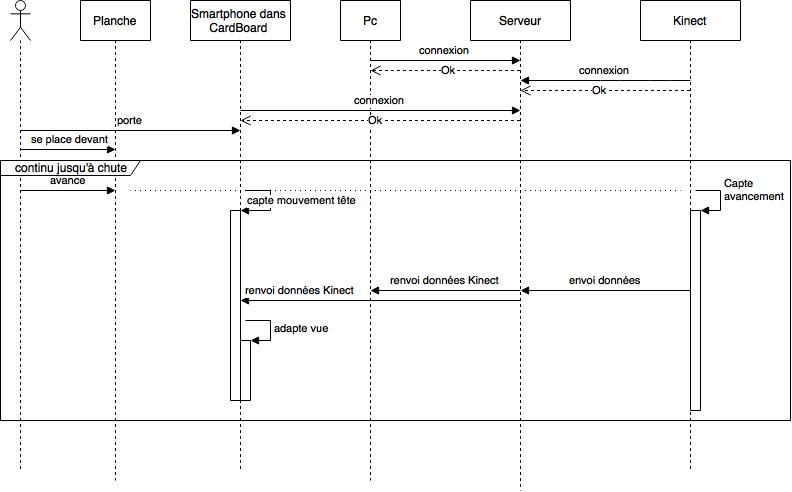
\includegraphics[scale=0.6]{VertigoSequence.jpg}
   	\caption{\label{sequence} Diagramme de séquence du projet \textit{Virtual-Vertigo}}
\end{figure}

Ce diagramme montre deux phases : l'une d'initialisation, et l'autre de simulation. L'initialisation correspond au lancement du serveur, puis la connexion du \textsf{smartphone} et du \textit{Kinect} à ce serveur. La phase de simulation commence quand l'utilisateur se place devant la planche. Une fois la simulation démarrée, les opérations suivantes sont effectuées en boucle : 

\begin{itemize}
\item le Kinect capte les mouvements de la personne;
\item le Kinect transmet les positions au serveur;
\item le serveur retransmet ces positions aux clients HTML connectés;
\item Les clients HTML adaptent leurs vues.\\

\end{itemize}
Cette boucle s'exécute toutes les secondes et s'arrête quand la personne "chute" ou quand elle arrive au bout de la planche.\\

Le déroulement du projet peut également être détaillé en se basant sur les différents états durant la simulation. Le diagramme~\ref{activiteDiag} montre les états des composants du projet et l'action qui les fait changer d'état.
\begin{figure}[H]
	\centering
   		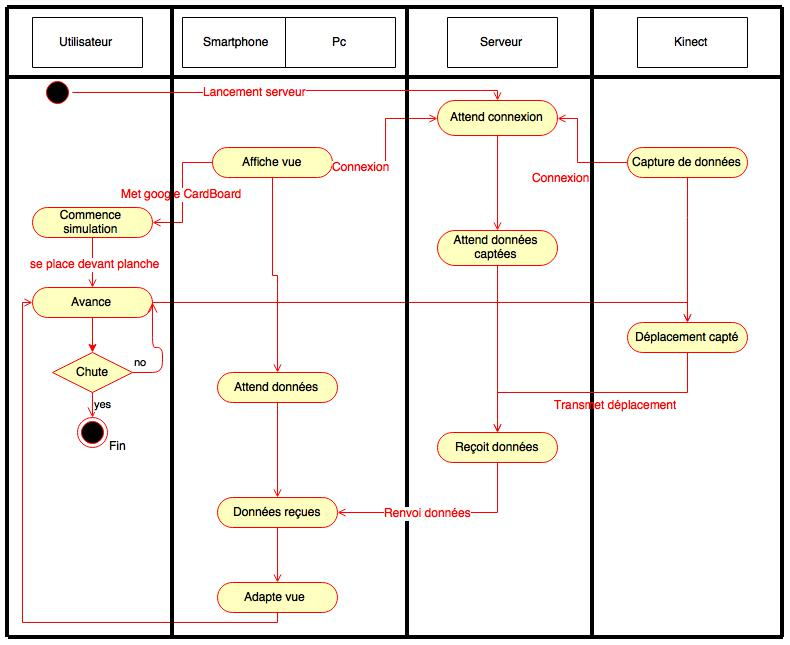
\includegraphics[scale=0.6]{VertigoActivite.jpg}
   	\caption{\label{activiteDiag} Diagramme d'activité du projet \textit{Virtual-Vertigo}}
\end{figure} 
L'application commence par le lancement du serveur qui se met en attente d'une connexion d'un client. Lorsque le \textit{Kinect} et les clients HTML se connectent, le serveur attend de recevoir les positions captées par le \textit{Kinect} pour ensuite les retransmettre aux clients HTML. Lors de la réception des positions, les clients adaptent la vue virtuelle. En parallèle, l'utilisateur effectue sa simulation de réalité virtuelle.





\chapter{Composants, technologies et outils}  \label{outils}
Ce chapitre décrit tous les composants, technologies et outils nécessaires à la réalisation du projet \textit{Virtual-Vertigo}. Pour chaque section, un exemple d'utilisation général a été inclus. 
%%%%%%%%%%%%%%%%%%%%%%%%%%%%%%%%%%%%%%%%%%%%%%%%%%%%%%%%%%%%%%%%%%%%%%%%%%%%%%%%%%%%%%%%%%%%%%%%%%%%%%%%%%%%%%%%%%%%%%%%%%%

\section{Google CardBoard} \label{cardboard}

Les \textit{Google CardBoard} sont des casques de réalité virtuelle en carton équipé de deux lentilles et dans lesquels peut venir se loger un \textsf{smartphone}. Elles se construisent à la maison avec très peu de matériel et sont accessibles à tout le monde à un prix très bas. Google permet ainsi via ses lunettes de pouvoir utiliser des applications de réalité virtuelle 3D sans avoir à mettre une somme d'argent trop importante.

\subsection*{Version 1}
\begin{figure}[h]
	\centering
		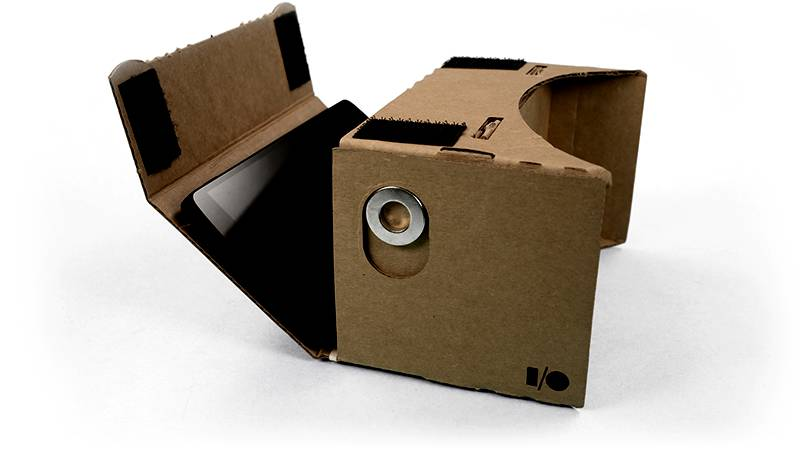
\includegraphics[scale=0.15]{CardBoard1.jpg}
		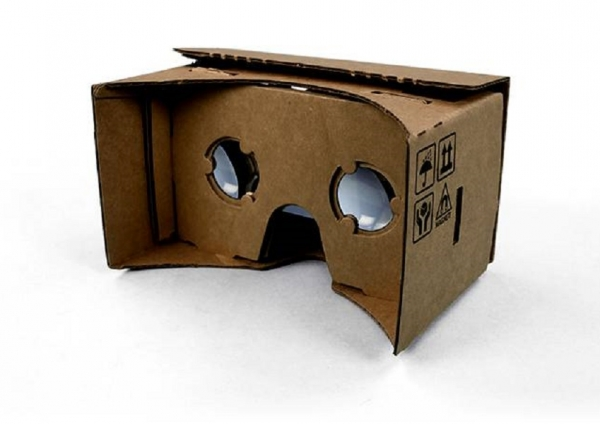
\includegraphics[scale=0.15]{CardBoard1-2.jpg}
	\caption{\label{CardBoard1} Illustrations des \textit{Google CardBoard version 1}}
\end{figure}

La première version des \textit{Google CardBoard} a été introduite en 2014.

\subsubsection{Matériel pour le montage}
Pour la construction, il ne faut pas grand chose :
\begin{itemize}
\item du carton pas trop épais (1-2 millimètres)
\item deux lentilles biconvexes
\item un tag NFC
\item un aimant céramique
\item un aimant néodyme
\item du velcro \\

\end{itemize}

A noter que les aimants servent à interagir avec le \textsf{smartphone} pour actionner les boutons. \\

Les patrons de conception et les instructions de montage sont mis à disposition sur le site des \textit{Google CardBoard} \cite{CardBoard}. Il suffit alors de les imprimer, les coller sur le carton, découper et assembler tout les composants pour obtenir des \textit{Google CardBoard}. Il est également possible d'acheter des \textit{Google CardBoard} pré-fabriquées.\\

Dans le cadre du Projet \textit{Virtual-Vertigo}, les \textit{Google CardBoard} utilisées ont complètement été construites manuellement. Cependant, seules les lentilles biconvexes ont servi. En effet, l'aimant et le patch NFC n'ont pas été utilisé pour \textit{Virtual-Vertigo}.\\

A noter qu'un tutoriel contenant les instructions pour le montage des \textit{Google CardBoard} est disponible en annexe.

\subsection*{Version 2} 
\begin{figure}[h]
	\centering
		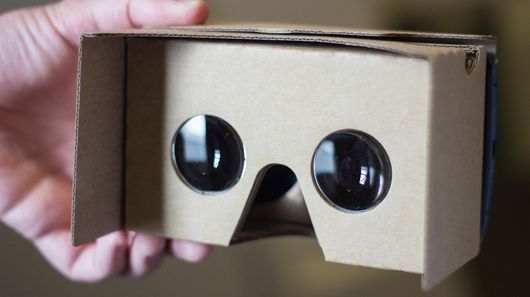
\includegraphics[scale=0.25]{CardBoard2.jpg}
		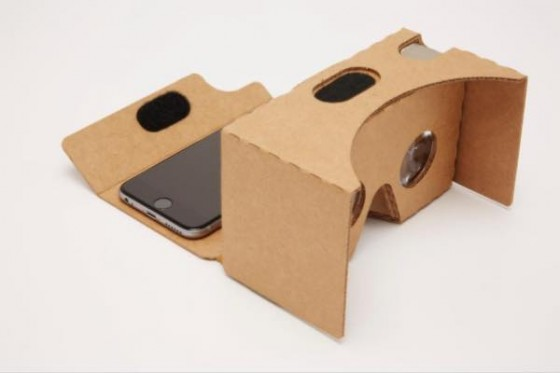
\includegraphics[scale=0.2]{CardBoard2-1.jpg}
	\caption{\label{CardBoard2} Illustrations des Google CardBoard version 2}
\end{figure}
La nouvelle version des Google CardBoard est sortie en juin 2015

\subsubsection{Nouveautés}
\begin{itemize}
	\item Cette version est capable de contenir un \textsf{smartphone} jusqu'à 6 pouces.
	\item Les aimants étant pas fiable sur la version 1 ont été remplacés par un bouton physique interagissant directement avec le \textsf{smartphone}.
	\item Google a implémenté un SDK qui supporte les \textsf{iPhones} et les \textsf{Android}.
	\item Le montage est plus simple.
\end{itemize}

\subsubsection{Matériel pour le montage}
Google n'a pas encore transmis les patrons de conception ni la liste de matériel pour construire cette nouvelle version.

\pagebreak
\subsection*{Vision stéréoscopique sur le smartphone} \label{vision}
La stéréoscopie est une technique mise en oeuvre pour reproduire une perception de 3D à partir de deux images. Elle se base sur le fait que la perception humaine de la 3D se forme dans le cerveau lorsqu'il reconstitue une seule image à partir de la perception de deux images provenant de chaque oeil. \\

La stéréoscopie pour les \textit{Google CardBoard} s'effectue sur le \textsf{smartphone}. La vue affichée sur le \textsf{smartphone} doit avoir une vue pour chaque oeil. Puis c'est par l'intermédiaire des lentilles que ses images planes seront perçues comme des images 3D.

\begin{figure}[H]
\centering 
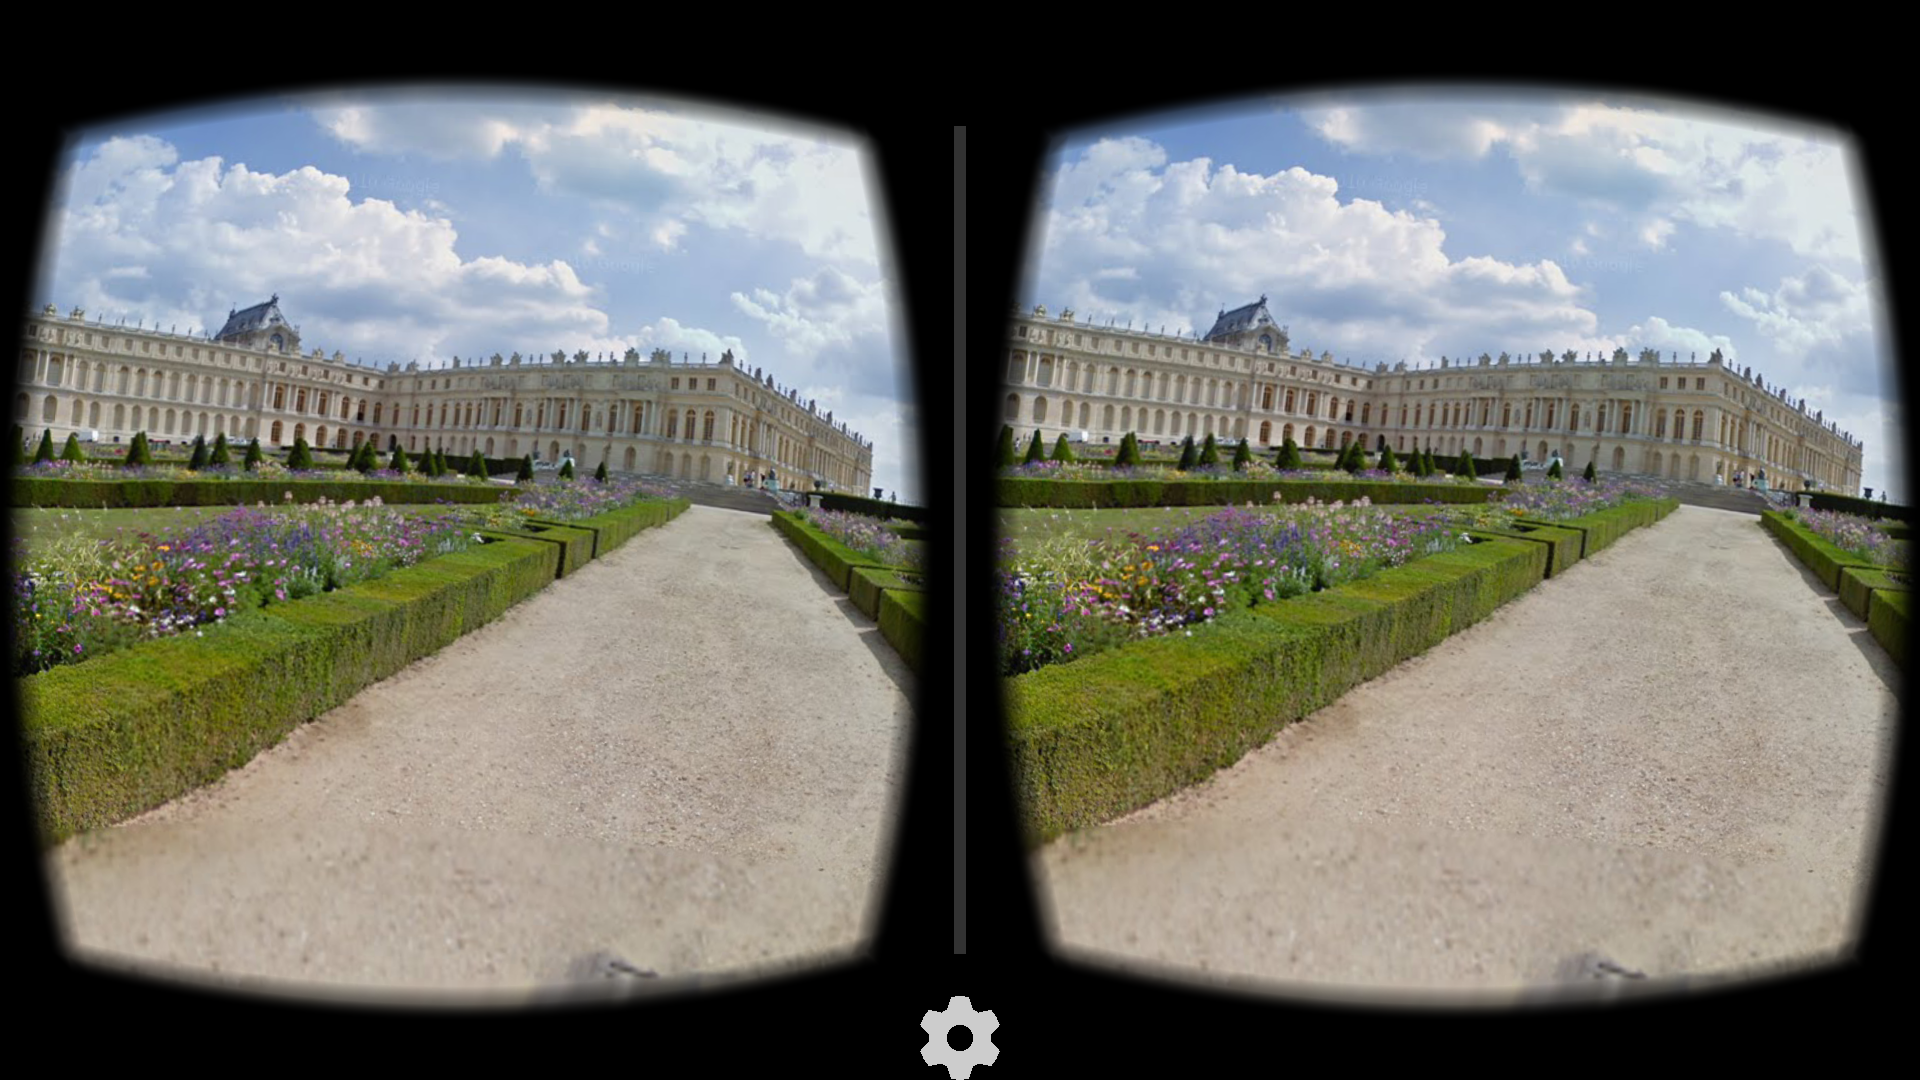
\includegraphics[scale=0.1]{stereoscopie.png}
\caption{\label{sterescopie} Stéréoscopie sur smartphone pour \textit{Google CardBoard}}
\end{figure}

Pour plus d'informations sur la stéréoscopie, voir \cite{stereoscopie}.

\subsection*{Applications sur Google CardBoard}  \label{applications}
La vue sur le \textsf{smartphone} doit absolument être stéréoscopique afin que les lentilles donnent un effet de 3D. Ainsi, en plaçant le \textsf{smartphone} dans les \textit{Google CardBoard} avec une application pour \textsf{CardBoard} lancée, l'immersion dans le monde virtuel est immédiate. \\

Une application utilisant les \textit{Google CardBoard} doit être stéréoscopique et peut par exemple être implémentée en deux langages différents : 
\begin{itemize}
\item comme une application \textsf{Android} en Java : cela implique que tout est stocké et exécuté sur le \textsf{smartphone};
\item comme une application Web via un Framework 3D : cela implique que le \textsf{smartphone} charge seulement une page Web.
\end{itemize}

\subsubsection*{Applications disponibles}  \label{dispo}
Plusieurs applications sont disponible pour les \textit{Google CardBoard} implémentée sur \textsf{Android} ou le Web. Ci-dessous, la description d'une application \textsf{Android} suivi de la description d'une application Web pour les \textit{Google CardBoard}.\\
L'\textsf{application Android CardBoard} disponible sur le play store permet de tester plusieurs démonstrations sur les Google CardBoard. Pour vous procurer l'application \textsf{CardBoard}, voir \cite{androidCardboard}. Ci-dessous la liste des démonstrations que l'application propose : 
\pagebreak
\begin{itemize}
\item \textbf{Earth : } aller où vous voulez avec \textsf{Google Earth};
\item \textbf{Tour Guide : } visiter Versailles avec un guide;
\item \textbf{My Videos : } regarder vos vidéos sur un grand écran;
\item \textbf{Exhibit : } examiner un artefact culturel sous différents angles;
\item \textbf{Photo Sphere : } regarder vos photos sphère;
\item \textbf{Windy Day : } suivre une histoire dans une courte scène interactive de \textsf{Google Spotlight Stories}, votre cinéma de poche (pour plus d'informations sur \textsf{Google Spotlight Stories}, voir \cite{spotlight}).\\

\end{itemize}
L'\textsf{application ClassroomVR} disponible sur internet utilise le \textit{Framework X3DOM} (voir section~\ref{x3dom}). Cette application met en scène une salle de classe stéréoscopique 3D. Ci-dessous une illustration de cette application : 

\begin{figure}[H]
\centering
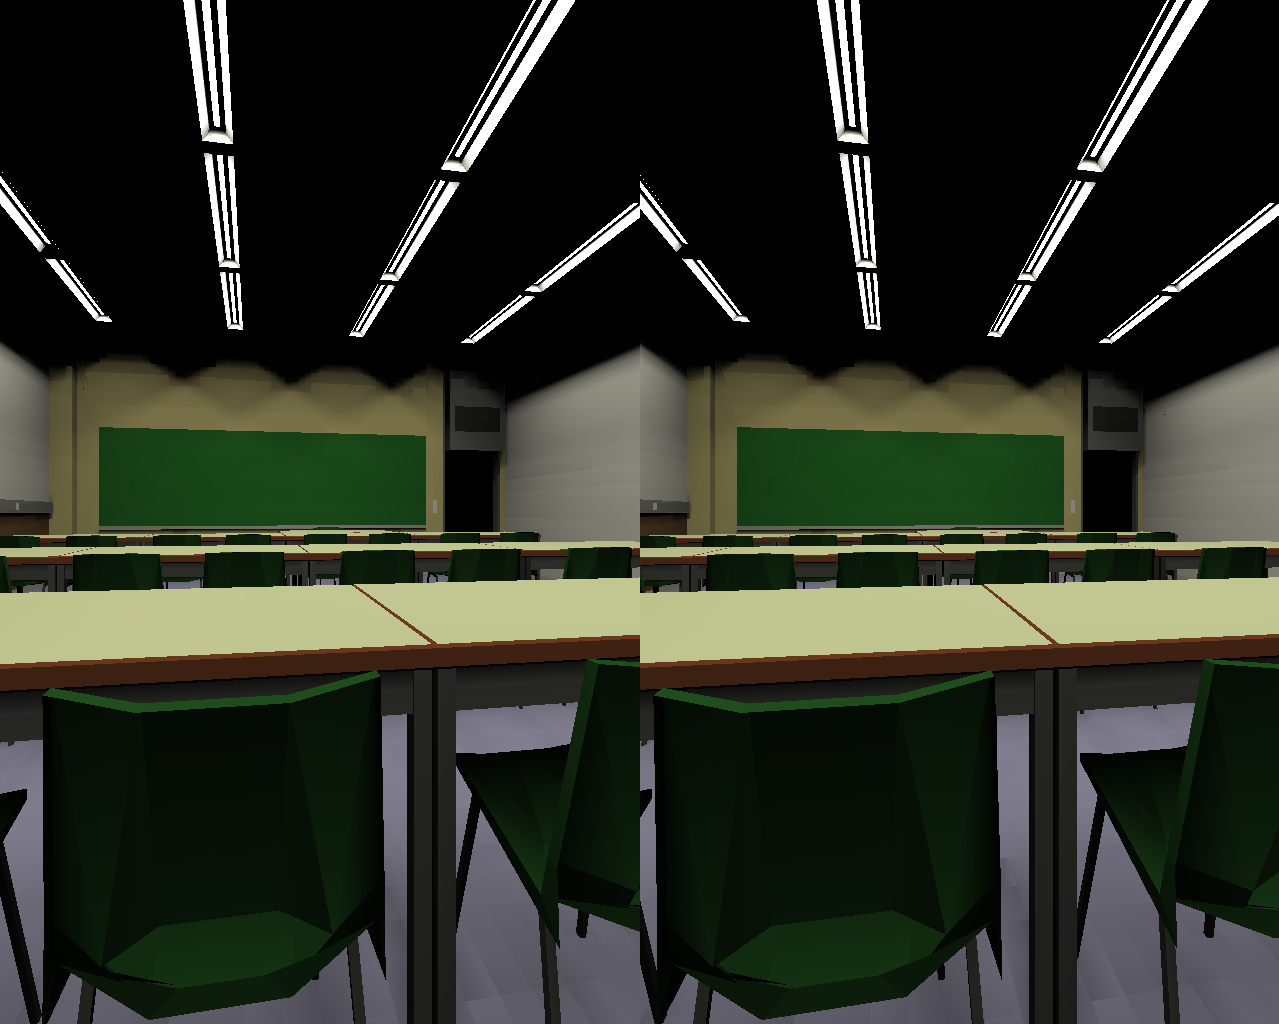
\includegraphics[scale=0.4]{classroom.png}
\caption{\label{classroom} Illustration de l'\textsf{application ClassroomVR}}
\end{figure}
La scène~\ref{classroom} met en scène une salle de classe contenant des tables, des chaises et un tableau noir. Lorsque cette vue est visualisée via les lentilles des \textit{Google CardBoard}, la personne est plongée dans cette salle et peut l'observer depuis un point fixe.


%%%%%%%%%%%%%%%%%%%%%%%%%%%%%%%%%%%%%%%%%%%%%%%%%%%%%%%%%%%%%%%%%%%%%%%%%%%%%%%%%%%%%%%%%%%%%%%%%%%%%%%%%%%%%%%%%%%%%%%%%%%
 
\pagebreak 
\section{Kinect version 1}  \label{kinect}
Le \textit{Kinect} est un périphérique initialement destiné à la \textsf{console de jeux Xbox 360}. Il permet à l'utilisateur d'interagir en utilisant son corps plutôt qu'une manette. Depuis quelques années, Microsoft a mis à disposition un SDK permettant d'utiliser le \textit{Kinect} sur un ordinateur Windows. Cependant, le Kinect nécessite des caractéristiques hardware spécifiques (pour plus d'informations sur les caractéristiques du\textit{ Kinect v1}, voir~\cite{PrerequisKinectv1}).\\

Le \textit{Kinect} a été choisi pour capter et reporter les mouvements et le déplacement de la personne. Ainsi grâce au \textit{Kinect}, la personne peut voir ses mains ou ses pieds (en simplifié) lorsqu'il avance sur la planche. Le \textit{Kinect version 1} a été choisi en particulier car l'école disposait déjà d'un tel appareil et également parce qu'il convenait amplement aux besoins de \textit{Virtual-Vertigo}.\\

A noter qu'un tutoriel contenant les instructions pour l'installation et l'utilisation du \textit{Kinect v1} est disponible en annexe.

\subsection{Composants et caractéristiques}  \label{composant}
Cette section contient une description succincte des composants et caractéristiques du \textit{Kinect v1}.
\begin{figure}[h]
	\centering
		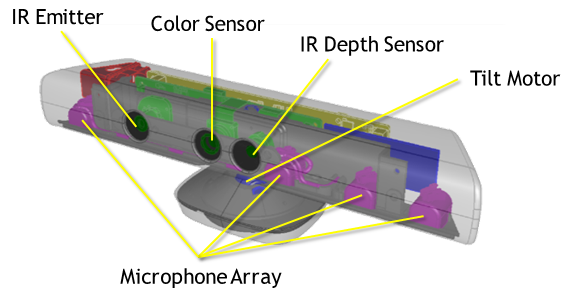
\includegraphics[scale=0.5]{SpecKinect.png}
	\caption{\label{SpecKinect} Structure du \textit{Kinect version 1}}
\end{figure}

\begin{itemize}
	\item \textbf{Color Sensor : } caméra RGB
	\item \textbf{IR Emitter : } émet des infrarouges pour le Depth Sensor
	\item \textbf{IR Depth Sensor : } lit les infrarouges retournés au Kinect, puis les convertis en information de 	profondeur mesurant la distance entre l'objet et le Kinect
	\item \textbf{Tilt Motor : } permet de changer et de déterminer l'orientation du \textit{Kinect v1} sur un axe 3D
	\item \textbf{Microphone Array : } 4 microphones qui permettent de capturer le son\\
\end{itemize}

\begin{center}
	\begin{tabular}{| l | c |}
	\hline
		\textbf{Max Distance} & ~4.5 m \\ \hline
		\textbf{Min Distance} & 0.8 m (normal mode) and 0.4 m (near mode)\\ \hline
		\textbf{Horizontal Field Of View} & 57 degrees \\ \hline
		\textbf{Vertical Field Of View} & 43 degrees \\ \hline
		\textbf{Frame Rate} & 30 fps \\ \hline
		\textbf{Skeleton Joints Defined} & 20 \\ \hline
		\textbf{Full Skeleton Tracked} & 2 \\ \hline
		\textbf{Audio Format} & 16 kHz (24 bit mono PCM) \\ \hline
		\textbf{Vertical Tilt Range} & +- 27 degrees \\
		\hline
	\end{tabular}
	\captionof{table}{\label{spec} Tableau illustrant les caractéristiques du \textit{Kinect v1}}
\end{center}


\subsubsection{Comparaison v1 et v2}

\begin{figure}[h]
	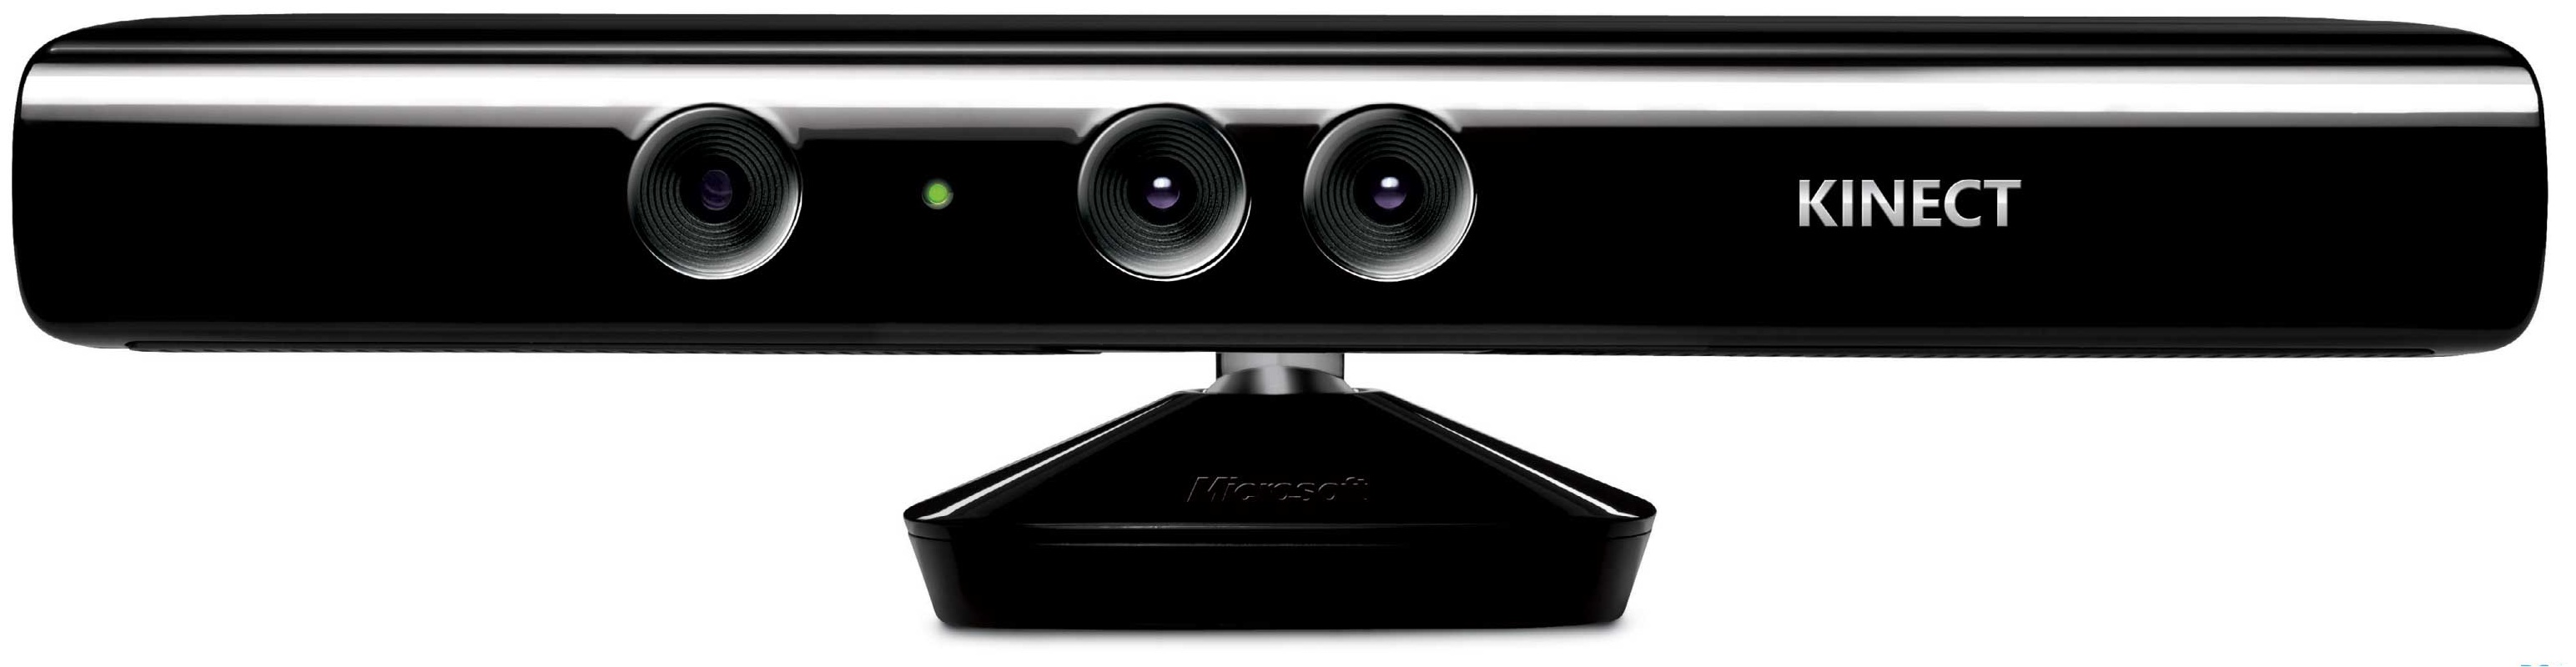
\includegraphics[scale=0.1]{Kinectv1.jpeg}
	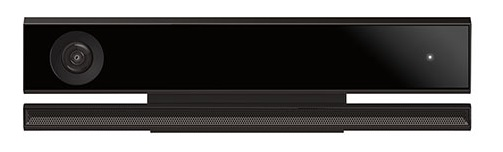
\includegraphics[scale=0.5]{Kinectv2.jpg}
	\caption{\label{Kinectv1v2} Kinect v1 vs Kinect v2}
\end{figure}
\begin{itemize}
	\item la plus grande différence entre les 2 versions est la résolution.\\
	 La résolution couleur est plus de 3 fois plus élevée et la résolution de profondeur est quasiment 2 fois plus élevée.
	\item les champs de vue horizontal et vertical ont également augmenté. 
	\item 25 articulations sont captées par le \textit{Kinect v2} contre 20 pour le \textit{Kinect v1}.
	\item le principal défaut du \textit{Kinect v2} est que les caractéristiques hardware sont plus exigeantes.
	\item le nombre de fps (Frame par secondes) n'a pas changé entre les 2 versions. 
\end{itemize}

\subsection{Capture des données}
Le \textit{Kinect} permet de capter différents types de données d'une personne de plusieurs manières. Les différentes captures se font en utilisant les capteurs du \textit{Kinect}.\\

Le \textit{Kinect} permet de capturer les données d'une personne dans 2 positions différentes : \textsf{default}, la personne est debout, et \textsf{seated}, la personne est assise. Les informations ci-dessous peuvent être capturés dans les deux positions. 
\pagebreak
\subsubsection{Angle de vue}
Le \textit{Kinect} capte les informations sur un rayon de 43 degrés à la verticale et de 57 degrés à l'horizontale. L'angle de vue du \textit{Kinect} se traduit comme un cône, le \textit{Kinect} étant la partie la plus étroite du cône.\\

Ci-dessous une illustration des angles de vue du \textit{Kinect}.
\begin{figure}[H]
	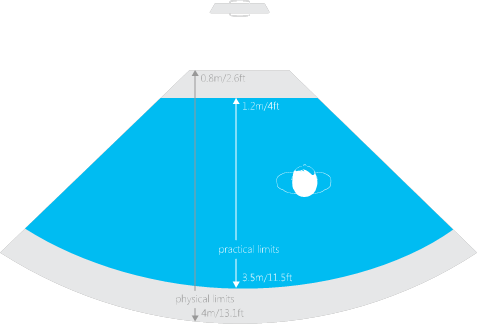
\includegraphics[scale=0.5]{fieldviewHorizontal.png}
	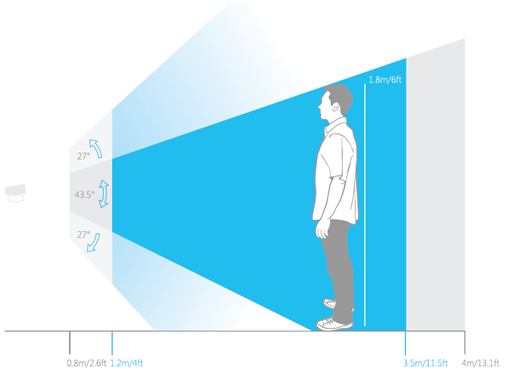
\includegraphics[scale=0.5]{fieldviewVertical.png}
	\caption{\label{AngleVue} Angles de vue du \textit{Kinect} horizontal et vertical}
\end{figure}

\subsubsection{Color Stream}
Le \textsf{Color Stream} sert de caméra RGB au \textit{Kinect}. Il retransmet les informations que le \textsf{Color Sensor} capte. Il permet donc d'afficher et de modifier la vue en temps réel. \\

Il permet d'utiliser plusieurs formats différents :  
\begin{itemize}
\item Raw YUV, résolution de $640\times 480$ à 15 fps 
\item RGB, résolution de $1280\times 960$ à 12 fps
\item RGB, résolution de $640\times 480$ à 30 fps
\item YUV, résolution de $640\times 480$ à 15 fps
\item Infrared de type MONO16, résolution de $640\times 480$ à 30 fps permet de capter en cas de lumière faible
\item RawBayer de type MONO8, résolution de $1280\times 960$ à 12 fps ou  de $640\times 480$ à 30 fps pour utiliser son propre algorithme de reconstruction d'image
\end{itemize}
Le \textsf{Color Sensor} n'est pas utilisé dans ce projet.

\subsubsection{Depth Stream}
Le \textsf{Depth Stream} sert à capter les informations en utilisant la profondeur détectée par les infrarouges. Il permet donc d'afficher et de modifier le vue en profondeur avec des nuances de gris.
Il capte la profondeur en deux modes : \textsf{default}, de 0.6 à 4m, et \textsf{near}, de 0.4 à 3m. \\
Il permet également de le faire à 30 fps en différentes dimensions : $640\times 480$, $320\times 240$ et $80\times 60$.\\ 
Le \textsf{Depth Stream} n'est pas utilisé dans ce projet.

\pagebreak
\subsubsection{Skeletal Stream}
Le \textsf{Skeletal Stream} retourne les positions du squelette ainsi que la position, en 3 dimensions, de chacune des 20 articulations de référence sur le squelette en mètres (voir section~\ref{articulation}). \\
Il faut savoir que l'origine est le \textit{Kinect}, que les axes x et y sont les offset du centre de vision du \textit{Kinect} et que l'axe z est la distance entre le \textit{Kinect} et l'objet.\\

\begin{figure}[H]
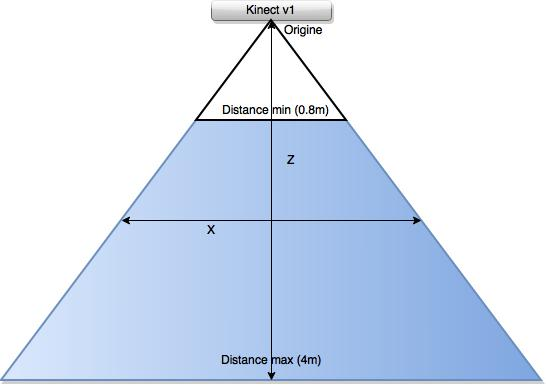
\includegraphics[scale=0.4]{SkeletonX.jpg}
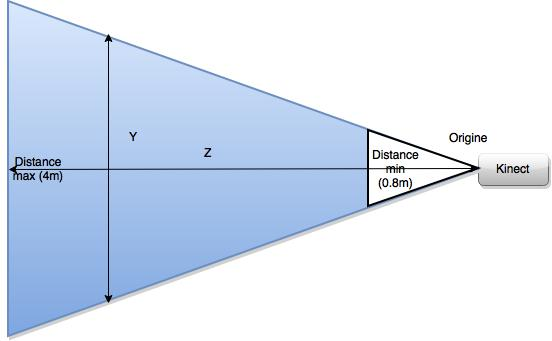
\includegraphics[scale=0.4]{SkeletonY.jpg}
\caption{\label{positions} Illustration des axes par rapport au \textit{Kinect}}
\end{figure}
Le figure~\ref{positions} illustre comment sont placé les axes x, y et z en fonction du \textit{Kinect}. La partie verte sur chaque figure correspond à la zone que le \textit{Kinect} capte.


\subsection{Articulations du squelette et leurs orientations} \label{articulation} 
\begin{figure}[h]
	\centering
		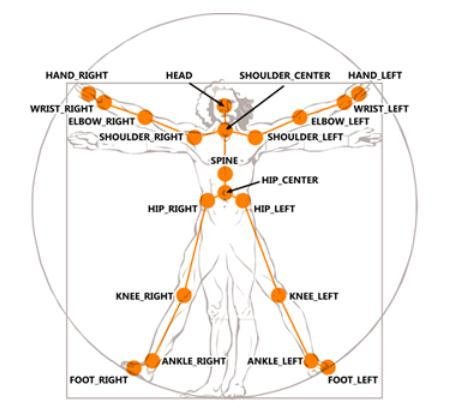
\includegraphics[scale=0.47]{squelette.jpg}
	\caption{\label{Joints} Articulations du squelette captés par le Kinect}
\end{figure}
Les 20 articulations que le \textit{Kinect v1} détecte se trouvent sur l'illustration~\ref{Joints}. A chacune de ces articulations correspond un identifiant qui permet ensuite de retrouver le nom de l'articulation détectée. Le tableau~\ref{valeurs} ci-dessous donne ces valeurs.
\begin{center}
	\begin{tabular}{| c | c | c |}
	\hline
		\textbf{Identifiant} & \textbf{Articulation} & \textbf{Nom sur squelette} \\ \hline
		0 & base of the spine & hipcenter \\ \hline
		1 & middle of the spine & spine \\ \hline
		2 & neck & shouldercenter \\ \hline
		3 & head & head \\ \hline
		4 & left shoulder & shoulderleft \\ \hline
		5 & left elbow & elbowleft \\ \hline
		6 & left wrist & wristleft \\ \hline
		7 & left hand & handleft \\ \hline
		8 & right shoulder & shoulderleft \\ \hline
		9 & right elbow & elbowright \\ \hline
		10 & right wrist & wristright \\ \hline
		11 & right hand & handright \\ \hline
		12 & left hip & hipleft \\ \hline
		13 & left knee & kneeleft \\ \hline
		14 & left ankle & ankleleft \\ \hline
		15 & left foot & footleft \\ \hline
		16 & right hip & hipright \\ \hline
		17 & right knee & kneeright \\ \hline
		18 & right ankle & ankleright \\ \hline
		19 & right foot & footright \\ \hline
		20 & spine at the shoulder & n'est pas détecté \\ \hline
		21 & tip of the left hand & n'est pas détecté \\ \hline
		22 & left thumb & n'est pas détecté \\ \hline
		23 & tip of the right hand & n'est pas détecté \\ \hline
		24 & right thumb & n'est pas détecté \\
		\hline
	\end{tabular}
\captionof{table}{\label{valeurs} Tableau illustrant les valeurs de chaque articulation}
\end{center}

Le \textit{Kinect v1} capture également l'orientation des articulations du squelette. Connaître l'orientation des articulations du squelette permet d'effectuer une plus précise animation d'un avatar. Le \textit{Kinect v1} peut capter l'orientation de deux manières : la rotation hiérarchique, basé sur les membres reliés, et l'orientation absolue, utilisant les coordonnées de la caméra. \\

Les deux images ci-dessous illustrent comment le \textit{Kinect v1} capture l'orientation des articulations du squelette :
\begin{figure}[H]
\centering
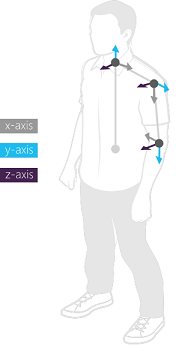
\includegraphics[scale=0.6]{hierachical.png}
\caption{\label{hierachical} Illustration de la rotation hiérachique}
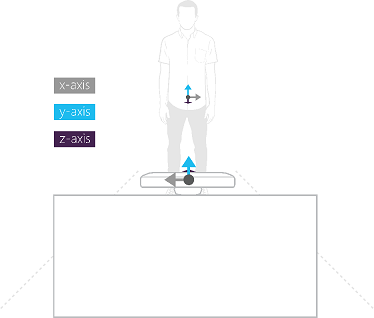
\includegraphics[scale=0.6]{absolute.png}
\caption{\label{absolute} Illustration de l'orientation absolue}
\end{figure}
Pour plus d'informations sur les orientations des articulations, voir \cite{jointOrientation}.
Ces données d'orientations peuvent être retournées sous forme de quaternions ou de matrices de rotations. Ci-dessous une illustration des deux formes : 
\begin{equation}
q = r + x\textbf{j}  + y\textbf{j} + z\textbf{k}
\end{equation}
\begin{center}
tel que r est un réel consistant la partie réelle  et x\textbf{i} + y\textbf{j} + z\textbf{k} consistant la partie pure d'Hamilton, où : \textbf{i} = (1,0,0),\textbf{j} = (0,1,0), \textbf{k} = (0,0,1).
\end{center}

\begin{figure}[H]
\centering
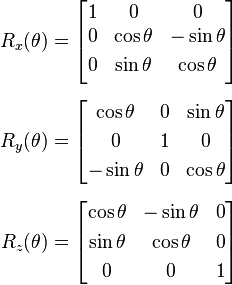
\includegraphics[scale=0.5]{matriceRotation.png}
\caption{\label{hierachical} Illustration des matrices de rotations en x, y et z}
\end{figure}

Pour plus d'informations sur les quaternions, voir \cite{quaternion} et pour plus d'informations sur les matrices de rotations, voir \cite{matrice}.


\subsection{Outils utilisés dans le projet}  \label{outilsUtilise}

\subsubsection{Framework .NET}
Le \textit{Framework .NET} est utilisé par Windows. Il s'appuie sur une norme CLI (Common Language Infrasture) qui est indépendante du langage de programmation. Cela permet aux langages compatibles respectant cette norme d'avoir accès à toutes les bibliothèques disponibles sur l'environnement d'exécution. Il fournit une approche unifiée pour la conception d'applications Windows et Web.

\subsubsection{Visual Studio 2013}
\textit{Visual Studio 2013} est un logiciel de développement pour Windows conçue par Microsoft. Il permet de générer des applications Web ASP.NET, des services Web XML et bien d'autres. \\
Les langages tel que \textit{Visual Basic, Visual C++, Visual C\# et Visual J\#} permettent de mieux tirer parti des fonctionnalités du \textit{Framework .NET}.


\subsubsection{SDK 1.8 du Kinect v1}
Le \textit{SDK 1.8 pour Windows} fournit des outils et une API pour implémenter une application utilisant le \textit{Kinect}. \\

Le \textit{SDK 1.8} est la mise à jour des anciens SDK. En plus des autres SDK, il contient :
\begin{itemize}
	\item \textbf{Kinect Background Removal :} fournit un écran vert pour une seule personne.
	\item \textbf{Webserver for Kinect Data Streams : }permet l'envoi des informations captées par le \textit{Kinect} sur une page Web utilisant les \textit{WebSockets}.
	\item \textbf{Color Capture and Camera Pose Finder for Kinect Fusion :} permet de scanner un objet 3D puis de le modéliser en utilisant le \textit{Kinect}.
	\item Beaucoup d'exemples.
\end{itemize}
Pour plus d'informations sur les différents \textit{SDK du Kinect v1}, Voir \cite{SDKKinectv1}.  \\

Ce SDK est le dernier que Windows a sorti pour le \textit{Kinect v1}. Quand le \textit{Kinect v2} est sorti le SDK 2.0 a pris le relais. \\

\pagebreak
\paragraph{Exemple d'utilisation \\ }
L'exemple qui suit capte la personne devant le Kinect. Il est séparé en deux parties : l'initialisation du \textit{Kinect} et la capture des données.

\lstset{language=[Sharp]C,
basicstyle=\footnotesize,
backgroundcolor=\color{backcolour}, 
captionpos=b,
frame=lines, % Oberhalb und unterhalb des Listings ist eine Linie
showspaces=false,
showtabs=false,
breaklines=true,
showstringspaces=false,
breakatwhitespace=true,
escapeinside={(*@}{@*)},
commentstyle=\color{greencomments},
morekeywords={partial, var, value, get, set},
keywordstyle=\color{bluekeywords},
stringstyle=\color{redstrings}
}
\begin{lstlisting}
//Initialisation du Kinect
KinectSensor kinect = null;

void StartKinectST()
{
	// Get first Kinect Sensor
	kinect = KinectSensor.KinectSensors.FirstOrDefault(s => s.Status == KinectStatus.Connected); 
	kinect.SkeletonStream.Enable(); // Enable skeletal tracking
	
	// Allocate ST data
	skeletonData = new Skeleton[kinect.SkeletonStream.FrameSkeletonArrayLength]; 

	// Get Ready for Skeleton Ready Events
	kinect.SkeletonFrameReady += new EventHandler<SkeletonFrameReadyEventArgs>(kinect_SkeletonFrameReady); 

	// Start Kinect sensor
	kinect.Start(); 
}

//Capture des donnees
private void kinect_SkeletonFrameReady(object sender, SkeletonFrameReadyEventArgs e)
{
  // Open the Skeleton frame
  using (SkeletonFrame skeletonFrame = e.OpenSkeletonFrame()) 
  {
  	// check that a frame is available
	if (skeletonFrame != null && this.skeletonData != null) 
	{
	  // get the skeletal information in this frame
	  skeletonFrame.CopySkeletonDataTo(this.skeletonData);
	  
	  // draw the skeletons
	  foreach (Skeleton skeleton in this.skeletonData)
      {
          if (skeleton.TrackingState == SkeletonTrackingState.Tracked)
          {
              DrawSkeletonPosition(skeleton.Position);
          }
      } 
	}
  }
}

\end{lstlisting}

\subsubsection{Socket IO C\# Client}
\textit{Socket IO C\# Client} (socket.io-csharp-client) est un projet disponible sur \textit{GitHub} \cite{SocketIOCSharp}. Il permet de faire communiquer un programme C\# avec un \textit{serveur NodeJS}. Il utilise le \textsf{package} \textit{NuGet}, un gestionnaire de \textsf{packages} sur \textit{Visual Studio}. Il permet d'ajouter des \textsf{packages} à une application \textit{Visual Studio}. \\
Il permet de créer et modifier des \textsf{packages} et fournit un grand nombre de \textsf{packages} pour Windows. \\
Il utilise également \textit{WebSocket4Net}, un autre projet \textit{GitHub} \cite{WebSocket4Net} qui permet d'utiliser les \textit{WebSockets} client.\\

Ce projet est utilisé pour transmettre les données captées au client HTML. Il a permis de résoudre le problème décrit au chapitre~\ref{problemes}

\paragraph{Exemple d'utilisation \\ }
L'exemple ci-dessous n'utilise pas le \textit{Kinect}. Il montre comment utiliser \textit{SocketIOC\# Client} dans un projet.

\lstset{language=[Sharp]C,
basicstyle=\footnotesize,
backgroundcolor=\color{backcolour}, 
captionpos=b,
frame=lines, % Oberhalb und unterhalb des Listings ist eine Linie
showspaces=false,
showtabs=false,
breaklines=true,
showstringspaces=false,
breakatwhitespace=true,
escapeinside={(*@}{@*)},
commentstyle=\color{greencomments},
morekeywords={partial, var, value, get, set},
keywordstyle=\color{bluekeywords},
stringstyle=\color{redstrings}
}

\begin{lstlisting}
using System;
using SocketIO.Client;

namespace SimpleClient
{   
   class Example
   {
      static void Main()
      {
         var io = new SocketIOClient();

         var socket = io.Connect("http://localhost:3000/");

         socket.On("data", (args, callback) =>
         {
            Console.WriteLine("Server sent:");

            for (int i = 0; i < args.Length; i++)
            {
               Console.WriteLine("[" + i + "] => " + args[i]);
            }
         });

         string line;

         while ((line = Console.ReadLine()) != "q")
         {
            socket.Emit("data", line);
         }
      }
   }
}
\end{lstlisting}


%%%%%%%%%%%%%%%%%%%%%%%%%%%%%%%%%%%%%%%%%%%%%%%%%%%%%%%%%%%%%%%%%%%%%%%%%%%%%%%%%%%%%%%%%%%%%%%%%%%%%%%%%%%%%%%%%%%%%%%%%%%

\pagebreak
\section{Technologies 3D}  \label{technologies}
Ce projet nécessite la visualisation de scènes 3D et la modélisation de scènes 3D. Le \textit{Framework X3DOM} permet à ce projet de ne pas être dépendant du système d'exploitation du \textsf{smartphone} car il suffit d'un accès internet. Cette solution permet à n'importe qui de pouvoir facilement tester et utiliser ce projet. Il permet également d'avoir plusieurs clients, un testeur et une visionner. \\ 

Les logiciels de modélisations 3D \textit{Blender et Cinema4D} ont été utilisés pour modéliser des scènes 3D. \textit{Blender} permet d'exporter les scènes 3D en format X3D supporté par \textit{X3DOM}. Le personnage 3D a été modélisé en utilisant le logiciel \textit{MakeHuman}. Plus d'informations sur la modélisation des scènes du projet au chapitre~\ref{implementation}.

\subsection{X3DOM}  \label{x3dom}
\begin{figure}[H]
\flushright
   
\includegraphics[scale=0.2]{x3domLogo.png}
\end{figure}

\textit{X3DOM} est un \textsf{Framework} open source qui permet d'afficher des scènes 3D sur une page Web. \textit{X3DOM} est la composition entre \textsf{X3D} (Extensible 3D Graphics) et \textsf{DOM} (Document Object Model). Il permet d'intégrer X3D dans le DOM et d'utiliser, par exemple un listener d'événements ou les modifications du HTML dynamiquement avec \textsf{JavaScript}. \\

L'utilisation de \textit{X3DOM} au lieu d'une autre librairie apporte certains avantages :
\begin{itemize}
\item pas besoin d'un plugin pour afficher les scènes 3D;
\item étant basé sur un nouveau profil HTML de l'ISO Standard X3D, il est conforme au standard;
\item il existe une large communauté de développeurs;
\item utilisation du HTML et DOM plutôt que d'apprendre à programmer avec une nouvelle API;
\item il suffit de télécharger et inclure les documents CSS et \textsf{JavaScript} pour l'utiliser.\\
Pour plus d'informations sur \textit{X3DOM} voir \cite{X3DOM}, sur X3D voir section~\ref{x3d} ou sur DOM voir \cite{DOM}.

\end{itemize}

\paragraph{Exemple d'utilisation \\ }
Afin d'ajouter de la 3D sur une simple page HTML, il faut impérativement avoir les éléments suivants : 

\begin{itemize}
\item le fichier de script x3dom.js permettant de manipuler la 3D,
\item le fichier de style x3dom.css pour le placement des éléments dans la scène 3D.\\

\end{itemize}
\pagebreak
Voici un exemple très simple d'utilisation de \textit{X3DOM}. Dans cet exemple, un cône, un cube et une sphère sont créés sur la même ligne et bougent tous en même temps.

\lstset{style=mystyle} 
\begin{lstlisting}[language=Html]
<html> 
   <head>
    <meta http-equiv="X-UA-Compatible" content="IE=edge"/> 
     <title>My first X3DOM page</title> 
     <script src='http://www.x3dom.org/download/x3dom.js'> </script> 
     <link rel='stylesheet' type='text/css' 
           href='http://www.x3dom.org/download/x3dom.css'/> 
   </head> 
   <body> 
	 <x3d width='500px' height='400px'> 
	   <scene> 
		<shape> 
		   <appearance> 
			 <material diffuseColor='1 0 0'></material> 
		   </appearance> 
		   <box></box> 
		</shape> 
		<transform translation='-3 0 0'> 
		  <shape> 
			 <appearance> 
			   <material diffuseColor='0 1 0'></material> 
			 </appearance> 
			 <cone></cone> 
		  </shape> 
		</transform> 
		<transform translation='3 0 0'> 
		  <shape> 
			 <appearance> 
			   <material diffuseColor='0 0 1'></material> 
			 </appearance> 
			 <sphere></sphere> 
		  </shape> 
		</transform> 
	   </scene> 
	</x3d> 
   </body> 
</html> 
\end{lstlisting}

Voici le résultat de cet exemple : 
\begin{figure}[H]
\centering
	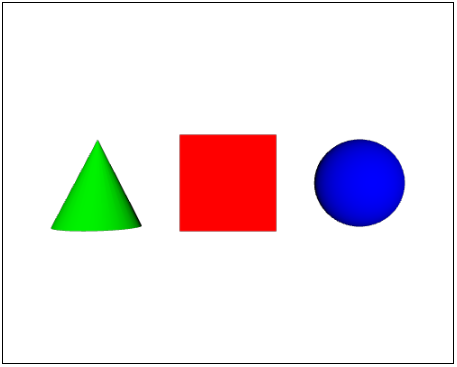
\includegraphics[scale=0.5]{exempleX3DOM.png}
\end{figure}

\subsection{Logiciels 3D - Blender, MakeHuman et Cinema4D}  \label{logiciel3D}

\subsubsection{Blender}
\textit{Blender} est un logiciel de modélisation, d'animation et de rendu 3D développé par la \textsf{Fondation Blender}. \\
\textit{X3DOM} prévoit une balise utilisant un format que seul \textit{Blender} met à disposition en exportation au format X3D. 

\subsubsection{Format x3d} \label{x3d}
Le \textit{format X3D} (Extensible 3D) est un format de fichier graphique et multimédia orienté 3D.\\
X3D s'appuie sur une structure de type graphe de scène. \\
X3D est un couplage entre une page HTML et un objet \textit{Blender} \\
Le format X3D est très similaire à \textit{X3DOM}. Un exemple du format X3D et un exemple de \textit{X3DOM} sont placés en annexes afin de voir la comparaison (pour plus d'informations sur X3D voir \cite{X3D}).

\subsubsection{MakeHuman}
\textit{MakeHuman} est un logiciel libre de modélisation 3D de corps humains. Les modèles générés sont destinés à être utilisés sur \textit{Blender} ou un autre logiciel 3D. \\

Il dispose d'une interface simple permettant de créer facilement un corps humain de n'importe quel type et en modifiant et personnalisant toutes les caractéristiques du corps humain.

\subsubsection{Cinema4D}
\textit{Cinema4D} est un logiciel de création 3D développé par \textsf{Maxon}. Il permet la modélisation, le texturage, l'animation et le rendu d'objets 3D.

%%%%%%%%%%%%%%%%%%%%%%%%%%%%%%%%%%%%%%%%%%%%%%%%%%%%%%%%%%%%%%%%%%%%%%%%%%%%%%%%%%%%%%%%%%%%%%%%%%%%%%%%%%%%%%%%%%%%%%%%%%%

\pagebreak 
\section{Serveur Web Virtual-Vertigo en NodeJS}  \label{serveur}
Dans le cadre de ce projet, un serveur est nécessaire pour transmettre les informations captées par le \textit{Kinect} aux clients HTML. \\

\begin{figure}[H]
	\centering
		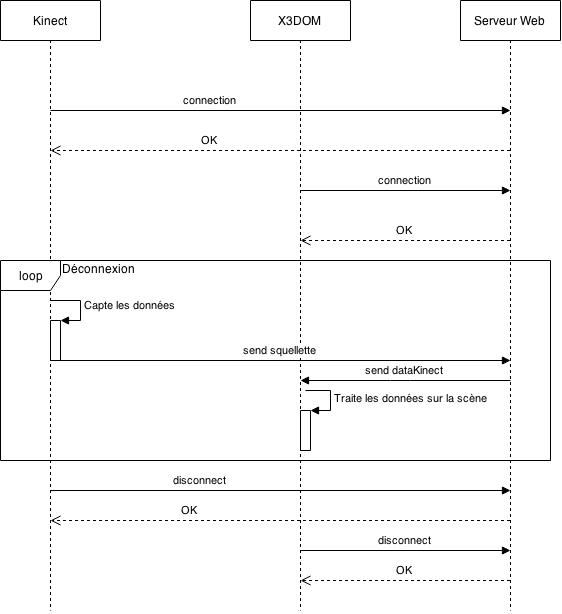
\includegraphics[scale=0.7]{DiagrammeServeur.jpg}
	\caption{\label{DiagrammeServeur} Diagramme de séquences illustrant la communication avec le serveur}
\end{figure}
Comme vous pouvez le voir sur ce diagramme de séquences~\ref{DiagrammeServeur}, le \textit{Kinect} et le client HTML se connectent au serveur. Puis le \textit{Kinect} envoie toutes les secondes les informations captées et dès que le serveur reçoit les données du \textit{Kinect}, il les retransmet directement aux clients HTML qui va les interpréter sur la scène 3D. Tout ceci s'effectue jusqu'à la déconnexion du \textit{Kinect} et des clients HTML.\\

Le \textit{serveur Web Virtual-Vertigo} est un serveur Web utilisant les \textit{WebSockets} pour les communications. Lors du projet de semestre sur le même thème, un travail préliminaire a permis de choisir entre \textit{MeteorJS} et \textit{NodeJS}. \textit{MeteorJS} est un \textsf{Framework} permettant de construire des sites Web modernes et d'implémenter automatiquement un serveur Web, sans avoir besoin de gérer quoi que ce soit. Cependant, \textit{NodeJS} a été choisi car on avait besoin de plus de contrôle sur l'implémentation du serveur.\\
Pour plus d'informations sur les \textit{WebSockets} voir \cite{websocket}, sur \textit{MeteorJs} voir \cite{MeteorJS}.

\subsection{NodeJS}
\begin{figure}[H]
	\flushright
   		
\includegraphics[scale=0.1]{nodeLogo.png}
\end{figure}
\textit{NodeJS} est un \textsf{Framework} logiciel et évènementiel en \textsf{JavaScript}. Il contient une bibliothèque de serveur HTTP, ce qui permet de faire tourner et de mieux contrôler un serveur Web sans avoir besoin d'un logiciel externe. \\
L'avantage de ce \textsf{Framework} est qu'il permet d'ajouter plusieurs modules permettant de manipuler les services Web plus facilement (par exemple l'utilisation de \textit{WebSockets} avec le module \textit{Socket.io}). Ces modules sont disponibles car il utilise \textit{npm}, un gestionnaire de \textsf{packages} officiel pour \textit{NodeJS} qui permet d'installer des applications disponibles sur le dépôt \textit{npm}. \\
A noter que la plupart des projets disponibles sur le dépôt \textit{npm} sont des projets implémentés par un utilisateur qui a voulu partager son travail en le mettant à disposition sur \textit{GitHub} (our plus d'informations sur \textit{NodeJS}, voir \cite{NodeJS}).

\paragraph{Exemple d'utilisation \\}
NodeJS contient deux modules déjà installés :
\begin{itemize}
\item http : module permettant de créer un serveur \textit{http}
\item net : module permettant de créer un serveur \textit{tcp\\}

\end{itemize}

L'exemple qui suit met en place un serveur en utilisant le module http. 

\lstset{style=mystyle} 
\begin{lstlisting}[language=JavaScript]
// Load the http module to create an http server.
var http = require('http');

// Configure our HTTP server to respond with Hello World to all requests.
var server = http.createServer(function (request, response) {
  response.writeHead(200, {"Content-Type": "text/plain"});
  response.end("Hello World\n");
});

// Listen on port 8000, IP defaults to 127.0.0.1
server.listen(8000);

// Put a friendly message on the terminal
console.log("Server running at http://127.0.0.1:8000/");
\end{lstlisting}


A noter qu'un tutoriel contenant les instructions pour l'installation et l'utilisation de \textit{NodeJS} et \textit{npm} est disponible en annexe.

\subsection{Module ExpressJS}
ExpressJS installé avec npm, permet de créer et gérer une application Web plus facilement parce qu'il s'occupe de création du serveur, il suffit donner une adresse ip et il le crée pour nous. Dans ce projet, il est utilisé gérer les parties accessibles depuis le serveur. L'utilisation d'ExpressJS a permis de mettre en place l'architecture décrite dans le chapitre précédent.\\

\paragraph{Exemple d'utilisation \\}
L'exemple suivant crée un serveur local sur le port 3000. Lorsqu'un client se connecte, un message \textsf{Hello World} lui est transmis.\\

\lstset{style=mystyle} 
\begin{lstlisting}[language=JavaScript]
var express = require('express');
var app = express();

app.get('/', function (req, res) {
  res.send('Hello World!');
});

var server = app.listen(3000, function () {

  var host = server.address().address;
  var port = server.address().port;

  console.log('Example app listening at http://%s:%s', host, port);

});
\end{lstlisting}


\subsection{Module Socket.io}
Pour ce projet, les \textit{WebSockets} ont été choisis car ils permettent de communiquer et de partager des données avec plusieurs clients HTML. En effet, pour ce projet, le serveur Web devait recevoir et envoyer des données aux clients sans les traiter. En général l'inverse est utilisé, c'est le client qui transmet des données au serveur qui les traitent. Les \textit{WebSockets} ont permis d'envoyer et de recevoir des données depuis le serveur sans avoir a effectuer un traitement préalable. \\

\textit{Socket.io} est un module installé par npm permettant d'utiliser les \textit{WebSockets}. Il permet de facilement les manipuler que ce soit du côté client ou du côté serveur. Dans ce projet, l'utilisation de \textit{SocketIOC\# Client} a nécessité d'utiliser la version 0.9 de \textit{Socket.io}. \textit{SocketIOC\#} permet d'utiliser les \textit{WebSockets} afin de se connecter et d'envoyer ses informations captées par le \textit{Kinect} puis de renvoyer au client HTML. Le module \textit{Socket.io} utilise une syntaxe précise qui doit être respectée du côté client et du côté serveur: 
\begin{itemize}
\item lancement du serveur (seulement pour le serveur) : \texttt{io.listen(\textit{adresse ip du serveur});}
\item l'attente de connexions (seulement pour le serveur) : \texttt{io.sockets.on('connection', \\
function(socket)$\{$ \textit{réception et envoi de données}$\});$}
\item connexion au serveur (seulement pour le client) : \texttt{socketIO.connect(\textit{adresse ip et port du serveur});}
\item la réception de données : \texttt{socket.on(\textit{label de l'envoi}, function(data)$\{$\textit{traitement des données reçue}$\});$}
\item l'envoi de données : \texttt{socket.emit(\textit{label de l'envoi}, \textit{données});}
\end{itemize}
Pour plus d'informations, voir \cite{SocketIO}.\\

\paragraph{Exemple d'utilisation \\}
L'exemple suivant est un chat entre les clients connectés. Cet exemple utilise également le module \textit{ExpressJS} parce que la transmission des messages entre les clients est gérée par un serveur. Lors de la réception d'un message, le serveur le transmet à tous les clients connectés. \\
Cet exemple contient deux parties, un client HTML et un serveur.

\lstset{style=mystyle} 
\begin{lstlisting}[language=JavaScript]
\\ Serveur
var app = require('express')();
var http = require('http').Server(app);
var io = require('socket.io')(http);

app.get('/', function(req, res){
  res.sendFile(__dirname + '/index.html');
});

io.on('connection', function(socket){
  socket.on('chat message', function(msg){
    io.emit('chat message', msg);
  });
});

http.listen(3000, function(){
  console.log('listening on *:3000');
});
\end{lstlisting}


\lstset{style=mystyle} 
\begin{lstlisting}[language=Html]
\\ Client HTML
<!doctype html>
<html>
  <head>
    <title>Socket.IO chat</title>
    <script src="https://cdn.socket.io/socket.io-1.2.0.js"></script>
    <script src="http://code.jquery.com/jquery-1.11.1.js"></script>
  </head>
  <body>
    <ul id="messages"></ul>
    <form action="">
      <input id="m" autocomplete="off" /><button>Send</button>
    </form>
    <script>
      var socket = io();
      $('form').submit(function(){
        socket.emit('chat message', $('#m').val());
        $('#m').val('');
        return false;
      });
      socket.on('chat message', function(msg){
        $('#messages').append($('<li>').text(msg));
      });
    </script>
  </body>
</html>
\end{lstlisting}

\chapter{Implémentation} \label{implementation}
Ce chapitre décrit l'implémentation de l'application \textit{Virtual-Vertigo}. Des illustrations et des extraits de codes commentés ont été insérés afin de rendre les explications plus claires.

%%%%%%%%%%%%%%%%%%%%%%%%%%%%%%%%%%%%%%%%%%%%%%%%%%%%%%%%%%%%%%%%%%%%%%%%%%%%%%%%%%%%%%%%%%%%%%%%%%%%%%%%%%%%%%%%%%%%%%%%%%%

\section{Serveur Virtual-Vertigo}   \label{serveur2}
Le \textit{serveur NodeJS} mis en place utilise les \textit{modules ExpressJS et Socket.io}. Le \textit{module ExpressJS} a permis de créer le serveur Web, de rediriger les clients se connectant au serveur et de rendre les fichiers nécessaires publics. Le \textit{module Socket.io} a permis de créer un serveur utilisant les \textit{WebSockets} avec le serveur Web crée avec le module \textit{ExpressJS}. De plus, il permet de réceptionner les informations du \textit{Kinect} et de les renvoyer aux clients connectés. 

\lstset{style=mystyle} 
\begin{lstlisting}[language=JavaScript]
var express = require("express"), app = express(),
	server = require('http').createServer(app);

// redirection on /public who content the files 
app.use(express.static(__dirname + '/public'));

server.listen(3000, function(){// launch the server
  console.log('listening on *:3000');
});

//create the server socket using the server created with express
var io = require('socket.io').listen(server, { 'destroy buffer size': Infinity });
io.set('log level', 1);

//wait for the connections
io.sockets.on('connection', function(socket){
	console.info('Client connected');	
	// reception of datas captured by the kinect
	socket.on("squelette", function(json){
		io.sockets.emit("dataKinect", json);
	});
	socket.on("orientation", function(start, end, rotation){
		var json = {"start" : start, "end" : end, "rotation" : rotation };
		io.sockets.emit("boneOrientation", json);
	});
	socket.on('disconnect', function() {
		console.info('Client is gone');
	});
});
\end{lstlisting}

Ci-dessous un schéma illustrant l'échange de données entre le \textit{serveur Web Virtual-Vertigo}, les clients HTML et le Kinect.
\begin{figure}[H]
\centering
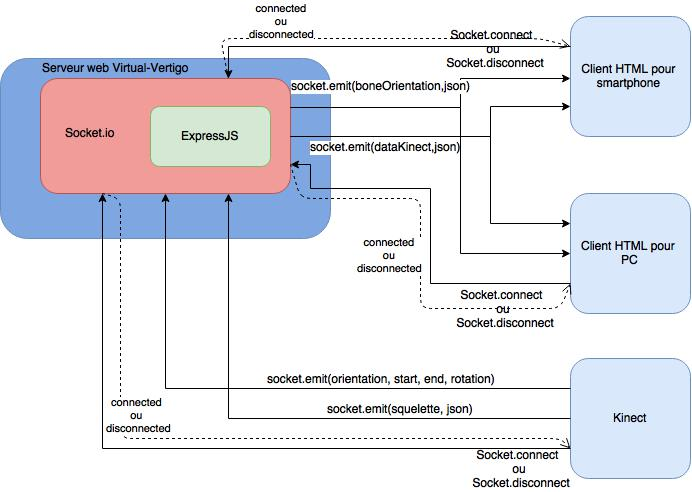
\includegraphics[scale=0.65]{serveur.jpg}
\caption{\label{schemaServeur} Illustration des échanges de données entre serveur, clients HTML et Kinect}
\end{figure}


%%%%%%%%%%%%%%%%%%%%%%%%%%%%%%%%%%%%%%%%%%%%%%%%%%%%%%%%%%%%%%%%%%%%%%%%%%%%%%%%%%%%%%%%%%%%%%%%%%%%%%%%%%%%%%%%%%%%%%%%%%%
\pagebreak
\section{Données provenant du Kinect}  \label{donnees}
Cette section décrit comment les données provenant du \textit{Kinect} ont été interprétées.

\subsection{Capture des données}  \label{capture}
La capture des données du \textit{Kinect} a été effectuée en C\# avec \textit{Visual Studio 2013}. Elle a été effectuée en plusieurs étapes : 
\lstset{language=[Sharp]C,
basicstyle=\footnotesize,
backgroundcolor=\color{backcolour}, 
captionpos=b,
frame=lines, % Oberhalb und unterhalb des Listings ist eine Linie
showspaces=false,
showtabs=false,
breaklines=true,
showstringspaces=false,
breakatwhitespace=true,
escapeinside={(*@}{@*)},
commentstyle=\color{greencomments},
morekeywords={partial, var, value, get, set},
keywordstyle=\color{bluekeywords},
stringstyle=\color{redstrings}
}

\begin{enumerate}
\item La connexion au \textit{serveur NodeJS} utilisant \textit{SocketIOC\# Client}.
\begin{lstlisting}
private static bool InitializeConnection(){
	var io = new SocketIOClient();
	socket = io.Connect("http://localhost:3000/");
	
	if (io.Connected)
		Console.WriteLine("kinect connected to server"); 
	else
		Console.WriteLine("failed to connect to server");
}
\end{lstlisting}

\item L'initialisation du \textit{Kinect}.
\begin{lstlisting}
private static void InitilizeKinect(){
	sensor = KinectSensor.KinectSensors.SingleOrDefault();
	if (sensor != null)
	{
		sensor.SkeletonStream.TrackingMode = SkeletonTrackingMode.Default;
		sensor.SkeletonStream.Enable(new TransformSmoothParameters()
		{
			Smoothing = 0.5f,
			Correction = 0.5f,
			Prediction = 0.5f,
			JitterRadius = 0.05f,
			MaxDeviationRadius = 0.04f
		});
		sensor.AllFramesReady += Sensor_AllFramesReady;

		sensor.Start();
		Console.WriteLine("sensor started");
	}
}
\end{lstlisting}

\item La capture et l'envoi de la position de chaque articulation captée du squelette.
\begin{lstlisting}
static void Sensor_AllFramesReady(object sender, AllFramesReadyEventArgs e) {
	using (var frame = e.OpenSkeletonFrame()) {
		if (frame != null){
			frame.CopySkeletonDataTo(skeletons);

			foreach (Skeleton skeleton in skeletons)
			{
				if (skeleton.TrackingState == SkeletonTrackingState.Tracked)
				{
					socket.Emit("squelette", skeleton.Joints);
					[...]
				}
			}
		}
	}
}
\end{lstlisting}

\item La récupération et l'envoi de l'orientation des mains afin de pouvoir voir la rotation de la main lors de la simulation.
\begin{lstlisting}
static void Sensor_AllFramesReady(object sender, AllFramesReadyEventArgs e) {
	[...]
	foreach (BoneOrientation orientation in skeleton.BoneOrientations)
	{
		if (orientation.StartJoint == JointType.WristLeft || orientation.StartJoint == JointType.WristRight)
				socket.Emit("orientation", orientation.StartJoint, orientation.EndJoint, orientation.AbsoluteRotation.Quaternion);
		}
	} 
}
\end{lstlisting}
\end{enumerate}

\subsection{Format des données}  \label{format}
Les données de positions envoyés au serveur sont au \textsf{format json} et sont des valeurs de la scène réelle. Les données sont envoyées dans un tableau où chaque élément est un \textsf{objet json} contenant les informations: 
\begin{itemize}
\item la valeur du point capté
\item le vecteur de position
\item l'état de l'articulation (captée, inférée ou non-captée), cette information n'est pas utilisée 
\end{itemize}

\begin{figure}[H]
\centering
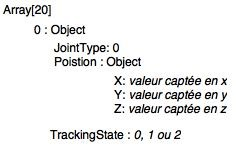
\includegraphics[scale=0.65]{jsonRecu.jpg}
\caption{\label{jsonrecu} Illustration de l'objet json des positions}
\end{figure}

Les données envoyées pour l'\textsf{orientation des mains} sont les suivantes : 
\begin{itemize}
\item le point d'origine, dans notre cas, le poignet
\item le point de fin, dans notre cas, la main
\item le vecteur d'orientation et l'angle de rotation en radians 
\end{itemize}

\begin{figure}[H]
\centering
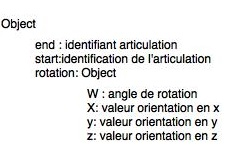
\includegraphics[scale=0.65]{jsonOrientation.jpg}
\caption{\label{jsonrecu} Illustration de l'objet json de l'orientation des mains}
\end{figure}
Pour plus d'informations sur les objets json, voir \cite{json}.

\subsection{Traitement des données} \label{traitement}
Selon le diagramme de séquence~\ref{sequence}, lorsque le serveur reçoit les données du Ki\textit{n}ect, il les renvoie aux clients HTML. Lorsque les clients HTML reçoivent à leur tour les données, celles-ci sont parcourues afin de faire correspondre les valeurs reçues avec une articulation du squelette (voir table des identificateurs d'articulations~\ref{valeurs}). Ces données sont réceptionnées dans un \textsf{nouvel objet json} contenant les informations: 

\begin{itemize}
\item le nom de l'articulation
\item la position x de l'articulation
\item la position y de l'articulation
\item la position z de l'articulation
\end{itemize}

\begin{figure}[H]
\centering
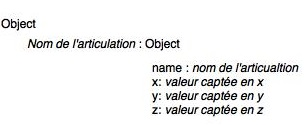
\includegraphics[scale=0.7]{jsonCreer.jpg}
\caption{\label{jsonrecu} Illustration de l'objet json créé avec les positions reçues et leurs articulations}
\end{figure}

A partir de cet \textsf{objet json}, le positionnement de chaque articulation peut être effectué. Au niveau des clients, un membre est représenté par deux sphères reliées par un cylindre. Afin d'adapter ces membres à la taille de chaque personne et d'animer ce personnage virtuel plusieurs étapes sont effectuées : 

\begin{itemize}
\item le calcul de la distance entre deux articulations reliées
\item le positionnement du membre entre les deux articulations
\item l'adaptation de la taille du membre en fonction de la distance calculée
\item le calcul de l'angle entre ses deux articulations en utilisant la fonction \texttt{atan2} (voir section~\ref{atan2})
\item la rotation du membre en fonction de l'angle calculé \\

\end{itemize} 
La description détaillée de chaque étape se trouve à la section~\ref{animation}. \\

Finalement, le déplacement du personnage selon l'avancement de la personne est effectué en se basant sur la position de sa tête. Tout ce traitement est effectué à la réception de chaque information du \textit{Kinect}. En effet, le \textit{Kinect} envoie un \textit{nouvel objet json} cycliquement.\\
Afin de rendre le personnage réaliste, l'ajout de membres réalistes par dessus les cylindres du personnage 3D serait envisageable. 

%%%%%%%%%%%%%%%%%%%%%%%%%%%%%%%%%%%%%%%%%%%%%%%%%%%%%%%%%%%%%%%%%%%%%%%%%%%%%%%%%%%%%%%%%%%%%%%%%%%%%%%%%%%%%%%%%%%%%%%%%%%
\pagebreak
\section{Modélisation de réalité virtuelle} \label{realiteVirtuelle}

\subsection{Création de la scène virtuelle}  \label{creation}
La création de la scène de réalité virtuelle a été réalisée avec \textit{X3DOM} (voir section~\ref{x3dom}). Afin d'ajouter de la 3D sur une simple page HTML, il faut impérativement avoir les fichiers suivants : 

\begin{itemize}
\item Le script x3dom.js permettant de manipuler la 3D
\item Le page de style x3dom.css afin d'utiliser la 3D \\

\end{itemize}

La création de la scène 3D est très simple, elle est basée sur un système de balises. Pour avoir la 3D sur la page, il y a plusieurs balises:

\begin{itemize}
\item la balise principale : \texttt{<x3d>}, 
\item la balise dans laquelle se trouve toute la scène 3D : \texttt{<scene>}, 
\item la balise permettant de définir de type de navigation(\texttt{examine}, \texttt{walk}, \texttt{fly}, etc.) : \texttt{<navigationinfo>},
\item la balise correspondant à la caméra : \texttt{<viewpoint>},
\item la balise permettant de dessiner des éléments 3D directement sur la page HTML : \texttt{<shape>}, 
\item les balises créer l'élément 3D voulu : \texttt{<box>, <sphere>, <cylinder>},
\item la balise permettant d'importer des scène 3D depuis Blender en format X3D : \texttt{<inline>}, 
\item la balise permettant de modifier l'élément 3D : \texttt{<transform>}.
\end{itemize}
Pour en savoir plus sur les balises voir \cite{NodesX3DOM}. \\
 

Chacune des balises utilisées doivent avoir un identifiant afin de pourvoir les manipuler. La manipulation de ces balises consiste à modifier ses attributs. L'accès aux balises s'effectue en \textit{JQuery}. Ci-dessous un exemple d'accès à une balise via son identifiant: 

\lstset{style=mystyle} 
\begin{lstlisting}[language=JavaScript]
$("#"+name).attr("translation");
\end{lstlisting}

Beaucoup de balises sont utilisées tel que \texttt{<navigationInfo>} afin de définir le mode \texttt{examin}. Cependant, seules deux balises utilisées sont modifiées au cours de la simulation. 
\begin{enumerate}
\item La balise \texttt{<transform>} est utilisée pour ses attributs suivants : 

\begin{itemize}
\item \texttt{translation} : déplace les balises se trouvant dans la balise \texttt{<transform>} dans la scène. Par exemple, le déplacement du personnage et de la caméra sur la planche.
\begin{lstlisting}[language=JavaScript]
$("#armature").attr("translation",  (parseFloat(position.head.z) - 4.0) + " 7.3 0");
$("#camera").attr("translation", (parseFloat(position.head.z) - 4.0) + " 8 " + (parseFloat(position.head.x) -0.2) );		
\end{lstlisting}

\item \texttt{rotation} : effectue une rotation sur les balises se trouvant dedans dans la scène virtuelle. Par exemple, la rotation des immeubles à 90 degrés. 
\begin{lstlisting}[language=Html]
<transform id='immeuble' translation='0 0 0' rotation='0 1 0 1.57' >
    <inline url="./blender/vue_semi_finale.x3d"></inline>
 </transform>
\end{lstlisting} 
\end{itemize}

\item La balise \texttt{<viewpoint>} est utilisée pour ses attributs suivants :

\begin{itemize}
\item \texttt{position} : place la caméra aux coordonnées correspondantes. Par exemple, le placement initiale de la vue.
\begin{lstlisting}[language=Html]
<Viewpoint id="vpp" DEF='viewpoint' position="0 0 5" orientation='1 0 0 -0.2' centerOfRotation="0 0 5"  fieldOfView="2.0" ></Viewpoint>	
\end{lstlisting} 

\item \texttt{centerOfRotation} : position correspondant à l'origine lors de la rotation de la vue. Par exemple, l'avancement du personnage sur la planche. 
\begin{lstlisting}[language=JavaScript]	
vp.attr("position", (parseFloat(position.head.x) -0.2) + " " + (parseFloat(position.head.y) -0.2)+ " " + (parseFloat(position.head.z) -0.2));
vp.attr("centerOfRotation", (parseFloat(position.head.x) -0.2) + " " + (parseFloat(position.head.y) -0.2)+ " " + (parseFloat(position.head.z) -0.2));
			
\end{lstlisting}

\item \texttt{orientation} : quaternion correspondant à l'orientation de la caméra dans la vue. Par exemple, le déplacement lors des mouvements de la tête. 
\begin{lstlisting}[language=JavaScript]	
MYAPP.viewpoint.setAttribute("orientation", orientation[0].x + " " + orientation[0].y + " " + orientation[0].z + " " + orientation[1]);
\end{lstlisting}
\end{itemize}

\end{enumerate}


\subsection{Création des immeubles}  \label{immeubles}
Les immeubles ont été crées avec un logiciel 3D \textit{Blender et Cinema4D}. Pour ce projet, deux scène de réalité virtuelle ont été réalisées : \\

\begin{enumerate}

\item Une version basique, implémentée sur \textit{Blender} contient 3 immeubles, une planche et le sol. Elle est illustrée sur la figure~\ref{ModeleBlender} : \\

\begin{figure}[H]
	\centering
		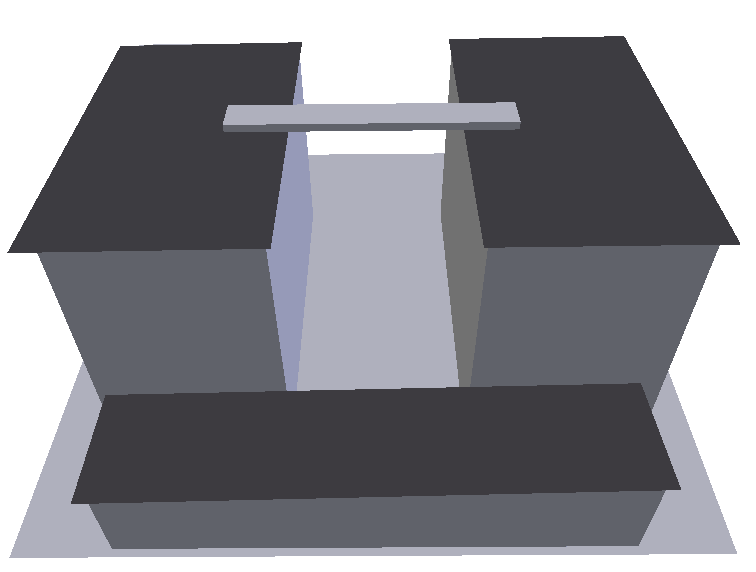
\includegraphics[scale=0.25]{ModeleBlender.png}
	\caption{\label{ModeleBlender} Modèle de vue 3D modélisé sur Blender}
\end{figure}

\item Afin de rendre la vue virtuelle plus réaliste, nous avons contacté \textsc{M. Olivier Donzé}, professeur de la filière architecture de paysage, et son assistant, \textsc{M. Benjamin Dupont-Roy} , qui travaillent sur la modélisation 3D du territoire. \\
La deuxième version,  réalisée par \textsc{M. Benjamin Dupond-Roy}, est plus détaillé et plus réaliste. Elle a été implémentée sur \textit{Cinema4D}. Il a modélisé la rue devant hepia en la personnalisant un peu. Voici quelques vues de son travail : \\

\begin{figure}[H]
   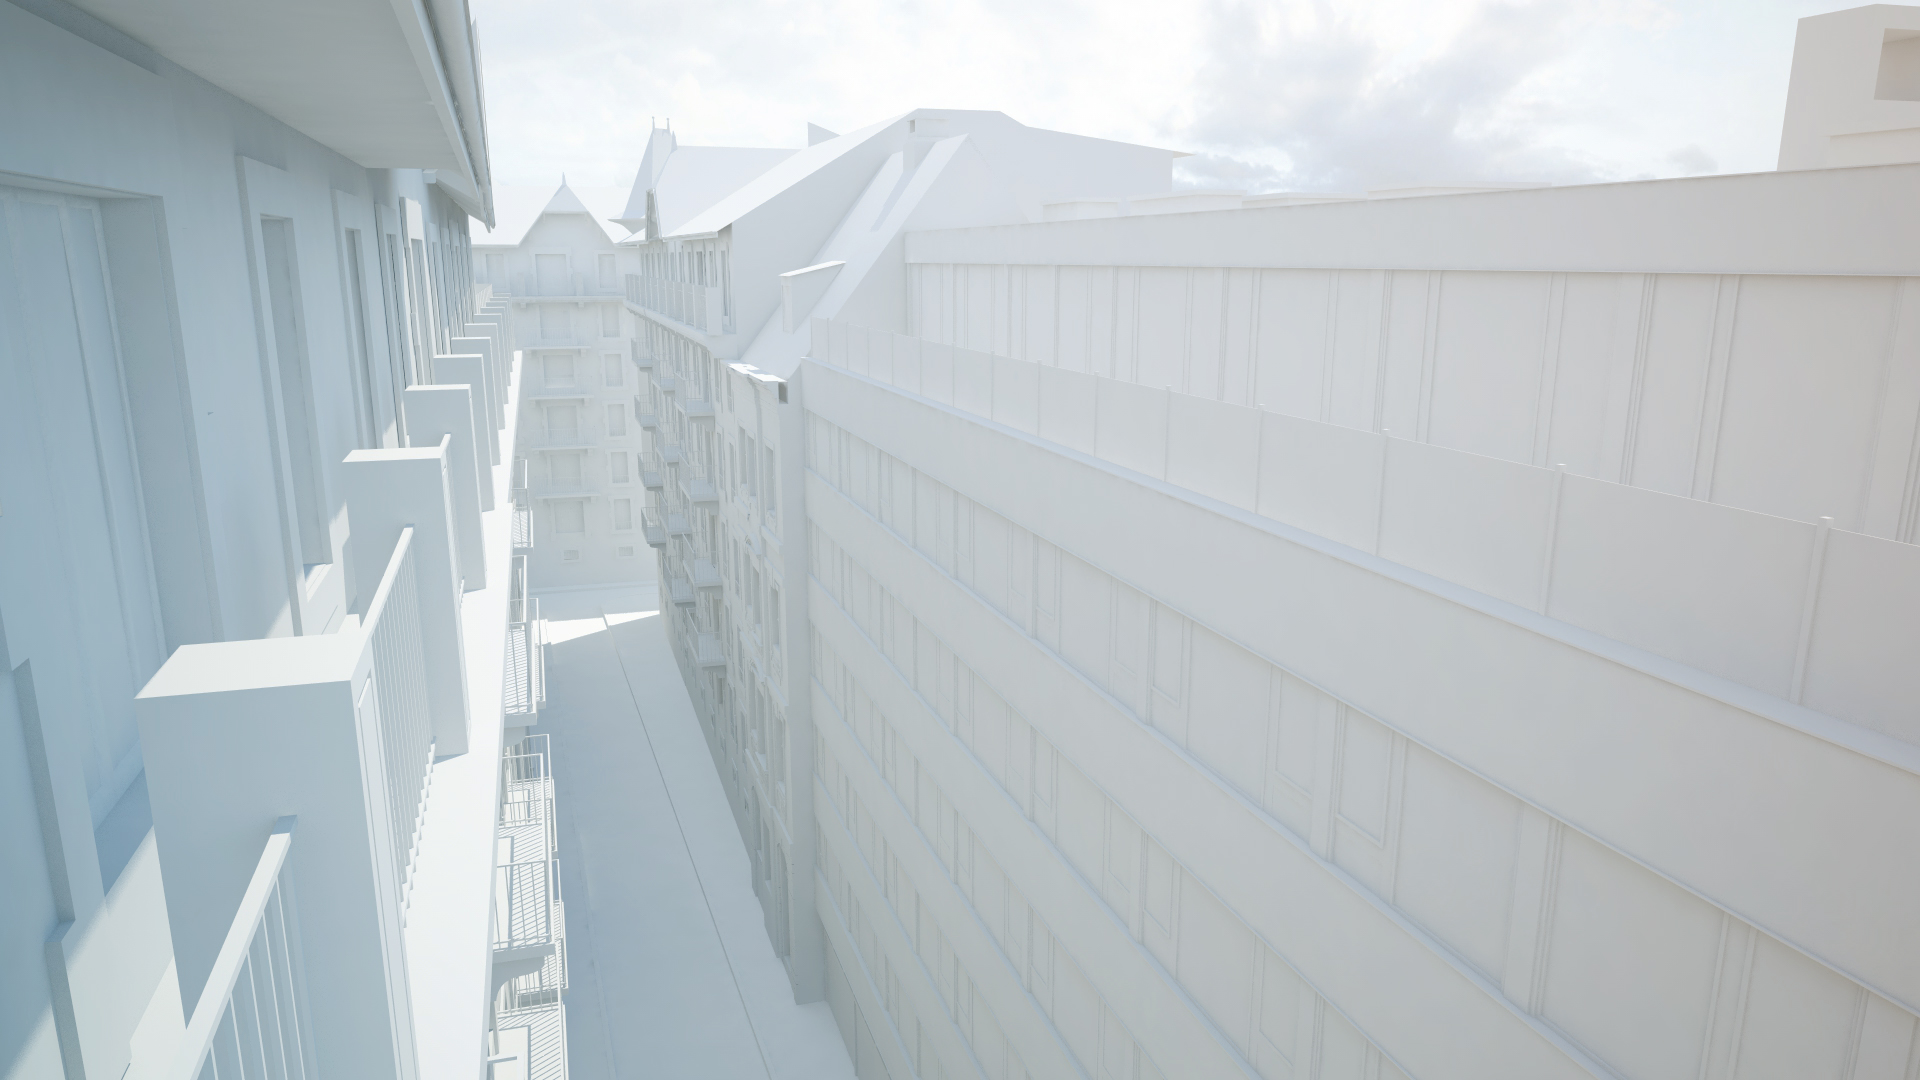
\includegraphics[scale=0.1]{Vue_balcon_OK.jpg}
   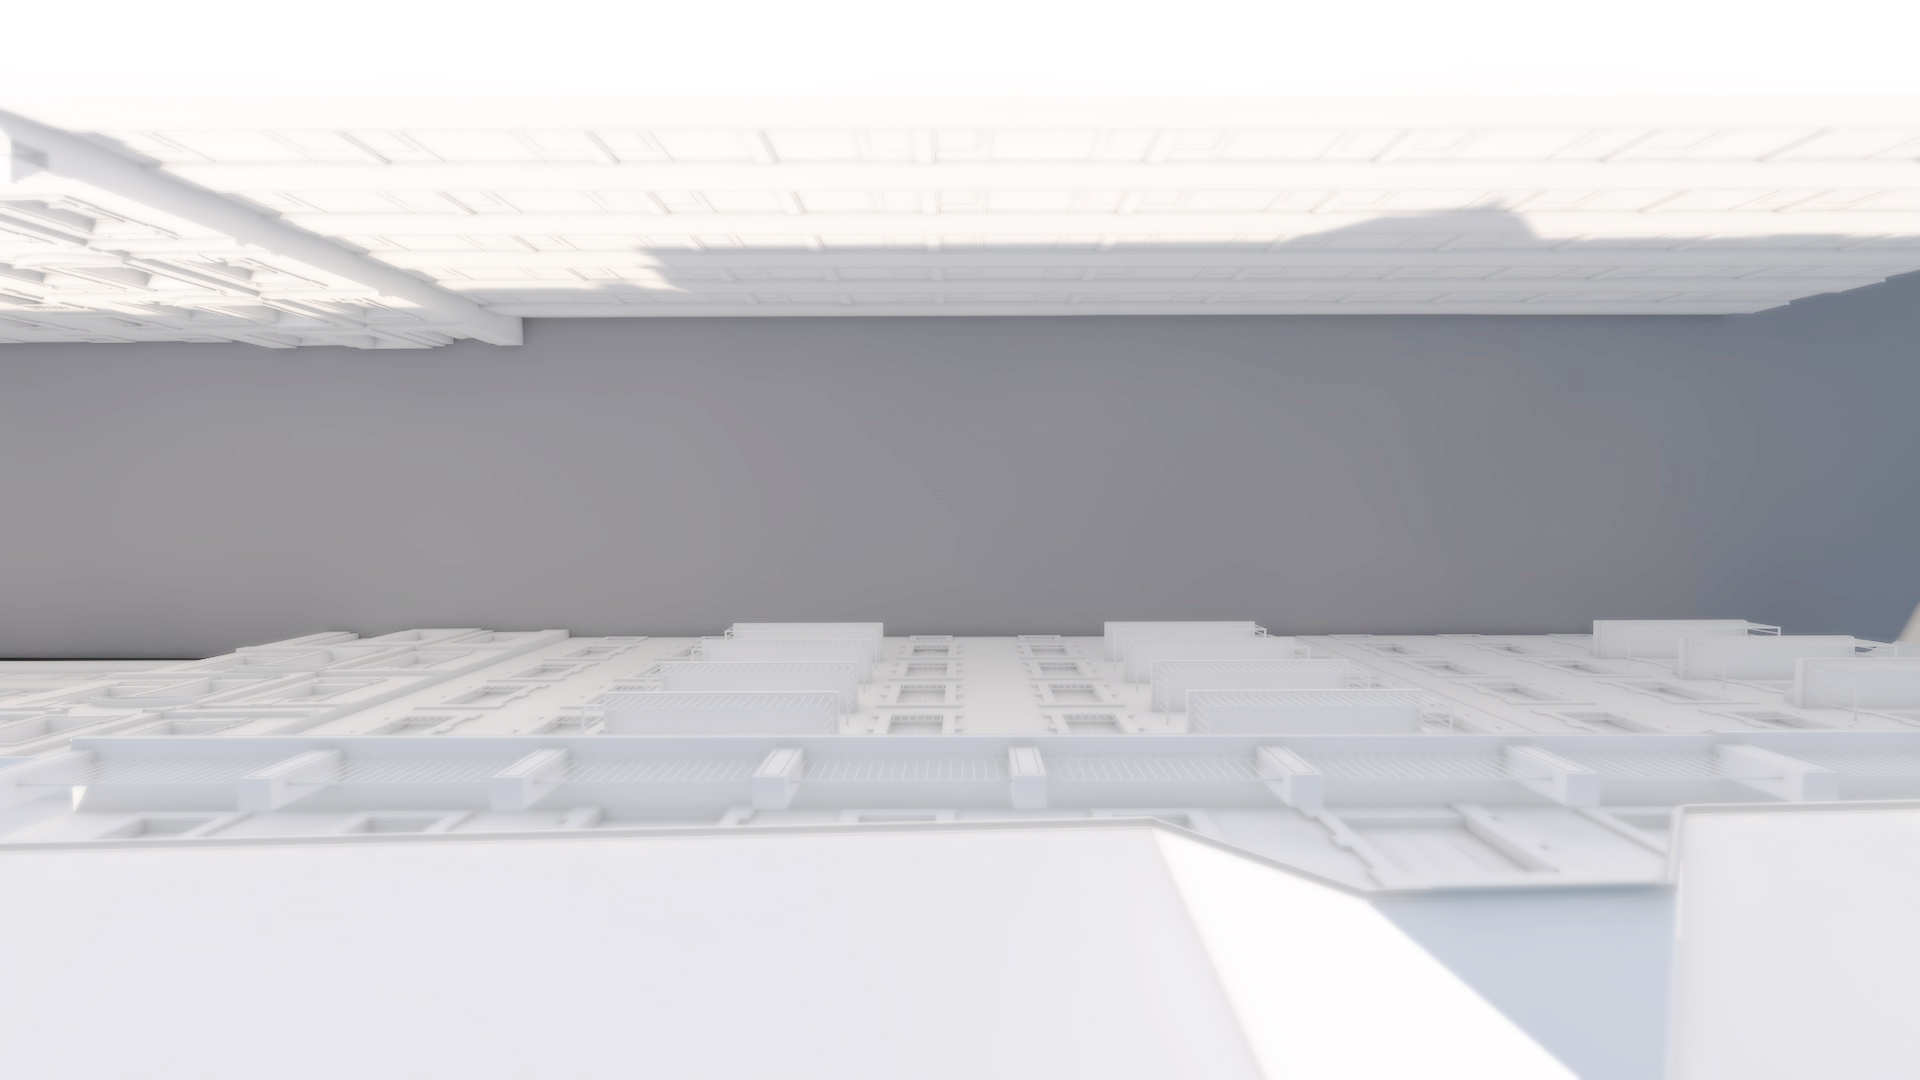
\includegraphics[scale=0.1]{Vue_2_ok.jpg}
   \caption{\label{vue 1 et 2} vue entre immeubles et du dessus}
\end{figure}
\begin{figure}[H]
   \includegraphics[scale=0.1]{Vue_rue_ok.jpg}
   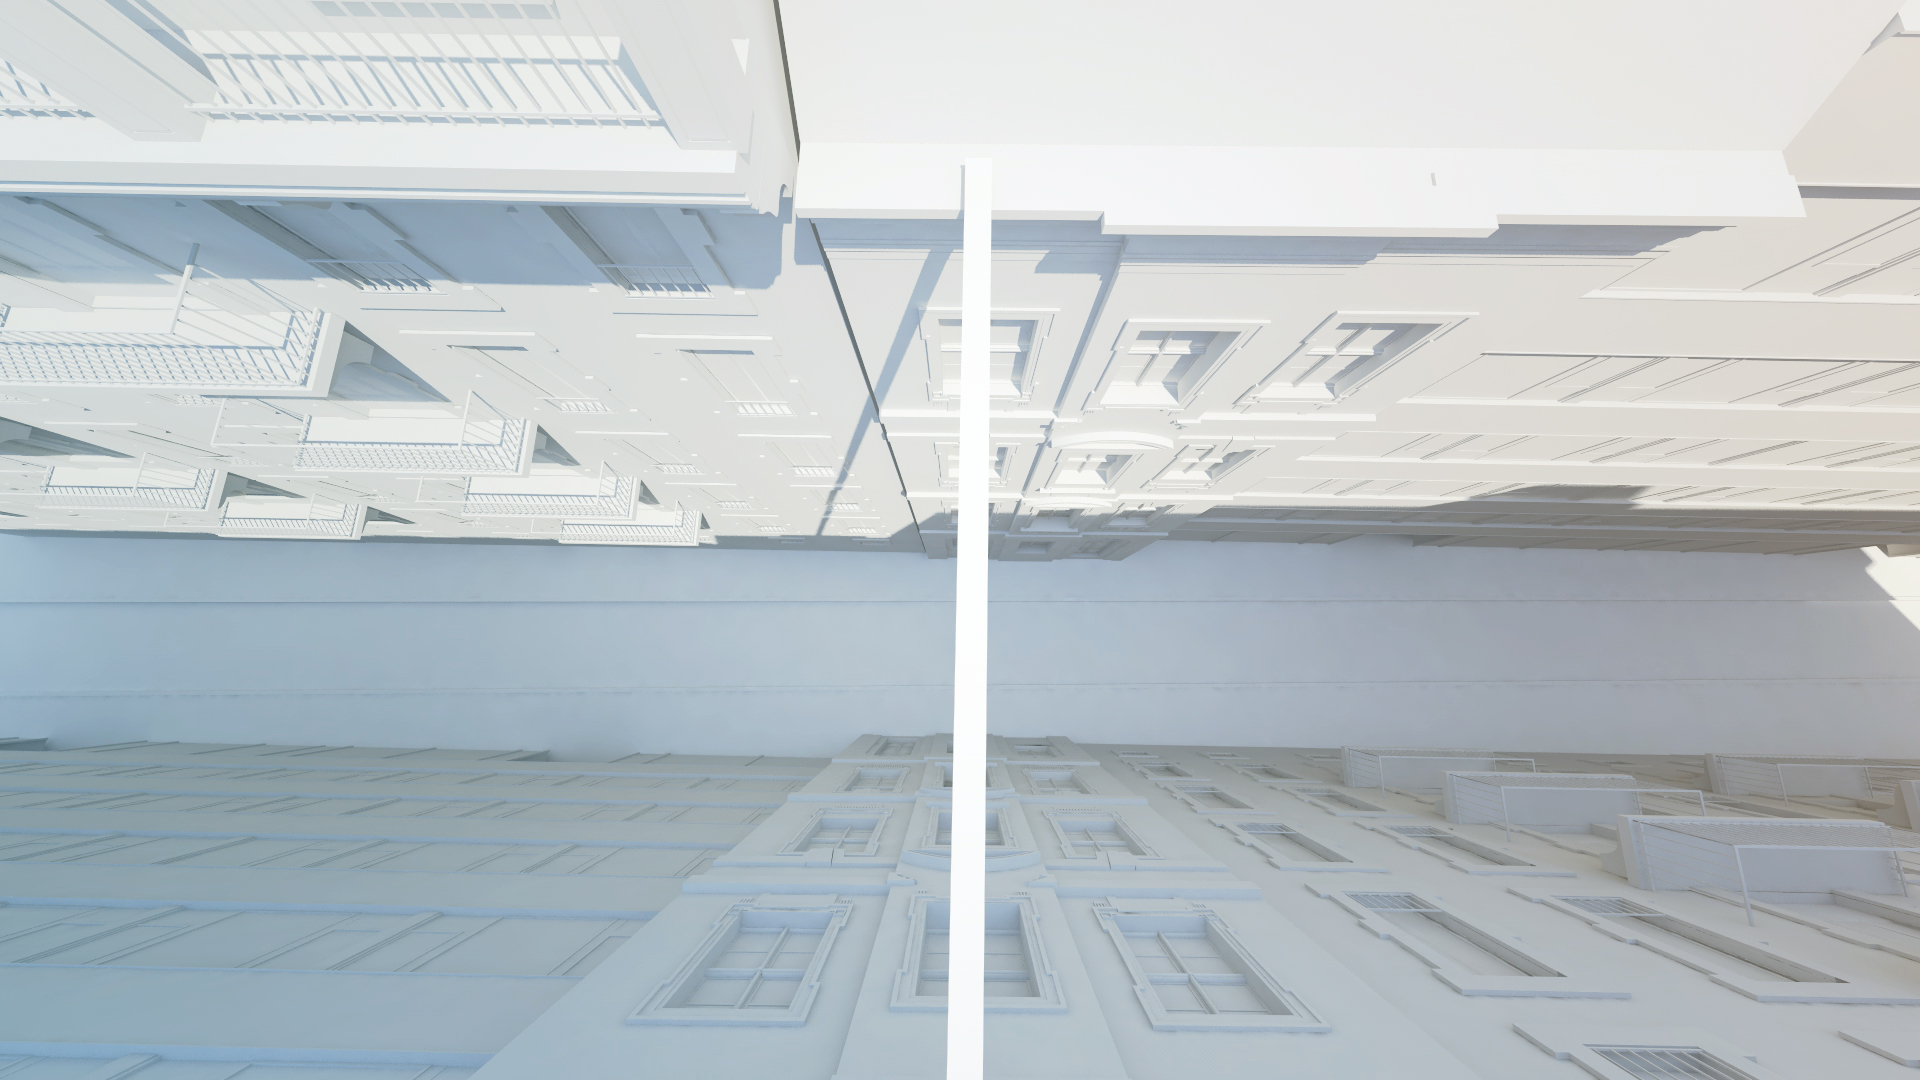
\includegraphics[scale=0.1]{Vue_planche_OK.jpg}
   \caption{\label{vue 3 et 4} vue depuis la rue et depuis la planche}
\end{figure}

\end{enumerate}

\subsection{Création du personnage}  \label{personnages}

La création du personnage a changé plusieurs fois lors de ce projet. Dans un premier temps, une femme avait été modélisée sur \textit{Blender} mais n'étant pas assez réaliste, celle-ci n'a plus été utilisée. \\
Puis, en utilisant \textit{MakeHuman} un homme réaliste a été créé et un squelette lui a été ajouté afin de l'animer si possible.
Cet homme a été utilisé pendant une grande partie du projet mais lorsqu'il a fallu l'animer il ne convenait plus. En effet, un problème d'export sous \textit{Blender} rendait le personnage rigide (pour plus de détails voir section~\ref{animationPersonnage}). \\
Finalement, afin de pouvoir animer un personnage en fonction du \textit{Kinect}, un squelette a été recréé en 3D. L'animation du personnage a été privilégiée par rapport à un rendu réaliste car priorité était de voir ses membres bouger lorsque l'on porte les \textit{Google CardBoard}. \\

Ci-dessous une illustration montrant l'"évolution" du personnage 3D tout au long du projet.
\begin{figure}[H]
	\centering
   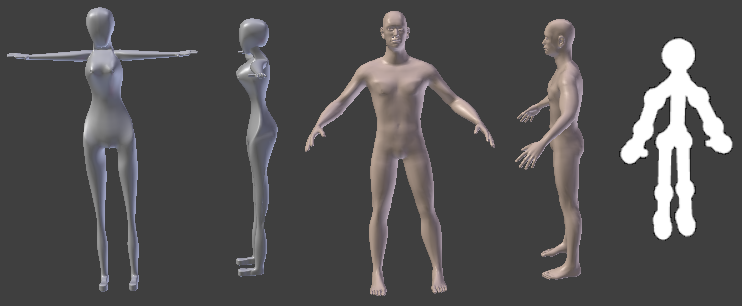
\includegraphics[scale=0.4]{Personnages.png}
   \caption{\label{Evopersonnages} "Evolution" du personnage 3D}
\end{figure}


\subsection{Textures}  \label{textures}
La pose des textures, dans le cas des deux modélisations, a été effectuée à partir des logiciels 3D \textit{Blender et Cinema4D}. En effet, lorsque la vue 3D est exportée en \textit{X3D}, les textures appliquées restent sur la vue. Il faut cependant avoir à disposition les textures lors du chargement sur \textit{X3DOM}. \\

Pour la vue basique à gauche, les textures ont été trouvées sur internet puis appliquées sur \textit{Blender} et pour la vue plus réaliste à droite, une photo a été prise et extrapolée pour bien se fondre sur les immeubles.\\

Ci-dessous une illustration du rendu 3D avec textures au bord de la planche.
\begin{figure}[H]
   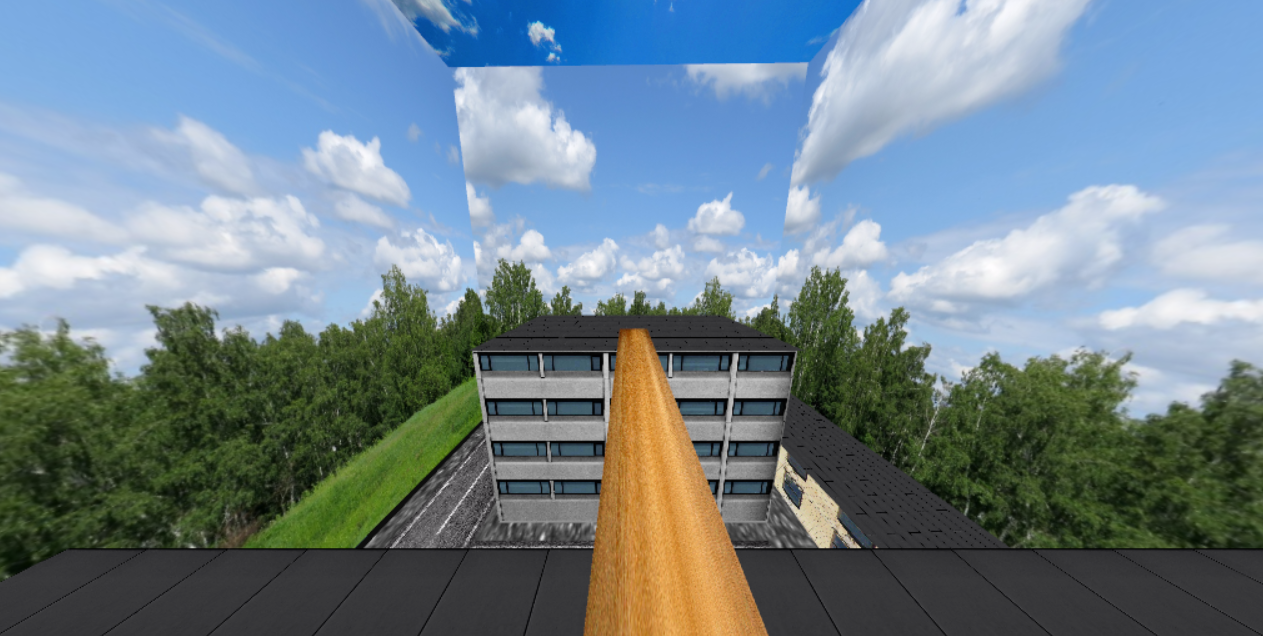
\includegraphics[scale=0.202]{vueBasiqueTextures.png}
   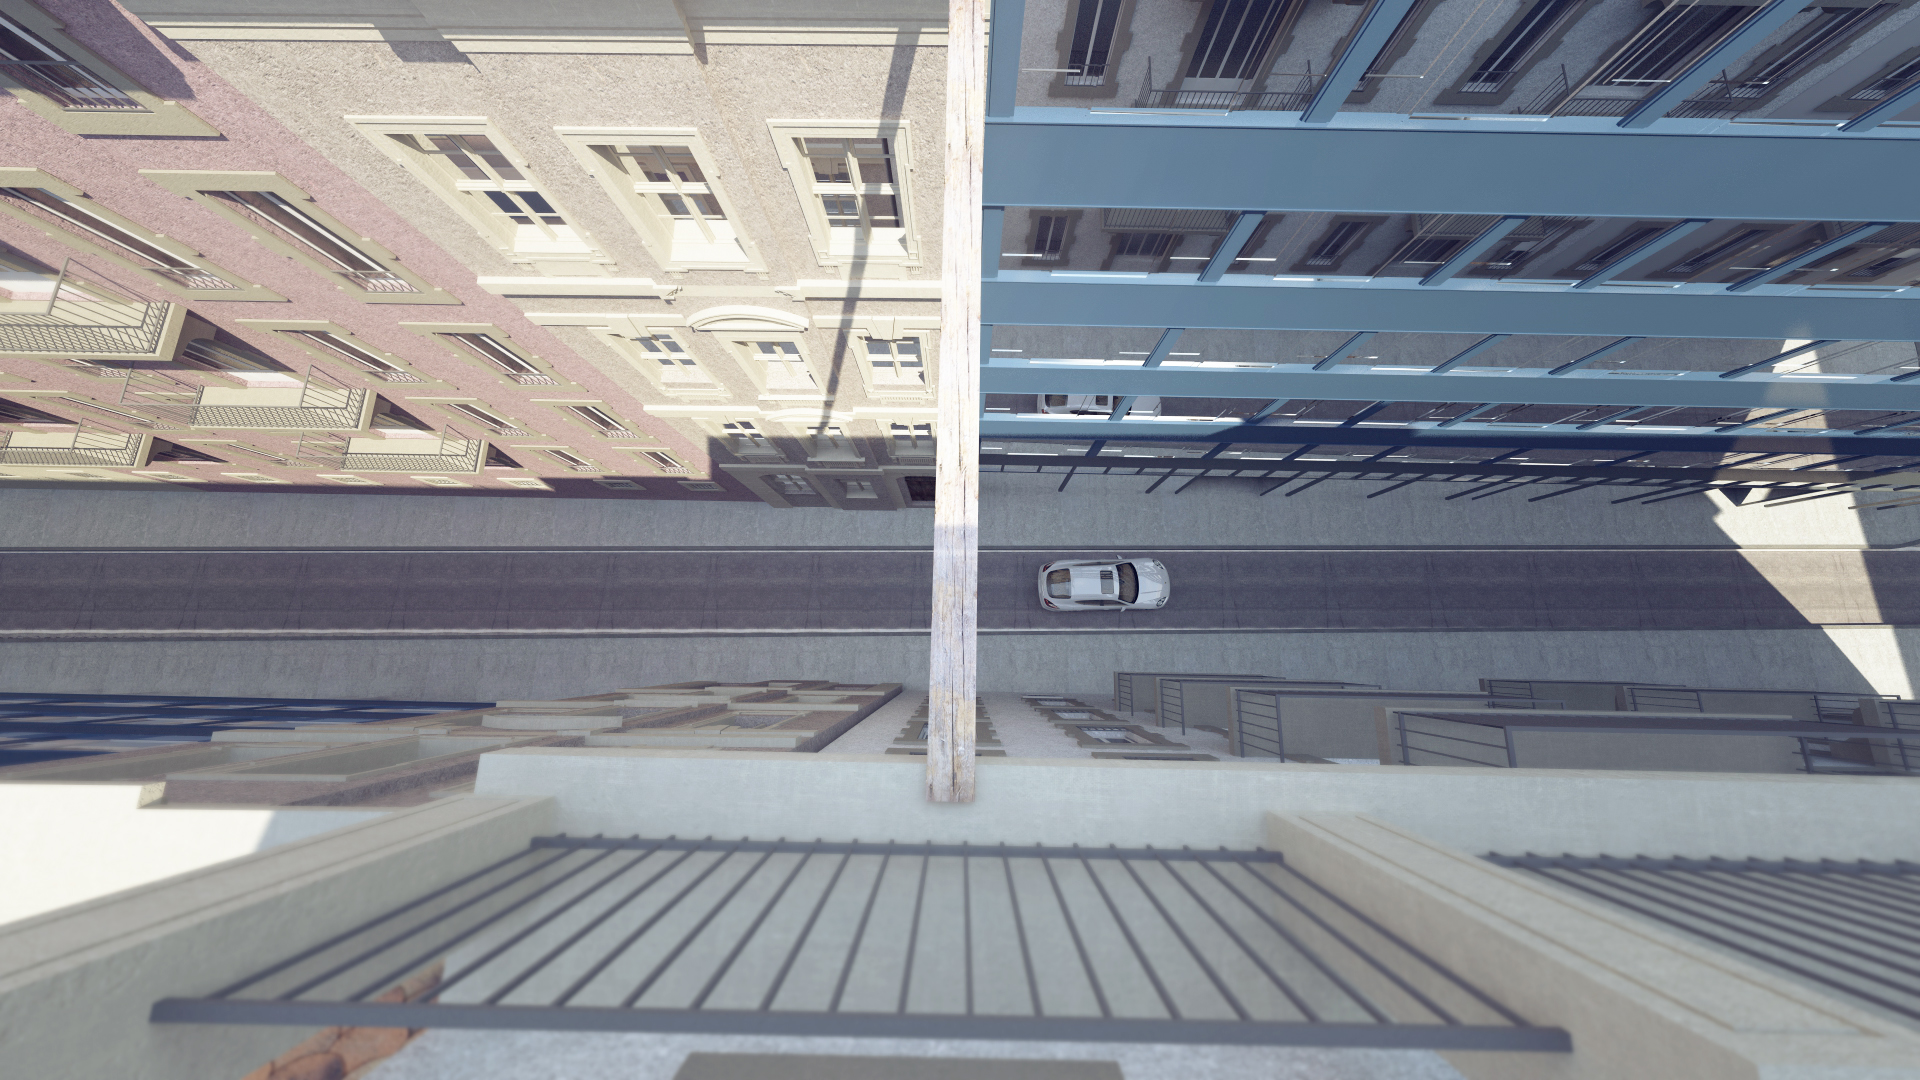
\includegraphics[scale=0.09]{Vue_planche2_ok.jpg}
   \caption{\label{textures} Illustrations vue virtuelle avec textures}
\end{figure}

%%%%%%%%%%%%%%%%%%%%%%%%%%%%%%%%%%%%%%%%%%%%%%%%%%%%%%%%%%%%%%%%%%%%%%%%%%%%%%%%%%%%%%%%%%%%%%%%%%%%%%%%%%%%%%%%%%%%%%%%%%%%
\pagebreak
\section{Animations sur la réalité virtuelle} \label{animation}
La prise en charge des différentes animations de la réalité virtuelle est locale au périphérique exécutant l'application.

\subsection*{Placement de la caméra}  \label{camera}
Le placement de la caméra s'effectue avec la balise \texttt{<viewpoint>}, en utilisant son attribut \texttt{position} correspondant au vecteur de position. Avec cette balise, il est possible de placer la caméra à la position de la tête.\\
Sur la vue du \textsf{smartphone}, la caméra se place en même temps que la tête avance. Il faut pour cela mettre à jour cet attribut à chaque changement.\\
Sur la vue de l'ordinateur, la caméra peut se déplacer comme sur la vue du \textsf{smartphone} ou être à un point fixe derrière la personne. Ces deux points de vues donnent une perspective différente.\\

A noter que la balise \texttt{<viewpoint>} est englobée par une balise \texttt{<transform>} qui permet d'effectuer une rotation suivi d'une translation. La rotation permet à la caméra de se placer perpendiculairement aux immeubles. La translation déplace la caméra sur un seul axe sans avoir à changer la position initiale de la caméra. \\ 

L'illustration~\ref{positionsCamera} ci-dessous montre la position de la caméra sur le \textsf{smartphone} et les deux positions de caméra possibles sur l'écran standard.
\begin{figure}[H]
\centering
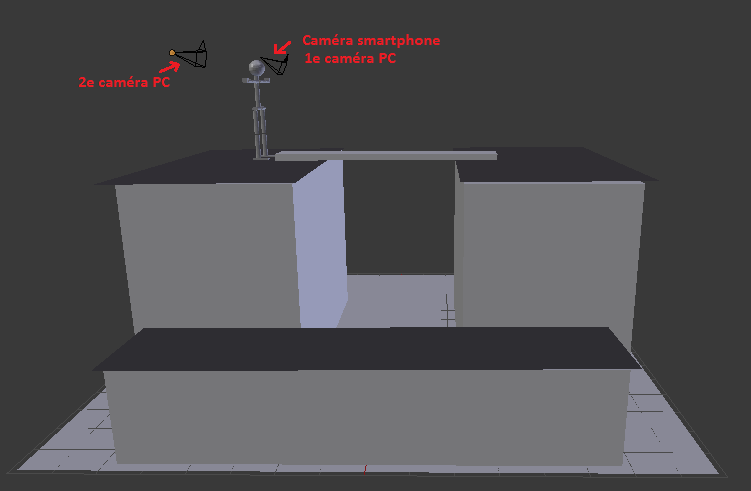
\includegraphics[scale=0.5]{positionCamera.png}
\caption{\label{positionsCamera} Illustrations des positions possibles de la caméra}
\end{figure}

\pagebreak
\subsection*{Orientation de la tête}  \label{orientation}
L'orientation de la tête s'effectue en utilisant l'accéléromètre du \textsf{smartphone}. L'accéléromètre mesure la force d'accélération appliquée au \textsf{smartphone} sur les axes x, y et z (force de gravitation). Il est utilisé pour détecter les mouvements. L'illustration~\ref{accelerometre} ci-dessous illustre les axes de l'accéléromètre.
\begin{figure}[H]
\centering
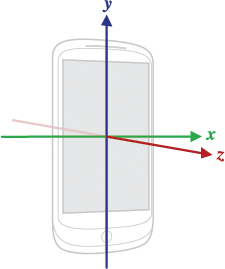
\includegraphics[angle=90,origin=c,scale=0.4]{accelerometre.png}
\caption{\label{accelerometre} Illustration des axes de l'accéléromètre}
\end{figure} 

La rotation de la vue en fonction des mouvements de la tête s'effectue en plusieurs étapes :

\begin{enumerate}
\item récupérer la rotation du \textsf{smartphone} dans un quaternion en utilisant des paramètres mis à disposition par \textit{X3DOM}
\begin{lstlisting}
var q0 = x3dom.fields.Quaternion.axisAngle(new x3dom.fields.SFVec3f(0,0,1),-deg2rad(window.orientation));		       
\end{lstlisting}

\item créer un quaternion avec les valeurs de l'accéléromètre
\begin{lstlisting}
var q = new x3dom.fields.Quaternion();
q.setFromEulerYXZ(deg2rad(MYAPP.deviceOrientation.beta), deg2rad(MYAPP.deviceOrientation.alpha), -deg2rad(MYAPP.deviceOrientation.gamma));
\end{lstlisting}

\item créer un quaternion afin de tourner la caméra car l'orientation captée par le \textsf{smartphone} pointe vers le haut
\begin{lstlisting}
var q1 = new x3dom.fields.Quaternion.axisAngle(new x3dom.fields.SFVec3f(1,0,0),-Math.PI/2); 
\end{lstlisting}

\item multiplier le quaternion des valeurs de l'accéléromètre avec les deux autres quaternions
\begin{lstlisting}
q = q.multiply(q1);
q = q.multiply(q0);
\end{lstlisting}

\item transformer le quaternion des valeurs de l'accéléromètre en un vecteur de position avec un angle de rotation
\begin{lstlisting}
var orientation = q.toAxisAngle();
\end{lstlisting}

\item appliquer les valeurs de accéléromètre à l'attribut \texttt{orientation} de la caméra 
\begin{lstlisting}
MYAPP.viewpoint.setAttribute("orientation", orientation[0].x + " " + orientation[0].y + " " + orientation[0].z + " " + orientation[1]);
\end{lstlisting}
\end{enumerate}

\subsection*{Avancement sur la planche}  \label{avancement}
L'avancement du personnage sur la planche virtuelle s'est effectué en deux temps en modifiant les balises \textit{X3DOM} :\\


\begin{enumerate}
\item \textbf{Simulation du déplacement du personnage sur la planche : } \\
Pour mettre en place ce déplacement fictif, une récursivité a été implémentée. Toutes les secondes, la distance définie diminue. Le personnage est alors déplacé et la vue suit ce déplacement. Cette récursion tourne en boucle parce que lorsque la distance est égale à la distance minimum définie, les valeurs sont réinitialisées.

\begin{lstlisting}[language=JavaScript]	
function moveFictif(){
	timer--;
	character.attr("translation", timer +' 20 2');
	vp.attr("position",'0 10 '+ timer);
	vp.attr("centerOfRotation", '0 10 '+ timer);

	if (timer <= -MAX_Z)
		timer = MAX_Z;
	
	sleep(1);
	moveFictif();
}
\end{lstlisting}


\item \textbf{Avancement du personnage en fonction du \textit{Kinect} et selon la positon de la tête :} \\
Au commencement de la simulation, la personne se place face au \textit{Kinect} à environ 4 mètres de distance. Puis elle commence à avancer sur la planche en portant les lunettes. La vue affichée sur le \textsf{smartphone} sera adaptée en fonction de ces déplacements. Les membres peuvent être vus lors de la simulation. Pendant le déplacement, une vérification est effectuée afin de savoir si la personne a "chuté".

\begin{lstlisting}[language=JavaScript]	
function move(){
	if (position.head != undefined)
		if ((position.head.z > 3.90 & !start) ){
			start = true; 
			document.getElementById('music').play();
		}else if (position.head.z < 0.70 & start)
			start = false;

		if (start){
			// only the all armature move, the animation of the member is not handle here
			vp.attr("position", (parseFloat(position.head.x) -0.2) + " " + (parseFloat(position.head.y) -0.2)+ " " + (parseFloat(position.head.z) -0.2));
			vp.attr("centerOfRotation", (parseFloat(position.head.x) -0.2) + " " + (parseFloat(position.head.y) -0.2)+ " " + (parseFloat(position.head.z) -0.2));
			$("#armature").attr("translation",  (parseFloat(position.head.z) - 4.0) + " 7.3 0");
			$("#camera").attr("translation", (parseFloat(position.head.z) - 4.0) + " 8 " + (parseFloat(position.head.x) -0.2) );
			checkBoundries();

		}
	}
\end{lstlisting}
\end{enumerate}

\subsection*{Animation du personnage} \label{animationPersonnage}
L'animation du personnage était un aspect important du projet car on voulait que la personne puisse voir ses membres lors de la simulation. Au cours du développement, l'animation du personnage a posé quelques problèmes (voir le chapitre~\ref{problemes}). Comme mentionné dans la section~\ref{traitement}), l'animation du personnage a été effectuée en suivant les étapes : \\

\begin{enumerate}

\item \textbf{Distance en deux dimensions entre des points $A=(A_x,A_y)$ et $B=(B_x,B_y)$ :}
\begin{equation}
AB = \sqrt{(B_x - A_x)^2 + (B_y - A_y)^2}
\end{equation}

\item \textbf{Angle entre 2 points A et B : }
L'angle est calculé selon le triangle rectangle suivant : 

\begin{figure}[H]
\centering
	\includegraphics[scale=0.7]{Triangle.jpg}
	\caption{\label{triangle} Triangle rectangle utilisé pour le calcul de l'angle $a$}
\end{figure}

\begin{equation}
a = \mathrm{atan2}((B_y - A_y), (A_x - B_x))
\end{equation}
(La description de atan2 se trouve à la section~\ref{atan2}).\\

\item  \textbf{Positionnement du membre entre les points A et B :} une simple translation du cylindre correspondant à l'id à la position de l'articulation A. Le cylindre est positionné en fonction du point d'origine A et du point de fin B.

\begin{lstlisting}
function positionning(id, pos){
	$("#"+id).attr("translation", (pos.x) + " " +  (pos.y -0.5) + " " + pos.z);
}
\end{lstlisting}
\pagebreak
\item  \textbf{Adaptation de la taille du membre : } un \textsf{scaling} appliqué en x, correspondant à la longueur, au bon cylindre utilisant la distance calculée auparavant entre les 2 points~A~et~B.
\begin{lstlisting}
function scaling(id, distance, old){
	var distance = distance.toFixed(2);
	if (distance != old){
		$("#"+id).attr("scale", distance  +" "+ DIV_DISTANCE + " " + DIV_DISTANCE );
		old = distance;
	}
	return old;
}
\end{lstlisting}

\item \textbf{Rotation du membre : } une rotation est appliquée en z en utilisant l'angle calculé auparavant.
\begin{lstlisting}
function anime(id, angle, old){
	var angle = angle.toFixed(2);
	if (angle != old){
		$("#"+id).attr("rotation", "0 0 1 " + angle);
		old = angle;
	}
}
\end{lstlisting}
\end{enumerate}

A noter qu'un \textsf{objet json} a été mis en place contenant pour chaque membre relié : 
\begin{itemize}
\item un id correspondant à l'identification du cylindre 3D 
\item un membre A correspondant au membre de départ
\item un membre B correspondant au membre d'arrivé 
\end{itemize}

\begin{figure}[H]
\centering
\includegraphics[scale=0.7]{jsonRelie.jpg}
\caption{\label{jsonrecu} Illustration de l'objet json des articulations reliées}
\end{figure}

A noter également que l'ordre des membres A et B est important pour l'animation. Car s'ils sont inversés l'animation se fera dans l'autre sens. Par exemple, si le membre A est le coude gauche et le membre B l'épaule gauche, le cylindre correspondant au bras sera placé aux positions du coude. Cela affecterait également la rotation du membre car le point de départ serait le coude.

\subsection*{Atan2} \label{atan2}
Atan2 est une variante de la fonction arc tangente prenant en paramètres deux valeurs. Pour tout paramètre réel non nul, atan2 est l'angle en radians entre la partie positive de l'axe des x d'un plan et le point de ce plan aux coordonnées passées en paramètres. L'angle donné est positif pour les angles dans le sens trigonométrique (sens anti-horaire) et négatif dans l'autre sens (pour plus d'information sur atan2 \cite{atan2}).
\pagebreak
\subsubsection{Définition et illustrations}
Pour $y \ne  \ 0$: \\
\begin{figure}[H]
	\centering
	\includegraphics[scale=0.6]{atan2Y0.png} 
\end{figure}
où $\varphi $ \ est l'angle compris entre [0, $\Pi$ /2] de façon à ce que $\mathrm{tan}(\varphi) = |y/x|$ et sgn est la fonction signe. \\

Et: 
\begin{figure}[H]
	\centering
	\includegraphics[scale=0.75]{atan22.png} 
\end{figure}

\begin{figure}[H]
	\centering
	\includegraphics[scale=0.5]{atan2Circle.png} 
	\caption{\label{atan2circle} Illustration du cercle trigonométrique des valeurs de atan2}
\end{figure}
Le cercle ci-dessus illustre les valeurs, en radians, de atan2. Les angles sont inscris en bleu et les points sont inscris à l'extérieur du cercle. 


\subsection*{Effet sonore}  \label{sonore}
L'ajout d'un effet sonore lors de la simulation semblait indispensable afin de permettre à l'utilisateur mieux s'intégrer dans sa simulation. Cet effet sonore est un enregistrement du bruit ambiant à la fenêtre. Il a été ajouté en HTML5 et est activé, en \textsf{JavaScript}, lorsque la personne se trouve au bord de la planche.

\subsection*{Chute et recommencement}  \label{chute}
Une animation de "chute" a été implémentée. Lorsque la personne "chute", c'est-à-dire qu'elle a les deux pieds en dehors de la planche. La personne voit la vue descendre au fur et à mesure de la "chute". La désactivation cette option est possible si la personne ne le supporte pas. \\

La possibilité de recommencer la simulation est également important afin d'éviter de devoir recharger la page à chaque fois. Lorsque la personne "chute" ou qu'elle arrive de l'autre côté de la planche, la vue de départ revient après quelques secondes et la personne peut recommencer.
\chapter{Problèmes rencontrés} \label{problemes}
Comme dans chaque projet, un ensemble de problèmes se sont produits. Dans ce chapitre se trouve la description de chaque problème majeur rencontré.

\section*{Utilisation du Kinect en passant par NodeJS}  \label{probNodeKinect}
A la fin du projet de semestre, un projet \textit{GitHub} Node Kinect \cite{NodeKinect} a été trouvé. Il permet de capturer les données du \textit{Kinect} directement avec \textit{NodeJS}, donc de ne pas utiliser \textit{Visual Studio} et d'avoir un projet entièrement en \textsf{JavaScript}. \\ 

Le projet \textit{Node Kinect} utilise les outils suivants :
\begin{itemize}
\item La librairie \textit{Libusb} est une libraire C, open source, qui donne accès aux périphériques USB sur beaucoup de systèmes d'exploitation (pour plus d'information voir \cite{libusb}).\\ 
Elle permet de communiquer avec le \textit{Kinect}. 
\item Le driver \textit{Libfreenect} est un driver implémenté par \textit{OpenKinect}. \textit{OpenKinect} est une communauté open source de personnes qui veulent faire fonctionner le \textit{Kinect} avec d'autres systèmes d'exploitation que Windows (pour plus d'informations sur \textit{Libfreenect}~\cite{libfreenect} ou sur OpenKinect~\cite{OpenKinect}).  \\
Ce driver permet de capturer les données du \textit{Kinect} et donc de substituer le \textit{Kinect SDK}. \\

\end{itemize}

Lors de l'installation de \textit{Libfreenect} et de l'installation des logiciels nécessaires à son fonctionnement, des erreurs apparaissaient car plusieurs logiciels ou librairies manquaient. Après plus d'une semaine bloquée sur cette installation et donc dans l'incapacité de commencer à utiliser le \textit{Kinect}, l'utilisation du projet \textit{Node Kinect} a été abandonnée. Finalement, la gestion du \textit{Kinect} dans \textit{Virtual-Vertigo} s'est faite avec le \textit{Kinect SDK 1.8, Visual Studio et C\#} \. L'envoi des données capturées passe par un serveur Web.

%%%%%%%%%%%%%%%%%%%%%%%%%%%%%%%%%%%%%%%%%%%%%%%%%%%%%%%%%%%%%%%%%%%%%%%%%%%%%%%%%%%%%%%%%%%%%%%%%%%%%%%%%%%%%%%%%%%%%%%%%%%
\section*{Utilisation KinectHTML5 sur un site sécurisé}  \label{probKinectHTML5}
Toujours durant le travail de semestre, le projet \textit{Visual Studio KinectHTML5} \cite{KinectHTML5} a été trouvé. Ce projet permet de capturer des données du \textit{Kinect} et de les envoyer via les \textit{WebSockets} à un client HTML5. Il a été choisi car il correspondait aux besoins du projet \textit{Virtual-Vertigo}. Le projet \textit{KinectHTML5} est constitué de deux parties :
\begin{enumerate}
\item un projet client dans lequel se trouve la page HTML5 et les scripts nécessaires à la connexion aux \textit{WebSockets}, à la récupération des données du \textit{Kinect} et l'affichage des informations captées sur un canvas;
\item un projet serveur sur lequel s'exécute le serveur \textit{WebSocket} et où se font la capture et l'envoi des données.\\

\end{enumerate}

En utilisant ce projet localement tout fonctionnait parfaitement. Cependant, lors de l'intégration de ce projet au serveur d'hébergement, ça ne fonctionnait plus. En effet, \textit{KinectHTML5} utilise des \textit{WebSockets} tandis que le serveur d'hébergement utilise HTTPS. Pour que le projet fonctionne, il fallait l'adapter pour utiliser des \textit{WebSockets} sécurisés. Mais les \textit{WebSockets} sécurisés nécessitent un certificat. Celui-ci a alors été créé mais il a été impossible de l'ajouter au serveur d'hébergement. \\

La solution a été d'utiliser un \textit{serveur NodeJS} avec \textit{Socket.io} servant de pont entre les clients HTML et le \textit{Kinect}. Après quelques recherches, le \textit{projet Visual Studio SocketIOC\# Client} a été trouvé. Il permet à un programme C\# de se connecter à un \textit{serveur NodeJS} utilisant \textit{Socket.io} (pour plus d'informations sur le projet \textit{SocketIOC\#} voir \cite{SocketIOCSharp} ou sur \textit{Socket.io} \cite{SocketIO}).

%%%%%%%%%%%%%%%%%%%%%%%%%%%%%%%%%%%%%%%%%%%%%%%%%%%%%%%%%%%%%%%%%%%%%%%%%%%%%%%%%%%%%%%%%%%%%%%%%%%%%%%%%%%%%%%%%%%%%%%%%%%

\section*{Animation du personnage - mapping squelette kinect et squelette blender}  \label{probSquelette}

Lorsque le personnage virtuel 3D a été créé avec \textit{MakeHuman}, un squelette a été ajouté au personnage afin de pouvoir l'animer. Pour une animation la plus réaliste possible, l'idée de mapper le squelette du \textit{Kinect} et le squelette présent dans le personnage 3D est apparu. Cependant, après quelques recherches et tests, il était impossible de mapper les deux squelettes. En effet, lorsque le personnage est exporté en format X3D avec \textit{Blender}, le personnage devient rigide. Il est impossible d'accéder à chaque membre du squelette dans le personnage.\\

La solution mise en place favorise l'animation des membres au dépend du réalisme du personnage 3D. Le squelette de la personne a été reconstruit en 3D directement sur \textit{X3DOM}. En utilisant les données reçues, cela a permis d'animer les membres du personnage. L'animation des membres a été effectuée en calculant l'angle entre les articulations reliées. Cet angle permet de savoir comment effectuer la rotation du membre.

%%%%%%%%%%%%%%%%%%%%%%%%%%%%%%%%%%%%%%%%%%%%%%%%%%%%%%%%%%%%%%%%%%%%%%%%%%%%%%%%%%%%%%%%%%%%%%%%%%%%%%%%%%%%%%%%%%%%%%%%%%%

\section*{Animation du personnage - calcul de l'angle}  \label{probAngle}

Comme mentionné dans la section précédente, un angle a été calculé entre les articulations reliées. L'angle a été calculé, considérant chaque articulation comme un point dans l'espace. Le calcul de l'angle entre deux points est impossible. Nous avons donc calculé un troisième point avec les coordonnées des deux autres points afin de créer un triangle rectangle.\\

\begin{figure}[H]
	\centering
   		\includegraphics[scale=0.7]{Triangle.jpg}
   \caption{\label{triangle rectangle} Illustration du triangle rectangle}
\end{figure}
Sur l'illustration~\ref{triangle rectangle}, les deux points correspondant aux articulations sont en rouge, le troisième point étant en vert (une combinaison des deux autres points). En traçant les droites entre chaque point, il est possible de créer un triangle rectangle. Il permet d'utiliser les formules trigonométriques, telles que le calcul de la distance entre deux points et le calcul des angles dans un triangle rectangle. \\

Les formules de calcul de distance entre deux points appliquées sur ce triangle sont les suivantes : \\
\begin{equation}
AC = \sqrt{(B_x - A_x)^2 + (A_y - A_y)^2}
\end{equation}
\begin{equation}
BC = \sqrt{(B_x - B_x)^2 + (A_y - B_y)^2} 
\end{equation}
\begin{equation}
AB = \sqrt{(B_x - A_x)^2 + (B_y - A_y)^2} 
\end{equation}
où $A=(A_x,A_y)$, $B=(B_x,B_y)$ et $C=(B_x,A_y)$

Les formules de calcul de l'angle appliquées sur ce triangle sont les suivantes : \\
\begin{equation}
b = \mathrm{acos}{(BC/AB)}
\end{equation}
\begin{equation}
a = \mathrm{asin}{(AC/AB)}
\end{equation}

Cependant, en effectuant l'implémentation de ces calculs, ceux-ci n'étaient pas assez précis et trop lents, parce que la disposition des articulations n'a pas été prise en compte. Les membres ne se déplaçaient pas comme ils le devaient. Finalement, le calcul de l'angle a été effectué en utilisant la fonction atan2 décrite à la section~\ref{atan2}. L'utilisation de cette fonction a rendu l'animation des membres plus précise et dynamique.

%%%%%%%%%%%%%%%%%%%%%%%%%%%%%%%%%%%%%%%%%%%%%%%%%%%%%%%%%%%%%%%%%%%%%%%%%%%%%%%%%%%%%%%%%%%%%%%%%%%%%%%%%%%%%%%%%%%%%%%%%%%
\pagebreak
\section*{Des données captées à la réalité}  \label{probRealite}
Lors du développement, nous avons réalisé que le \textit{Kinect} ne transmettait pas les données qu'il capte en fonction de la réalité. En effet, le \textit{Kinect} transmettait les données en fonction de son angle de vue conique. En effet l'utilisation d'un objet \texttt{CoordinateMapper} ne renvoyait pas les dimensions réelles de la personne. Pour remédier à ce problème, des mesures ont été effectuées sur un rectangle délimité :
\begin{figure}[H]
	\centering
		\includegraphics[scale=1]{RectangleMesures.png}
	\caption{\label{rectangleMesures} Rectangle créé sur le sol afin d'effectuer les mesures}
\end{figure}

Ces mesures ont été réalisées tous les 40 centimètres au centre du rectangle. Les points de repères suivants ont été définis :
\begin{itemize}
\item pour la distance entre deux articulations, le centre des épaules et la colonne vertébrale
\item pour l'axe x, la main posée sur une table à 3 endroits différents afin ne pas fausser les mesures entre chaque déplacement
\item pour z, les 2 pieds placés après les lignes tracées au sol \\

\end{itemize}

Voici les résultats obtenus : 
\begin{center}
	\begin{tabular}{|*{6}{c|}}
	\hline
		\textbf{Z} & \textbf{Distance} & \textbf{Z Kinect} & \textbf{Coin gauche} & \textbf{Milieu} & \textbf{Coin droit}  \\ \hline
		0.80 & 169 & 0.85 & 44 & 276 & 475\\ \hline
		1.20 & 147 & 1.25 & 72 & 271 & 447\\ \hline
		1.60 & 112 & 1.65 & 105 & 294 & 420\\ \hline
		2.00 & 92 & 2.05 & 134 & 274 & 397\\ \hline
		2.40 & 79 & 2.46 & 158 & 261 & 362\\ \hline
		2.80 & 69 & 2.86 & 160 & 257 & 357\\ \hline
		3.20 & 60 & 3.24 & 177 & 270 & 343\\ \hline
		3.60 & 54 & 3.65 & 183 & 257 & 334\\ \hline
		3.85 & 50 & 3.90 & 187 & 302 & 290\\ \hline
	\end{tabular}
\end{center}

En analysant ce tableau, les valeurs en z correspondent à la réalité moyennant un décalage de 0.5 cm. Cependant les valeurs mesurées en x ne correspondent pas et n'aide pas à trouver une formule pouvant être appliquée. Un graphique peut être tracé avec les valeurs des distances entre le centre des épaules et la colonne vertébrale: \\

\begin{figure}[H]
	\centering
		\includegraphics[scale=0.7]{evolutionDistance.png}
	\caption{\label{evolutionDistance} Évolution de la distance entre les épaules et la colonne}
\end{figure}

Finalement, le problème a été corrigé sans utiliser ces mesures. Le programme capturant les données du \textit{Kinect} a complètement été réécrit afin de capturer les données de manière absolue. En utilisant cette méthode, les valeurs en x et y capturées sont en mètres et correspondent à la réalité. 

%%%%%%%%%%%%%%%%%%%%%%%%%%%%%%%%%%%%%%%%%%%%%%%%%%%%%%%%%%%%%%%%%%%%%%%%%%%%%%%%%%%%%%%%%%%%%%%%%%%%%%%%%%%%%%%%%%%%%%%%%%%

\section*{Taille de la scène finale}  \label{taille}

Comme mentionné dans le chapitre~\ref{vertigo}, une des vues finales du projet a été modélisée par \textsc{M. Benjamin Dupond-Roy}. Malheureusement, la première vue modélisée était trop détaillée et le fichier correspondant trop grand ce qui empêchait le smartphone de l'afficher. Le chargement sur PC était également ralenti. \textsc{M. Benjamin Dupond-Roy} a donc modélisé une vue plus petite afin qu'elle s'affiche correctement sur le \textsf{smartphone} et ne ralentisse pas le PC. \\
Ci-dessous un tableau illustrant la taille des fichiers X3D générés par \textit{Blender} et utilisés sur \textit{X3DOM} : 

\begin{center}
	\begin{tabular}{| l | c |}
	\hline
	\textbf{Scènes} & \textbf{Taille fichier X3D en Ko} \\ \hline
	Scène basique contenant les textures & 28 Ko \\\hline
	Première scène modélisée par \textsc{M. Benjamin Dupond-Roy} sans textures & 37 505 Ko \\ \hline
	Deuxième scène modélisée par \textsc{M. Benjamin Dupond-Roy} sans textures & 11 396 Ko \\ \hline
	\end{tabular}
	\captionof{table}{\label{tailles} Tableau illustrant les tailles des scènes modélisées exportées en X3D}
\end{center}

Comme vous pouvez le voir, la scène basique est très petite. Cela permet d'être chargée rapide et d'avoir une simulation fluide. La deuxième scène modélisée par \textsc{M. Benjamin Dupond-Roy} est trois fois plus petite que la première. Elle s'affiche correctement sur le \textsf{smartphone} et le PC mais n'est pas aussi fluide que la scène basique.

%%%%%%%%%%%%%%%%%%%%%%%%%%%%%%%%%%%%%%%%%%%%%%%%%%%%%%%%%%%%%%%%%%%%%%%%%%%%%%%%%%%%%%%%%%%%%%%%%%%%%%%%%%%%%%%%%%%%%%%%%%%
\section*{Calibrage de la vue sur le smartphone}  \label{calibrage}

Lorsque la personne se trouve au bord de la planche  prête à commencer la simulation, le \textsf{smartphone} prend en charge l'orientation de la vue en utilisant son accéléromètre. Parfois, lorsqu'il prend la main, le \textsf{smartphone} décale la vue. Elle n'est plus alignée sur la planche ce qui fait que la personne sur la planche se décale.\\

Deux solutions pourraient être implémentées : 
\begin{enumerate}
\item utiliser l'aimant des \textit{Google CardBoard} pour interagir avec le \textsf{smartphone} afin de déclencher un événement de calibrage de la vue;
\item utiliser un signe de la main que le \textit{Kinect v1} reconnait afin de signaler que le calibrage doit s'effectuer.
\end{enumerate} 
\chapter{Conclusion}

%%%%%%%%%%%%%%%%%%%%%%%%%%%%%%%%%%%%%%%%%%%%%%%%%%%%%%%%%%%%%%%%%%%%%%%%%%%%%%%%%%%%%%%%%%%%%%%%%%%%%%%%%%%%%%%%%%%%%%%%%%%

\section{Bilan}
L'objectif du projet \textit{Virtual-Vertigo} était de réaliser un exercice pour combattre la peur du vide en utilisant des \textit{Google CardBoard} pour visualiser un déplacement dans un monde virtuel. Celui-ci est constitué d'une planche reliant deux immeubles. La personne doit traverser cette planche pour atteindre l'immeuble d'en face sans "chuter". \\

Les éléments suivants ont été mis en place afin d'avoir une simulation opérationnelle :

\begin{itemize}
\item La modélisation de deux scènes virtuelles 3D constituées d'une planche reliant deux immeubles. \\
Cette scène est affichée sur une page Web en utilisant le \textit{Framework X3DOM} permettant d'afficher des scènes 3D. Les scènes ont été modélisées en utilisant des logiciels 3D \textit{Blender et Cinema4D}.
\begin{figure}[H]
\centering
\includegraphics[scale=0.17]{VueBasique2.png}
\includegraphics[scale=0.07]{Vue_balcon2_ok.jpg}
\caption{\label{vue} Illustration des scènes virtuelles 3D créées}
\end{figure}

\item La mise en place du \textit{serveur Web Virtual-Vertigo} servant de pont entre le \textit{Kinect version 1} et les clients HTML (le \textsf{smartphone} et le PC). \\
Ce serveur utilise \textit{NodeJS} avec les \textit{modules ExpressJS et Socket.io}.

\item La création d'un \textit{projet Visual Studio} pour le \textit{Kinect} pour la capture des données de positions (articulations du squelette et orientations des mains) et de les transmettre au \textit{serveur Web Virtual-Vertigo} en utilisant SocketIOC\#.
\begin{figure}[H]
\centering
\includegraphics[scale=0.5]{squelette.jpg}
\caption{Illustration des articulations du squelette capturées par le \textit{Kinect v1}}
\end{figure}

\item La création d'un personnage 3D réaliste avec \textit{MakeHuman}.\\
Ce personnage n'est pas utilisé dans la version finale car il est devenu rigide lors de l'exportation en X3D depuis \textit{Blender}.
\begin{figure}[H]
\centering
\includegraphics[scale=0.4]{PersonnageRealiste.png}
\caption{Illustration du personnage réaliste créé}
\end{figure}

\item La création d'un client HTML pour le \textsf{smartphone} contenant une vue stéréoscopique de la réalité virtuelle utilisant \textit{X3DOM}. \\ Un problème avec le positionnement des textures visible sur la figure~\ref{vueSmartphone} persiste.
\begin{figure}[H]
\centering
\includegraphics[scale=0.15]{VueSmartphone.png}
\caption{\label{vueSmartphone} Illustration de la vue stéréoscopique sur le \textsf{smartphone}}
\end{figure}

\item La création d'un client HTML pour le PC pour afficher la simulation sur un écran standard toujours avec \textit{X3DOM}.
\item La construction d'un squelette 3D dans la réalité virtuelle afin de l'animer. \\
Des sphères sont placées sur les articulations et des cylindres relient les articulations voisines.
\item Le déplacement (en \textsf{JavaScript}) de la personne sur la planche dans la réalité virtuelle en fonction de la position de la tête capturée par le \textit{Kinect version 1}.
\begin{figure}[H]
\centering
\includegraphics[scale=0.15]{Deplacement.png}
\caption{\label{Deplacement} Illustration du déplacement du squelette 3D dans la réalité virtuelle}
\end{figure}

\item L'animation des membres du squelette 3D en fonction des données capturée par le \textit{Kinect version 1}. \\
Cela nécessitait de positionner et calculer l'angle entre deux articulations voisines du squelette.
\item L'adaptation de la scène virtuelle en fonction de l'orientation de la tête. \\
Cette orientation est détectée via les accéléromètres du \textsf{smartphone}.
\item L'ajout d'effets afin de rendre la simulation plus réaliste : \\
\begin{itemize}
\item une planche réelle sur le sol.
\item un bruit ambiant en utilisant un casque sans fil.
\item une animation de "chute" lorsque l'utilisateur n'a plus les pieds sur la planche. \\
La simulation recommence après une "chute" ou lorsque l'utilisateur est arrivé à l'extrémité de la planche.
\end{itemize}
\end{itemize}

La figure~\ref{simulation} montre à gauche un camarade de diplôme, \textsc{M. Vasco Marques}, effectuant la simulation du projet et à droite la vue affichée sur les \textit{Google CardBord} lors de sa simulation.
\begin{figure}[H]
\centering
	\includegraphics[scale=0.03]{vueReelle1.jpg}
	\includegraphics[scale=0.2]{vueBasiqueTextures.png}
\caption{\label{simulation} Simulation de Virtual-Vertigo}
\end{figure}

A la fin de ce travail de Bachelor, une simulation complète est opérationnelle. Il est possible de porter les \textit{Google CardBoard} et de faire la simulation en ayant une planche posée sur le sol et un casque \textsf{bluetooth} diffusant un bruit ambiant enregistré. Cependant quelques problèmes n'affectant pas la simulation persistent: 
\begin{enumerate}
\item le décalage de la vue lorsque le \textsf{smartphone} prend le relais pour l'orientation de la vue en fonction de la tête;
\item le positionnement non optimal des textures dans la vue affichée sur le \textsf{smartphone};
\item la visualisation  non optimale des membres qui parfois ne s'affichent pas alors que la personne tient ses mains bien devant elle (ils paraissent plus petits en virtuel que dans la réalité).
\end{enumerate}

%%%%%%%%%%%%%%%%%%%%%%%%%%%%%%%%%%%%%%%%%%%%%%%%%%%%%%%%%%%%%%%%%%%%%%%%%%%%%%%%%%%%%%%%%%%%%%%%%%%%%%%%%%%%%%%%%%%%%%%%%%%

\section{Améliorations}
Quelques améliorations possibles pour ce projet sont les suivantes :
\begin{itemize}
\item corriger les problèmes persistants 
\item ajouter le reste des effets de réalisme (la montre connectée et le ventilateur)
\item utiliser la \textit{Kinect v2} afin d'avoir plus de précisions sur l'orientation des mains
\item utiliser le \textsf{smartphone} pour lancer l'effet sonore au lieu du casque sans fil
\item trouver d'autres effets de réalisme pour augmenter l'immersion de la personne 
\item améliorer les \textit{Google CardBoard} afin de les rendre plus esthétiques et plus agréable à porter
\item étudier la possibilité d'un composant disponible sur le \textsf{smartphone} en remplacement de la \textit{Kinect}
\end{itemize} 

\section{Perspectives}
Afin de pouvoir vraiment utiliser le projet \textit{Virtual-Vertigo} dans un contexte médical, il faudrait contacter un psychologue ou un spécialiste pour évaluer le projet. Cette évaluation permettrait de savoir si l'approche choisie pour ce projet est vraiment utile pour aider les personnes ayant le vertige. En cas de succès auprès d'un spécialiste, le projet pourrait être lancé avec une \textsf{startup} et serait distribué dans la médecine thérapeutique. Une autre possibilité de vente serait envisageable. En effet, l'armée ou les services de pompiers pourraient être intéressés par des variantes de \textit{Virtual-Vertigo}. Celles-ci pourraient leur être utile afin de tester ou entraîner leurs nouvelles recrues dans un environnement virtuel similaire à celui de \textit{Virtual-Vertigo}. 


\appendix
\addcontentsline{toc}{chapter}{Annexes}
\chapter{Glossaire} \label{glossaire}

\subsubsection*{Réalité virtuelle}
Simulation informatique interactive immersive, en temps réel pouvant être visuelle, sonore ou haptique d'environnements réels ou imaginaires.

\subsubsection*{Google CardBoard}
Casque de réalité virtuelle en carton contenant des lentilles et un smartphone.

\subsubsection*{Stéréoscopique}
Technique mise en oeuvre pour reproduire une perception de 3D à partir de deux images.

\subsubsection*{Kinect version 1}
Périphérique initialement destiné à la console de jeux Xbox 360. Il permet à l'utilisateur d'interagir en utilisant son corps plutôt qu'une manette.

\subsubsection*{X3DOM}
\textsf{Framework} open source permettant d'exécuter des scènes 3D sur une page Web. Il est la composition entre \textsf{X3D} (Extensible 3D Graphics) et \textsf{DOM} (Document Object Model).

\subsubsection*{X3D}
Format de fichier graphique et multimédia orienté 3D utilisé dans \textit{X3DOM} pour l'ajout d'une scène 3D modélisée sur \textit{Blender}.

\subsubsection*{DOM} 
Standard du W3C qui décrit une interface indépendante de tout langage de programmation et de toute plate-forme, permettant à des programmes informatiques et à des scripts d'accéder ou de mettre à jour le contenu, la structure ou le style de documents HTML et XML.

\subsubsection*{NodeJS}
\textsf{Framework} logiciel et évènementiel en \textsf{JavaScript}. Il contient une bibliothèque de serveur HTTP, ce qui permet de faire tourner et de mieux contrôler un serveur Web sans avoir besoin d'un logiciel externe.

\subsubsection*{Socket.io}
\textit{Module de NodeJS} permettant d'utiliser les \textit{WebSockets}. Il permet de facilement les manipuler que ce soit du côté client ou du côté serveur.

\subsubsection*{ExpressJS}
\textit{Module de NodeJS} permettant de créer et gérer une application Web plus facilement parce qu'il s'occupe de création du serveur, il suffit donner une adresse ip et il le crée pour nous.

\subsubsection*{SocketIOC\#}
Projet disponible sur \textit{GitHub} permettant de faire communiquer un programme C\# avec un \textit{serveur NodeJS} utilisant \textit{Socket.io}.

\subsubsection*{Blender}
Logiciel de modélisation, d'animation et de rendu 3D développé par la \textsf{Fondation Blender}.

\subsubsection*{Cinema4D}
Logiciel libre de modélisation 3D de corps humains.

\subsubsection*{MakeHuman}
Logiciel de création 3D développé par \textsf{Maxon} permettant la modélisation, le texturage, l'animation et le rendu d'objets 3D.

\chapter{Cahier de bord}
Afin d'avoir un suivi durant le travail de Bachelor, un cahier de bord a été mis en place. Il était mis à jour tous les jours en notant le travail effectué, les problèmes rencontrés et des informations supplémentaires si nécessaires.
\includepdf[offset=0.8cm 0mm, pages={1,2,3,4},landscape=true, height=20cm]{../documentation/CahierBord.pdf}

\chapter{Planning} \label{plannings}
Au début du travail de Bachelor, un planning initial a été créé afin de séparer le projet \textit{Virtual-Vertigo} en tâches distinctes et d'avoir des délais à tenir. Un planning au cours du travail de Bachelor a également été créé afin de pouvoir savoir s'il y a du retard sur les tâches définies dans le planning initial.
\includepdf[offset=0.8cm 0mm, pages={-},landscape=true, height=20cm]{../documentation/Planning.pdf}

\chapter{Code source}
Le code source est disponible sur un CD annexé à ce rapport. Cependant quelques extraits sont fournis ci-dessous. \\
Le fichier HTML de la scène virtuelle du \textsf{smartphone} :
 
\lstset{style=mystyle}
\begin{lstlisting}[language=Html]
<!DOCTYPE html>
<html lang="en">
  <head>
    <title>Vertigo smartphone</title>
    <meta http-equiv="Content-Type" content="text/html; charset=utf-8" />
    <link rel='stylesheet' type='text/css' href='x3dom/x3dom.css'></link>
    <script src="http://code.jquery.com/jquery-1.6.2.min.js"></script>
    <script src="/socket.io/socket.io.js"></script>
    <script src='x3dom/x3dom.js'> </script>
    <script src="./script.js"></script>
    <style>
      body { margin: 0px; overflow: hidden; }
      x3d{ width: 100%; height: 100%; }
    </style>
  </head>
  <body>
    <div onclick="fullscreen();"><h1>Fullscreen</h1></div>
    <p>Status: <label id="status">None</label></p>
    <audio id="music"  preload="auto">
    	<source src="music.mp3" type="audio/mp3">
    </audio>

    <x3d id="x3d">
      <scene id="scene">  
        <!-- define the camera and the type of naviagtion-->
        <NavigationInfo headlight="false" type='"EXAMINE"'> </NavigationInfo>
        <transform DEF='camera' id='camera' translation='-2 7 0' 
        		   rotation='0 1 0 1.57' >
        	<viewpoint id='vpp' DEF='viewpoint' position='0 0 4' 
        			   centerOfRotation='0 0 5'  orientation='1 0 0 -0.2' 
        			   fieldOfView="3.1" zNear="0.001"></viewpoint>
          	<viewpoint DEF='AOPT_CAM' position="0 0 5"  centerOfRotation="0 0 5"/>
        </transform>
  
        <!-- creation of the scene  -->
        <group id='unrendered_scene' render='false'>
          <group DEF='scene'>
            <!-- Immeuble -->
            <transform DEF='camera' id='camera' translation='0 0 0' 
            		   rotation='0 1 0 1.57'>
              <inline nameSpaceName="immeuble" mapDEFToID="true" 
              		  url="./blender/vue_semi_finale.x3d"></inline>
            </transform>

            <!-- construction du squelette du personnage -->
            <transform id='armature' translation='0 7.3 0' rotation='0 1 0 1.57' >
              <group id='armatureGroup'>
                <!-- joints -->
                <transform id='HESC'  scale='0.2 0.2 0.2' center="0 0.5 0" 
                		    translation="0 -0.5 -0.5">
                	<Inline url="./blender/membre.x3d"/>
                </transform>
                <transform id='SCSR'  scale='0.2 0.2 0.2' center="0 0.5 0" 
                		   translation="0 -0.5 -0.5">
                	<Inline url="./blender/membre.x3d"/>
                </transform>              
                <transform id='SER'   scale='0.2 0.2 0.2' center="0 0.5 0" 
                		    translation="0 -0.5 -0.5">
                	<Inline url="./blender/membre.x3d"/>
                </transform>
                <transform id='EWR'   scale='0.2 0.2 0.2' center="0 0.5 0" 
                			translation="0 -0.5 -0.5">
                	<Inline url="./blender/membre.x3d"/>
                </transform>
                <transform id='WHR'   scale='0.2 0.2 0.2' center="0 0.5 0"
                		   translation="0 -0.5 -0.5">
                	<Inline url="./blender/membre.x3d"/>
                </transform>
                <transform id='SCSL'  scale='0.2 0.2 0.2' center="0 0.5 0" 
                		   translation="0 -0.5 -0.5">
                	<Inline url="./blender/membre.x3d"/>
                </transform>             
                <transform id='SEL'   scale='0.2 0.2 0.2' center="0 0.5 0" 
                		   translation="0 -0.5 -0.5">
                	<Inline url="./blender/membre.x3d"/>
                </transform>
                <transform id='EWL'   scale='0.2 0.2 0.2' center="0 0.5 0" 
                		   translation="0 -0.5 -0.5">
                	<Inline url="./blender/membre.x3d"/>
                </transform>
                <transform id='WHL'   scale='0.2 0.2 0.2' center="0 0.5 0" 
                		   translation="0 -0.5 -0.5">
                	<Inline url="./blender/membre.x3d"/>
                </transform>
                <transform id='SCS'   scale='0.2 0.2 0.2' center="0 0.5 0" 
                		   translation="0 -0.5 -0.5">
                	<Inline url="./blender/membre.x3d"/>
                </transform>
                <transform id='SHC'   scale='0.2 0.2 0.2' center="0 0.5 0" 
                			translation="0 -0.5 -0.5">
                	<Inline url="./blender/membre.x3d"/>
                </transform>
                <transform id='HCHR'  scale='0.2 0.2 0.2' center="0 0.5 0" 
                			translation="0 -0.5 -0.5">
                	<Inline url="./blender/membre.x3d"/>
                </transform>
                <transform id='HKR'   scale='0.2 0.2 0.2' center="0 0.5 0" 
                			translation="0 -0.5 -0.5">
                	<Inline url="./blender/membre.x3d"/>
                </transform>
                <transform id='KAR'   scale='0.2 0.2 0.2' center="0 0.5 0" 
                			translation="0 -0.5 -0.5">
                	<Inline url="./blender/membre.x3d"/>
                </transform>
                <transform id='AFR'   scale='0.2 0.2 0.2' center="0 0.5 0" 
                			translation="0 -0.5 -0.5">
                	<Inline url="./blender/membre.x3d"/>
                </transform>
                <transform id='HCHL'  scale='0.2 0.2 0.2' center="0 0.5 0"
                			translation="0 -0.5 -0.5">
                	<Inline url="./blender/membre.x3d"/>
                </transform>
                <transform id='HKL'   scale='0.2 0.2 0.2' center="0 0.5 0" 
                			translation="0 -0.5 -0.5">
                	<Inline url="./blender/membre.x3d"/>
                </transform>
                <transform id='KAL'   scale='0.2 0.2 0.2' center="0 0.5 0" 
                			translation="0 -0.5 -0.5">
                	<Inline url="./blender/membre.x3d"/>
                </transform>
                <transform id='AFL'   scale='0.2 0.2 0.2' center="0 0.5 0" 
                			translation="0 -0.5 -0.5">
                	<Inline url="./blender/membre.x3d"/>
                </transform>

                <!-- members-->
                <transform id='head'><Shape>
                	<Sphere radius="0.1" /> 
                </Shape> </transform>
                <transform id='shouldercenter'><Shape>
                	<Sphere radius="0.07" />
                </Shape> </transform>
                <transform id='shoulderleft'><Shape>
                	<Sphere radius="0.07" />
                </Shape>  </transform>
                <transform id='elbowleft'><Shape>
                	<Sphere radius="0.07" />
                </Shape> </transform>
                <transform id='wristleft'><Shape>
                	<Sphere radius="0.07" />
                </Shape> </transform>
                <transform id='handleft'><Shape>
                	<Sphere radius="0.07" /> </Shape> 
               		<!-- thumb -->
                  	<transform id='thumbleft' translation="0.1 0 0">
                  	<Shape><Cylinder height="0.03" radius="0.03" /></Shape>
                  	</transform>              
                </transform>
                <transform id='shoulderright'><Shape>
                	<Sphere radius="0.07" />
                </Shape> </transform>
                <transform id='elbowright'><Shape>
                	<Sphere radius="0.07" />
                </Shape> </transform>
                <transform id='wristright'><Shape>
                	<Sphere radius="0.07" />
                </Shape> </transform>
                <transform id='handright'><Shape>
                	<Sphere radius="0.07" /> </Shape> 
                  <!-- thumb -->
                  <transform id="thumbright" translation="-0.1 0 0">
                  	<Shape><Cylinder height="0.03" radius="0.03" /></Shape>
                  </transform>   
                </transform>
                <transform id='spine'> <Shape>
                	<Sphere radius="0.07" />
                </Shape>  </transform>
                <transform id='hipcenter'><Shape>
                	<Sphere radius="0.07" />
                </Shape> </transform>
                <transform id='hipleft'><Shape>
                	<Sphere radius="0.07" />
                </Shape> </transform>
                <transform id='kneeleft'><Shape>
                	<Sphere radius="0.07" />
                </Shape> </transform>
                <transform id='ankleleft'><Shape>
                	<Sphere radius="0.07" />
                </Shape> </transform>
                <transform id='footleft'><Shape>
                	<Sphere radius="0.07" />
                </Shape> </transform>
                <transform id='hipright'><Shape>
                	<Sphere radius="0.07" />
                </Shape></transform>
                <transform id='kneeright'><Shape>
                	<Sphere radius="0.07" />
                </Shape> </transform>
                <transform id='ankleright'><Shape>
                	<Sphere radius="0.07" />
                </Shape> </transform>
                <transform id='footright'><Shape>
                	<Sphere radius="0.07" />
                </Shape> </transform>
              </group>
            </transform>
          </group>
        </group>
          
        <!-- creation of the left view -->
        <group DEF='left' render='true' class='vue'>
          <shape>
            <appearance>
              <renderedTexture id="left" stereoMode='LEFT_EYE' update='ALWAYS' 
              				  interpupillaryDistance='0.3' dimensions='800 800 4' 
              				  repeatS='false' repeatT='false'>
                <viewpoint USE='viewpoint' containerField='viewpoint'></viewpoint>
                <group USE='scene' containerField="scene"></group>
              </renderedTexture>
              <composedShader>
                <shaderPart type='VERTEX'>
                  attribute vec3 position;
                  attribute vec2 texcoord;
                  uniform mat4 modelViewProjectionMatrix;
                  varying vec2 fragTexCoord;
                  void main()
                  {
                    vec2 pos = sign(position.xy);
                    fragTexCoord = texcoord;
                    gl_Position = vec4((pos.x/2.0)-0.5, pos.y, 0.0, 1.0);
                  }
                </shaderPart>
                <shaderPart DEF="frag" type='FRAGMENT'>
                  #ifdef GL_ES
                  precision highp float;
                  #endif
                  uniform sampler2D tex;
                  uniform float leftEye;
                  varying vec2 fragTexCoord;
                  void main()
                  {
                    gl_FragColor = texture2D(tex, fragTexCoord);
                  }
                </shaderPart>
              </composedShader>
            </appearance>
            <plane solid="false"></plane>
          </shape>
        </group>
        
        <!-- creation of the right view  -->
        <group DEF='right' render='true'  class='vue'>
          <shape>
            <appearance>
              <renderedTexture id="right" stereoMode='RIGHT_EYE' update='ALWAYS' 
              				  interpupillaryDistance='0.3' dimensions='800 800 4' 
              				  repeatS='false' repeatT='false'>
                <viewpoint USE='viewpoint' containerField='viewpoint'></viewpoint>
                <group USE='scene' containerField="scene"></group>
              </renderedTexture>
              <composedShader>
                <shaderPart type='VERTEX'>
                  attribute vec3 position;
                  attribute vec2 texcoord;
                  uniform mat4 modelViewProjectionMatrix;
                  varying vec2 fragTexCoord;
                  void main()
                  {
                    vec2 pos = sign(position.xy);
                    fragTexCoord = texcoord;
                    gl_Position = vec4((pos.x + 1.0)/2.0, pos.y, 0.0, 1.0);
                  }
                </shaderPart>
                <shaderPart USE="frag" type='FRAGMENT'>
                </shaderPart>
              </composedShader>
            </appearance>
            <plane solid="false"></plane>
          </shape>
        </group>
      </scene> 
    </x3d> 
  </body>
</html>
\end{lstlisting}

La récupération des données reçues par le \textit{Kinect} en \textsf{JavaScript} :

\lstset{style=mystyle}
\begin{lstlisting}[language=JavaScript]
window.onload = function () {
	var character = $("#character");
	var vp = $("#vpp");
	var status = $("#status");
    status.text("Connecting to server...");

	 /* getting the informations of the kinect */
    // Connect to server.
    var socket = io.connect('http://'+ ip +':3000');
    status.text("Connection successful.");
   
    // Receive data FROM the server!
    socket.on("dataKinect",function(json){
        status.text("Kinect data received.");
        console.log(json);

        for (var i = 0; i < json.length; i++){
        	for (var j=0; j < jointsType.length; j++){
        		// map the joint type to his name
        		if (json[i].JointType == j)
            		position[jointsType[j].joint] =  
            		{"name" : jointsType[j].joint , 
            		"x" : json[i].Position.X.toFixed(3) * REAL, 
            		"y" : json[i].Position.Y.toFixed(3) * REAL, 
            		"z" :  json[i].Position.Z.toFixed(3)};
        	}
        }
		animate(position);
    });

 	socket.on("boneOrientation", function(boneOrientation){
 		//var startjoint = jointsType[boneOrientation.start].joint;
 		var endjoint = jointsType[boneOrientation.end].joint;

 		// rotation of the thumb 
 		if (endjoint == 'handleft')
 			$("#thumbleft").attr("rotation", 
 									boneOrientation.rotation.X.toFixed(3) + 
 									" " + boneOrientation.rotation.Y.toFixed(3) + 
 									" " + boneOrientation.rotation.Z.toFixed(3) 
 			+ " " + boneOrientation.rotation.W.toFixed(3));
 		else if (endjoint == 'handright')
 			$("#thumbright").attr("rotation", 
 									boneOrientation.rotation.X.toFixed(3) + 
 									" " + boneOrientation.rotation.Y.toFixed(3) + 
 									" " + boneOrientation.rotation.Z.toFixed(3) 
 			+ " " + boneOrientation.rotation.W.toFixed(3));
 	});
\end{lstlisting}

L'animation du personnage provenant du script \textsf{JavaScript} permettant de modifier la scène virtuelle :

\lstset{style=mystyle}
\begin{lstlisting}[language=JavaScript]
var jsonMembers = {};
var old = {};
// json with all the related members for the animation 
var relatedMembers = [
	{ "id" : "SCSL" , "A" : "shouldercenter",   "B" : "shoulderleft"},
	{ "id" : "SEL" ,  "A" : "shoulderleft",  	"B" : "elbowleft"},
	{ "id" : "EWL" ,  "A" : "elbowleft",  		"B" : "wristleft"},
	{ "id" : "WHL" ,  "A" : "wristleft",  		"B" : "handleft"},
	{ "id" : "HESC" , "A" : "head",  			"B" : "shouldercenter"},
	{ "id" : "SCSR" , "A" : "shouldercenter",   "B" : "shoulderright"},
	{ "id" : "SER" ,  "A" : "shoulderright",    "B" : "elbowright"},
	{ "id" : "EWR" ,  "A" : "elbowright",  		"B" : "wristright"},
	{ "id" : "WHR" ,  "A" : "wristright",  		"B" : "handright"},
	{ "id" : "SCS" ,  "A" : "shouldercenter",  	"B" : "spine"},
	{ "id" : "SHC" ,  "A" : "spine",  			"B" : "hipcenter"},
	{ "id" : "HCHR" , "A" : "hipcenter",  		"B" : "hipright"},
	{ "id" : "HKR" ,  "A" : "hipright",  		"B" : "kneeright"},
	{ "id" : "KAR" ,  "A" : "kneeright",  		"B" : "ankleright"},
	{ "id" : "AFR" ,  "A" : "ankleright",  		"B" : "footright"},
	{ "id" : "HCHL" , "A" : "hipcenter",  		"B" : "hipleft"},
	{ "id" : "HKL" ,  "A" : "hipleft", 			"B" : "kneeleft"},
	{ "id" : "KAL" ,  "A" : "kneeleft",  		"B" : "ankleleft"},
	{ "id" : "AFL" ,  "A" : "ankleleft",  		"B" : "footleft"} ];	
	
// animate and move the skeleton 
function animate(moyenne){

	// create the skeleton and set the data received of the kinect
   jQuery.each(position, function() {
		var name = this.name;

		$("#"+name).attr("translation",  
							position[name].x  + 
							" " + position[name].y + 
							" " +  position[name].z);
	});

	// relate the members
	for (var k=0; k<relatedMembers.length; k++)
		buildSkeleton(relatedMembers[k]);
	
	move();
}

// creation of all the skeleton
function buildSkeleton(members){
	if ((position[members.A] != undefined)&(position[members.B] != undefined)){

		// -------------------shoulder - elbow --------------------------------
		old[members.id] = {"distance" : null, "angle" : null}
		jsonMembers[members.id] = {
			"distance":calcDistance(position[members.A],position[members.B]),
			"angle":calcAngle(position[members.A],position[members.B])
		}

		positionning(members.id, position[members.A]); 
		old[members.id].distance = scaling(members.id, 
											jsonMembers[members.id].distance,
											old[members.id].distance); 
		old[members.id].angle = anime(members.id, 
										jsonMembers[members.id].angle,
										old[members.id].angle);
	}
}

// find the distance between 2 points on a cartesien plan
function calcDistance(p1, p2){
	return Math.sqrt(Math.pow((p2.x - p1.x),2) + Math.pow((p2.y - p1.y),2));
}

// find the angle between 2 points with te arctan2
// ref : http://www.w3schools.com/jsref/jsref_atan2.asp
function calcAngle(A, B){
	return -Math.atan2(B.y - A.y, A.x- B.x);
}

// put the member in his right place in the skeleton
function positionning(id, pos){
	$("#"+id).attr("translation", (pos.x) + " " +  (pos.y -0.5) + " " + pos.z);
}

// adapt the size of the membre dans rotate in fonction of the kinect
function scaling(id, distance, old){
	var distance = distance.toFixed(2);

	if (distance != old){
		$("#"+id).attr("scale", distance  +" "+ DIV_DISTANCE + " " + DIV_DISTANCE );
		old = distance;
	}

	return old;
}

// animate the members of the character
function anime(id, angle, old){
	var angle = angle.toFixed(2);
	if (angle != old){
		$("#"+id).attr("rotation", "0 0 1 " + angle);
		old = angle;
	}
	return old;
}
\end{lstlisting}


\chapter{Illustrations différence entre X3DOM et X3D}
\lstset{style=mystyle}
Comme mentionné dans le chapitre~\ref{technologies}, \textit{X3DOM} et X3D sont semblables. \\
Voici l'exemple de code \textit{X3DOM} :
\begin{lstlisting}[language=Html]
<html> 
   <head>
    <meta http-equiv="X-UA-Compatible" content="IE=edge"/> 
     <title>My first X3DOM page</title> 
     <script src='http://www.x3dom.org/download/x3dom.js'> </script> 
     <link rel='stylesheet' type='text/css' 
           href='http://www.x3dom.org/download/x3dom.css'/> 
   </head> 
   <body> 
	 <x3d width='500px' height='400px'> 
	   <scene> 
		<shape> 
		   <appearance> 
			 <material diffuseColor='1 0 0'></material> 
		   </appearance> 
		   <box></box> 
		</shape> 
		<transform translation='-3 0 0'> 
		  <shape> 
			 <appearance> 
			   <material diffuseColor='0 1 0'></material> 
			 </appearance> 
			 <cone></cone> 
		  </shape> 
		</transform> 
		<transform translation='3 0 0'> 
		  <shape> 
			 <appearance> 
			   <material diffuseColor='0 0 1'></material> 
			 </appearance> 
			 <sphere></sphere> 
		  </shape> 
		</transform> 
	   </scene> 
	</x3d> 
   </body> 
</html> 
\end{lstlisting}

Voici l'exemple d'un cylindre créé sur \textit{Blender} puis exporté au format X3D :
\begin{lstlisting}[language=Html]
<?xml version="1.0" encoding="UTF-8"?>
<!DOCTYPE X3D PUBLIC "ISO//Web3D//DTD X3D 3.0//EN" "http://www.web3d.org/specifications/x3d-3.0.dtd">
<X3D version="3.0" profile="Immersive" xmlns:xsd="http://www.w3.org/2001/XMLSchema-instance" xsd:noNamespaceSchemaLocation="http://www.web3d.org/specifications/x3d-3.0.xsd">
	<head>
		<meta name="filename" content="test.x3d" />
		<meta name="generator" content="Blender 2.72 (sub 0)" />
	</head>
	<Scene>
		<NavigationInfo headlight="true"
		                visibilityLimit="0.0"
		                type='"EXAMINE", "ANY"'
		                avatarSize="0.25, 1.75, 0.75"
		                />
		<Background DEF="WO_World"
		            groundColor="0.051 0.051 0.051"
		            skyColor="0.051 0.051 0.051"
		            />
		<Transform DEF="ShapeIndexedFaceSet_TRANSFORM"
		           translation="-0.501223 0.476330 -0.494918"
		           scale="0.488878 0.488878 0.488878"
		           rotation="0.571855 0.580078 0.580078 2.102657"
		           >
			<Transform DEF="ShapeIndexedFaceSet_ifs_TRANSFORM"
			           translation="-0.000000 0.000000 -0.000000"
			           scale="1.000000 1.000000 1.000000"
			           rotation="-0.000000 -0.000000 -0.000000 0.000000"
			           >
				<Group DEF="group_ME_ShapeIndexedFaceSet">
					<Shape>
						<IndexedFaceSet solid="true"
						                coordIndex="1 2 4 3 -1 3 4 6 5 -1 5 6 8 7 -1 7 8 10 9 -1 9 10 12 11 -1 11 12 14 13 -1 13 14 16 15 -1 15 16 18 17 -1 17 18 20 19 -1 19 20 22 21 -1 21 22 24 23 -1 23 24 26 25 -1 25 26 28 27 -1 27 28 30 29 -1 29 30 32 31 -1 31 32 34 33 -1 33 34 36 35 -1 35 36 38 37 -1 37 38 40 39 -1 39 40 42 41 -1 41 42 44 43 -1 43 44 46 45 -1 45 46 48 47 -1 47 48 50 49 -1 49 50 52 51 -1 51 52 54 53 -1 53 54 56 55 -1 55 56 58 57 -1 57 58 60 59 -1 59 60 62 61 -1 4 8 6 -1 12 10 8 -1 16 14 12 -1 20 18 16 -1 24 22 20 -1 28 26 24 -1 32 30 28 -1 36 34 32 -1 40 38 36 -1 44 42 40 -1 48 46 44 -1 52 50 48 -1 56 54 52 -1 60 58 56 -1 64 62 60 -1 4 2 64 -1 4 12 8 -1 20 16 12 -1 28 24 20 -1 36 32 28 -1 44 40 36 -1 52 48 44 -1 60 56 52 -1 4 64 60 -1 4 20 12 -1 36 28 20 -1 52 44 36 -1 4 60 52 -1 4 36 20 -1 4 52 36 -1 2 1 63 64 -1 61 62 64 63 -1 1 61 63 -1 57 59 61 -1 53 55 57 -1 49 51 53 -1 45 47 49 -1 41 43 45 -1 37 39 41 -1 33 35 37 -1 29 31 33 -1 25 27 29 -1 21 23 25 -1 17 19 21 -1 13 15 17 -1 9 11 13 -1 5 7 9 -1 1 3 5 -1 1 57 61 -1 49 53 57 -1 41 45 49 -1 33 37 41 -1 25 29 33 -1 17 21 25 -1 9 13 17 -1 1 5 9 -1 1 49 57 -1 33 41 49 -1 17 25 33 -1 1 9 17 -1 1 33 49 -1 1 17 33 -1 "
						                >
							<Coordinate DEF="coords_ME_ShapeIndexedFaceSet"
							            point="0.000000 0.000000 0.000000 0.000000 1.000000 -1.000000 0.000000 1.000000 1.000000 0.195090 0.980785 -1.000000 0.195090 0.980785 1.000000 0.382683 0.923880 -1.000000 0.382683 0.923880 1.000000 0.555570 0.831470 -1.000000 0.555570 0.831470 1.000000 0.707107 0.707107 -1.000000 0.707107 0.707107 1.000000 0.831470 0.555570 -1.000000 0.831470 0.555570 1.000000 0.923880 0.382683 -1.000000 0.923880 0.382683 1.000000 0.980785 0.195090 -1.000000 0.980785 0.195090 1.000000 1.000000 0.000000 -1.000000 1.000000 0.000000 1.000000 0.980785 -0.195090 -1.000000 0.980785 -0.195090 1.000000 0.923880 -0.382683 -1.000000 0.923880 -0.382683 1.000000 0.831470 -0.555570 -1.000000 0.831470 -0.555570 1.000000 0.707107 -0.707107 -1.000000 0.707107 -0.707107 1.000000 0.555570 -0.831470 -1.000000 0.555570 -0.831470 1.000000 0.382683 -0.923880 -1.000000 0.382683 -0.923880 1.000000 0.195090 -0.980785 -1.000000 0.195090 -0.980785 1.000000 -0.000000 -1.000000 -1.000000 -0.000000 -1.000000 1.000000 -0.195091 -0.980785 -1.000000 -0.195091 -0.980785 1.000000 -0.382684 -0.923879 -1.000000 -0.382684 -0.923879 1.000000 -0.555571 -0.831469 -1.000000 -0.555571 -0.831469 1.000000 -0.707107 -0.707106 -1.000000 -0.707107 -0.707106 1.000000 -0.831470 -0.555570 -1.000000 -0.831470 -0.555570 1.000000 -0.923880 -0.382683 -1.000000 -0.923880 -0.382683 1.000000 -0.980785 -0.195089 -1.000000 -0.980785 -0.195089 1.000000 -1.000000 0.000001 -1.000000 -1.000000 0.000001 1.000000 -0.980785 0.195091 -1.000000 -0.980785 0.195091 1.000000 -0.923879 0.382684 -1.000000 -0.923879 0.382684 1.000000 -0.831469 0.555571 -1.000000 -0.831469 0.555571 1.000000 -0.707106 0.707108 -1.000000 -0.707106 0.707108 1.000000 -0.555569 0.831470 -1.000000 -0.555569 0.831470 1.000000 -0.382682 0.923880 -1.000000 -0.382682 0.923880 1.000000 -0.195089 0.980786 -1.000000 -0.195089 0.980786 1.000000 "
							            />
						</IndexedFaceSet>
					</Shape>
				</Group>
			</Transform>
		</Transform>
	</Scene>
</X3D>
\end{lstlisting}

\chapter{Fichiers X3DOM}
Le fichier x3dom.js étant illisible il ne vous sera pas transmis cependant voici le fichier x3dom.css permettant d'afficher de la réalité virtuelle sur le Web :
\begin{lstlisting}[language=Html]
/*
 * X3DOM JavaScript Library
 * http://www.x3dom.org
 *
 * (C)2009 Fraunhofer IGD, Darmstadt, Germany
 * Dual licensed under the MIT and GPL
 *
 * Based on code originally provided by
 * Philip Taylor: http://philip.html5.org
 */

body {
  background-color: white;
  font-family: Helvetica, sans-serif;
  font-size: 12px;
}

X3D, x3d {
  position:relative;    /* in order to be able to position stat-div within X3D */
  float:left;           /* float the element so it has the same size like the canvas */
  cursor:pointer;
  margin: 0;
  padding: 0;
  border: 1px solid #000;
}

object {
  margin: 0;
  padding: 0;
  border: none;
  z-index: 0;
  width:100%;
  height:100%;
  float:left;
}

X3D:hover, 
x3d:hover, 
.x3dom-canvas:hover {
  -webkit-user-select: none;
  -webkit-touch-callout: none;
}

.x3dom-canvas {
  border:none;
  cursor:pointer;
  cursor:-webkit-grab;
  cursor:grab;
  width:100%;
  height:100%;
  float:left;
}

.x3dom-canvas-mousedown {
  cursor:-webkit-grabbing;
  cursor:grabbing;
}

.x3dom-canvas:focus {
    outline:none; 
}
.x3dom-progress {
    margin: 0;
    padding: 6px 8px 0px 26px;
    left: 0px;
    top: 0px;
    position: absolute;
    color: #0f0;
    font-family: Helvetica, sans-serif;
    line-height:10px;
    font-size: 10px;
    min-width: 45px;
    min-height: 20px;
    border: 0px;
    background-position: 4px 4px;
    background-repeat: no-repeat;
    background-color: #333;
    background-color: rgba(51, 51, 51, 0.9);
    z-index: 100;
    background-image: url('data:image/gif;[...]);
}

.x3dom-progress.bar span {
  position: absolute;
  left: 0;
  top: 0;
  line-height: 20px;
  background-color: red;
}


.x3dom-statdiv {
    margin: 0;
    padding: 0;
    right: 10px;
    top: 10px;
    position: absolute;
    color: #0f0;
    font-family: Helvetica, sans-serif;
    line-height:10px;
    font-size: 10px;
    width: 75px;
    height: 70px;
    border: 0px;
}

#x3dom-state-canvas {
    margin: 2px;
    padding: 0;
    right: 0%;
    top: 0%;
    position: absolute;
}

#x3dom-state-viewer {
  position: absolute;
  margin: 2px;
  padding: 5px;
  width: 135px;
  top: 0%;
  right: 0%;
  opacity: 0.9;
  background-color: #323232;
  z-index: 1000;
  font-family: Arial, sans-serif;
  color: #C8C8C8;
  font-weight: bold;
  text-transform: uppercase;
  cursor: help;
}

.x3dom-states-head {
  display: block;
  font-size: 26px;
}

.x3dom-states-head2 {
  font-size: 10px;
}

.x3dom-states-list {
  float: left;
  width: 100%;
  border-top: 1px solid #C8C8C8;
  list-style: none;
  font-size: 9px;
  line-height: 16px;
  margin:0;
  padding: 0;
  padding-top: 2px;
}

.x3dom-states-item  {
  width: 100%;
  float: left;
}

.x3dom-states-item-title {
  float: left;
  margin-left: 2px;
}

.x3dom-states-item-value {
  float: right;
  margin-right: 2px;
}

.x3dom-touch-marker {
	display: inline;
    padding: 5px;
	border-radius: 10px;
    position: absolute;
    font-family: Helvetica, sans-serif;
    line-height:10px;
    font-size: 10px;
    color: darkorange;
    background: cornsilk;
    opacity: 0.6;
    border: 2px solid orange;
	z-index: 200;
}

.x3dom-logContainer {
    border: 2px solid olivedrab;
    height: 200px;
    padding: 4px;
    overflow: auto;
    white-space: pre-wrap;
    font-family: sans-serif;
    font-size: x-small;
    color: #00ff00;
    background-color: black;
    margin-right: 10px;
}

.x3dom-nox3d {
    font-family: Helvetica, sans-serif;
    font-size: 14px;
    background-color: #eb7a7a;
    padding: 1em;
    opacity: 0.75;
}

.x3dom-nox3d p { 
    color: #fff;
    font-size: 14px;
}

.x3dom-nox3d a { 
    color: #fff;
    font-size: 14px;
}


/* self-clearing floats */
.group:after {
  content: "."; 
  display: block; 
  height: 0; 
  clear: both; 
  visibility: hidden;
}
\end{lstlisting}

\chapter{Tutoriel d'installation des outils et utilisation du projet Virtual-Vertigo}

Afin de vous permettre d'installer et d'utiliser le projet \textit{Virtual-Vertigo}, ci-dessous, un tutoriel d'installation et manuel utilisateur.
\includepdf[offset=0.8cm 0mm, pages={-}, width=20cm]{../documentation/Tutoriel.pdf}



 

\bibliography{References}

\end{document}